\documentclass[11pt,a4paper]{article}
\usepackage[margin=2.3cm]{geometry}
\usepackage[T1]{fontenc}
\usepackage{lmodern}
\usepackage{textcomp}
\usepackage{amsmath,amssymb}
\usepackage{booktabs,tabularx,longtable,array,calc}
\usepackage{graphicx}
\usepackage{float}
\usepackage[font=small,labelfont=bf]{caption}
\usepackage{siunitx}
\usepackage[hidelinks]{hyperref}
\usepackage{xurl}
\usepackage[capitalise,noabbrev]{cleveref}
\graphicspath{{../results/}}
\providecommand{\tightlist}{\setlength{\itemsep}{0pt}\setlength{\parskip}{0pt}}
\setlength{\emergencystretch}{3em}
\renewcommand{\arraystretch}{1.12}
\setcounter{tocdepth}{2}

\title{Silicon-nitride photonic circuits for steering optical tweezers\\
  in a neutral-atom processor: simulation study\\[6pt]
  \large Volume I: synthesised report}
\author{Simulation study for proposal ANRF/ARG/2026/009937 (Phase A, Objective 3)}
\date{\today}

\begin{document}
\maketitle

\begin{abstract}
We simulate the silicon-nitride (SiN) photonic circuits that are to steer the transport tweezers (1064.4~nm) and
switch the addressing beams (894.6~nm) of a Cs neutral-atom processor, and the system built from them, up to
arrays of $10^6$ sites. The 400~nm SiN platform meets the proposal's component targets; two targets need
restating: the steering update rate should be $\geq 200$~kHz for moves at 1.2~mK, and position noise should be
specified as a spectral density at the trap frequency. Independent motion of about 20 tweezers along a row
requires a sliding-window focal-plane phased array. Its optimised design (128 ports, 192 emitters at 1.5~\textmu m
pitch) needs about 57~mW per 1.2~mK tweezer once facet loss and a glued collimator are included. Chips stacked in a
16-row anamorphic relay give independent rows on a 4~\textmu m lattice without per-chip frequency shifters, using
common phase noise on the seed laser and fibre delays. In three-dimensional transport with handoff, 3,000 of 3,000
simulated atoms are delivered along lanes between the rows, with 0.12~\textmu K of heating per handoff (about 0.3~\textmu K per move) at a
moving depth of 0.3~mK when the ramps last 200~\textmu s. At $10^6$ sites, a block of 128 engines holds a
time-averaged defect fraction of about $2\times10^{-4}$, set by vacuum and imaging losses. Light that forms tweezers
away from the row centre detunes a refractive cylindrical collimator, which then serves only the central half
($\pm45$~\textmu m) of a 180~\textmu m segment. Two mirrors in a glued glass block, designed here, collimate exactly
at every such angle and restore the full segment (peak $\geq0.98$ to the slit edge), at the cost of a 10~nm rms
mirror form tolerance and a coating-dependent circular polarisation ($|V|\leq0.04$ at 90~\textmu m). All values are simulation
outputs or derivations within stated models and should be reviewed before use.
\end{abstract}


\tableofcontents
\clearpage

\section{Introduction}\label{sec:intro}

A neutral-atom processor holds its qubits in an array of optical tweezers. Loading is stochastic, so the array
must be sorted after every load and repaired after every loss, and the operations themselves need atoms moved
between sites. Proposal ANRF/ARG/2026/009937~\cite{proposal} plans to do the steering of the transport
tweezers, and the switching of the addressing beams, with silicon-nitride (SiN) photonic integrated circuits
(PICs) instead of acousto-optic deflectors and spatial light modulators. The proposal fixes the working
points. Transport tweezers at 1064.4~nm (a double-magic wavelength for the Cs $45S_{1/2}$ Rydberg state) and
addressing at 894.6~nm (the Cs D1 line) are focused by a meta-objective of numerical aperture $\geq 0.5$ onto a
4~\textmu m lattice. The transport depth is about 1.2~mK, with about 6.6~mW per tweezer at the atoms. The
targets for the circuits are a steering update rate of $\geq 100$~kHz, switch extinction of $\geq 50$~dB at
894.6~nm, a position noise of $\leq 10$~nm rms, and a corrected field of $\pm 100$~\textmu m. The waveguide
platform is the 400~nm stoichiometric LPCVD SiN available to the project.

Whether such circuits can do the job is not obvious, for three reasons. (i) An optical phased array (OPA) steers
all of its tweezers together. Independent motion of many tweezers along a row, as with the tones of an
acousto-optic deflector, needs a different engine. (ii) A chip forms one row. Rows of independent engines must be
stacked and relayed onto a lattice of 4~\textmu m period without the rows disturbing each other. (iii) The
proposal's array is small, while tweezer arrays of 2,088 and 6,100 sites have been reported
\cite{pichard2024,manetsch2024}. An architecture built on chips must therefore also be judged at $10^4$ to
$10^6$ sites. Each question also carries a hard physical limit: the
handoff of atoms between static and moving traps, heating per move, laser power per tweezer, and losses that
compete with repair.

In this work, we simulate the PIC elements and the system around them, from waveguide modes to the steady
state of a $10^6$-site array. The models are scalar or vector wave optics, beam propagation, 2D FDTD, ray
tracing, classical and quantum transport, and stochastic scheduling of moves and losses. Every number carries
its provenance. Values from the proposal are marked USER, values from sources read during the work SOURCE,
simulation outputs SIM, calculations DERIVED, stated assumptions CHOICE, and values recalled but not verified
RECALLED. All simulated values are valid in the regime simulated and should be reviewed before they enter the
proposal. The code, results and module-by-module documents are in the repository. Volume~II compiles those
documents without rewriting, and \cref{app:repro} maps every result to its script.

The report is organised by physical question. \Cref{sec:platform} covers the waveguide platform and the passive
and active components. \Cref{sec:engine} develops the steering engine for independent tweezers.
\Cref{sec:rows} stacks engines into rows and treats their mutual independence. \Cref{sec:moretweezers} asks how
far the tweezer count per engine and per row can grow. \Cref{sec:transport} simulates transport and handoff
in three dimensions, and \cref{sec:rearrange} schedules rearrangement and repair. \Cref{sec:megascale} scales
the architecture to $10^4$, $10^5$ and $10^6$ sites. \Cref{sec:combine} combines chip stacks into larger
blocks and replaces the ideal collimator by the real one, which exposes a limit of the cylindrical collimator
for tweezers away from the row centre. \Cref{sec:discussion} separates what was shown from what is
model-dependent, and states the main limitations and next steps.

\section{Platform and passive components}\label{sec:platform}

This chapter reports the Phase-A simulations of the individual SiN elements named in the proposal~\cite{proposal}, from the waveguide cross-section to the system-level behaviour of the optical phased array (OPA), and the error-budget links that follow from them.

\subsection{Scope and methods}\label{sec:platform-methods}

The waveguide platform is stoichiometric LPCVD Si$_3$N$_4$, 400~nm thick (the CoE-CPPICS limit), with 200 and 300~nm films as foundry alternatives, clad in SiO$_2$. Material dispersion is taken from Luke et al.~\cite{LUKE} and Malitson~\cite{MAL}, and the thermo-optic coefficients ($2.45\times10^{-5}$~/K for Si$_3$N$_4$, $1\times10^{-5}$~/K for SiO$_2$) from~\cite{TRC}. The working wavelengths are 894.6~nm (Raman addressing on the Cs D1 line) and 1064.4~nm (transport tweezers).

Each element is modelled with the cheapest method that captures its physics: (i) vector FEM mode solving (femwell 0.1.12, second-order N\'ed\'elec elements) for straight, bent, coupled and leaky guides; (ii) effective-index reduction with guided-mode eigenmode expansion for MMIs; (iii) scalar overlap with Gaussian fibre modes for edge couplers; (iv) 2D FDTD (MEEP 1.35, 40~px/\textmu m) for grating antennas, with the Si substrate included; (v) $2\times2$ transfer matrices with Monte Carlo sampling for switches; (vi) 2D thermal FEM for heaters; (vii) 1D scalar Fourier optics for the OPA (emitter near field, Fourier-plane slit, aplanatic objective); and (viii) an exact harmonic-oscillator result for transport heating. The mode, slab, MZI, OPA and transport models are checked against analytic limits or published examples (16 unit tests); the FDTD closes its energy balance to better than 0.5\%, and the heater result changes by 1.4\% when the domain is doubled.

The principal limits are as follows. The MMI and grating models are 2D. Edge-coupler numbers are mode overlaps without Fresnel or taper conversion loss. The OPA model is scalar and 1D along the steering axis, with an aberration-free objective. Sidewall scattering loss and fabrication roughness are not modelled. The AlN actuator is a single mechanical mode with assumed resonance frequency and quality factor. Every simulated value below is valid only within the regime simulated; the provenance of each input (proposal value, source, derived, design choice or recalled) is listed in Appendix~\ref{app:params}.

\subsection{Waveguide platform}\label{sec:platform-wg}

We choose the design width as the widest width on a 0.1~\textmu m grid for which (i) the TE1 mode is cut off or lies within 0.015 of the cladding index, and (ii) the TE0/TM0 effective-index splitting is at least 0.015. The second condition matters on the thick film: at 894.6~nm a $0.4\times0.4$~\textmu m$^2$ guide is polarisation-degenerate (TE0 = TM0 = 1.693), which would couple the polarisations in bends. Hence we use 0.5~\textmu m there. Table~\ref{tab:platform-modes} lists the resulting designs.

\begin{table}[htbp]\centering\small
\caption{Single-mode design guides (simulated, vector FEM). Here, $n_\mathrm{eff}$ and $n_g$ are the effective and group indices of TE0, $\mathrm{d}n_\mathrm{eff}/\mathrm{d}T$ is for uniform heating of core and cladding, and $R$ is the bend radius for less than 0.01~dB per $90^\circ$ bend.}
\label{tab:platform-modes}
\begin{tabular}{ccccccc}
\toprule
film & $\lambda$ & width & $n_\mathrm{eff}$ & $n_g$ & $\mathrm{d}n_\mathrm{eff}/\mathrm{d}T$ & $R$, TE / TM \\
(nm) & (nm) & (\textmu m) & & & ($10^{-5}$/K) & (\textmu m) \\
\midrule
400 & 1064.4 & 0.6 & 1.708 & 2.14 & 2.36 & 8 / 10 \\
400 & 894.6 & 0.5 & 1.745 & 2.17 & 2.41 & 6 / 6 \\
200 & 1064.4 & 0.9 & 1.613 & 1.98 & 2.02 & 20 / 60 \\
200 & 894.6 & 0.7 & 1.651 & 2.05 & 2.16 & 20 / 30 \\
\bottomrule
\end{tabular}
\end{table}

Substrate leakage on the 400~nm film is below $10^{-5}$~dB/cm for a buried oxide of 2~\textmu m or more at both wavelengths. On the 200~nm film at 1064.4~nm the oxide must be at least 3~\textmu m (TE leakage $7\times10^{-8}$~dB/cm); at 2~\textmu m, TM leaks 0.33~dB/cm. The coupling length of two 1064.4~nm guides on the 400~nm film is 1.8~mm at 1.6~\textmu m pitch and 29~mm at 2.1~\textmu m pitch, which sets how closely routing guides can run in parallel. At 1.4~W in one guide the peak in-guide intensity is 420~MW/cm$^2$ and the Kerr phase 0.05~rad/cm (with a Kerr index of $2.5\times10^{-19}$~m$^2$/W, recalled, to be verified).

The thick film confines both polarisations well. On 400~nm film the TM bend loss is only about ten times the TE loss at the same radius, hence bends cannot strip TM light. On 200~nm film at 1064.4~nm, in contrast, a 20~\textmu m bend radiates 1.5~dB per $90^\circ$ of TM against $5\times10^{-4}$~dB of TE, which makes a compact TM filter possible; at 894.6~nm the same film gives only 0.03~dB per $90^\circ$ of TM. This matters for the switch extinction (Sec.~\ref{sec:platform-switch}).

\subsection{Edge couplers and splitters}\label{sec:platform-couplers}

Inverse tapers on the 400~nm film reach a mode overlap of $-0.37$~dB with a 2.5~\textmu m lensed fibre at 1064.4~nm (150~nm tip, $\pm0.6$~\textmu m lateral tolerance at $-1$~dB) and $-0.48$~dB with HI1060 fibre (100~nm tip, $\pm1.55$~\textmu m). At 894.6~nm the best values are $-0.46$~dB (lensed) and $-1.1$~dB (PM780). The fibre mode-field diameters used (HI1060 6.2~\textmu m, PM780 5.3~\textmu m) are recalled, to be verified against datasheets. Several optima lie at the narrowest tip swept (100~nm), so narrower tips may do better if lithography allows. These overlaps exclude Fresnel and taper conversion loss and are therefore lower bounds on the 1 to 2~dB per facet assumed in the proposal. At 1.4~W through one 400~nm facet the intensity is 45~MW/cm$^2$; three input fibres keep it below 20~MW/cm$^2$. We have no CW facet-damage threshold for SiN at 1~\textmu m ([VALUE?]).

A 4~\textmu m wide $1\times2$ MMI has 0.044~dB excess loss at both wavelengths (lengths 14.8~\textmu m at 1064.4~nm and 17.7~\textmu m at 894.6~nm), so a 6-stage, 64-way tree costs 0.27~dB, against the ${\sim}1$~dB assumed. A symmetric $1\times2$ MMI is balanced by symmetry; imbalance arises only from asymmetric errors, 0.13~dB for a 20~nm lateral offset of the input guide. With $1\sigma$ errors of 10~nm (width), 5~nm (thickness) and 5~nm (offset), the $2\times2$ split ratio varies by 0.0024 (894.6~nm) and 0.0034 (1064.4~nm). Our first-pass 894.6~nm $2\times2$ design sits at 0.490 rather than 0.500; this offset is removable by redesign and is carried separately below.

\subsection{Switches, router and phase shifters}\label{sec:platform-switch}

The proposal asks for $\ge 50$~dB extinction at 894.6~nm. A single balanced MZI with a phase error $\delta$ has an extinction $\mathrm{ER} = -20\log_{10}(\delta/2)$, so 50~dB needs $\delta \le 6.3$~mrad. In practice the split-ratio spread of the MMIs dominates. Table~\ref{tab:platform-switch} and Fig.~\ref{fig:platform-extinction} compare three architectures with the simulated fabrication spread (0.0024) and a 0.5\% rms arm amplitude imbalance.

\begin{table}[htbp]\centering\small
\caption{Simulated MZI switch extinction at 894.6~nm (Monte Carlo, split-ratio spread 0.0024, arm amplitude imbalance 0.5\% rms). Here, $P$ is the fraction of devices reaching $\ge 50$~dB; ``trimmed'' means an input splitter trimmed to match the output coupler.}
\label{tab:platform-switch}
\begin{tabular}{lcccccc}
\toprule
& \multicolumn{3}{c}{phase error 3 mrad} & \multicolumn{3}{c}{phase error 10 mrad} \\
\cmidrule(lr){2-4}\cmidrule(lr){5-7}
Architecture & median & 5th pct & $P$ & median & 5th pct & $P$ \\
& (dB) & (dB) & & (dB) & (dB) & \\
\midrule
single MZI & 49.8 & 41.4 & 0.49 & 45.3 & 38.8 & 0.21 \\
single MZI, trimmed & 55.1 & 48.8 & 0.89 & 44.6 & 38.3 & 0.18 \\
two cascaded MZIs & 100 & 88 & 1.00 & 92 & 81 & 1.00 \\
\bottomrule
\end{tabular}
\end{table}

\begin{figure}[htbp]\centering
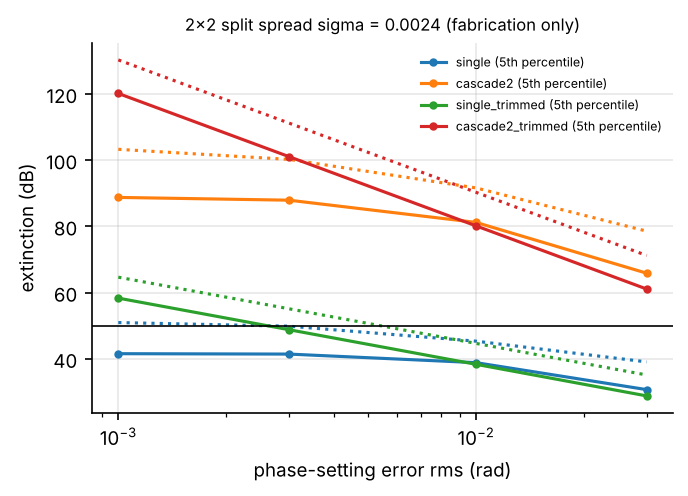
\includegraphics[width=0.7\linewidth]{m4_extinction.png}
\caption{Extinction of single, trimmed single, cascaded and trimmed cascaded MZI switches at 894.6~nm against the rms phase-setting error, from $2\times2$ transfer matrices with 4000 Monte Carlo trials per point. Solid lines with markers: 5th percentile; dotted lines: median. The $2\times2$ split ratio varies with the simulated fabrication spread $\sigma = 0.0024$ only (no design offset); arm amplitude imbalance 0.5\% rms. The horizontal line marks the 50~dB target.}
\label{fig:platform-extinction}
\end{figure}

A cascaded pair, as in~\cite{ZHAO}, reaches $\ge 50$~dB in every trial, with a 5th percentile of 88~dB. The 0.010 design offset of the first-pass $2\times2$ does not change this: it is shared by both couplers of an MZI, and two identical couplers still null exactly, so with the offset as a shifted mean the figures are unchanged ($P = 0.49$ for a single MZI, 88~dB for the cascade). An incoherent stray-light floor of $-70$~dB caps the cascade at 70~dB. For the AlN half-wave voltage at 894.6~nm, which we bracket between 84~V ($\lambda$-scaled from 74.7~V at 795~nm~\cite{ZHAO}) and 132~V (interpolated to 200~V at 1013~nm~\cite{ZHAO}), the 6.3~mrad limit of a single MZI requires driver noise below 0.17 to 0.27~V rms. The measured $V_\pi$ at 894.6~nm remains open ([VALUE?]).

Hence the binding constraints are polarisation and free-space crosstalk, not the interferometer. TM light is not nulled when the TE path is. For an input polarisation extinction of 20~dB, 50~dB at the output needs 24 to 30~dB of TM suppression after the chip; for 25~dB input, 19 to 25~dB. On 400~nm film bends cannot provide this (Sec.~\ref{sec:platform-wg}), hence a polariser in the free-space delivery path or a dedicated on-chip TE-pass element is required.

The settling of the switch is set by mechanical ringing of the AlN actuator, not by its 26~ns optical rise~\cite{ZHAO}. For an assumed single mode at $f_0 = 20$~MHz and $Q = 10$ ([VALUE?] for the real values), an unshaped step needs 0.98~\textmu s to reach $-50$~dB after switch-off. A two-impulse (ZV) shaper gives 24~ns, but 0.43~\textmu s with a 2\% error in $f_0$; a three-impulse (ZVD) shaper gives 49~ns with a 2\% error and 0.19~\textmu s with 5\%, at a 28~ns optical rise. Thus settling within 100~ns needs ZVD shaping with $f_0$ known to about 2\%.

The 16-output router (four stages of thermo-optically tuned MZI splitters) leaks at most $1.4\times10^{-3}$ into the worst unaddressed output (95th percentile) for a 30~mrad trim error, so with the cascaded output switch the idle-site extinction exceeds 110~dB (116~dB at 30~mrad). Its insertion loss is 5.0~dB, of which 3~dB is the assumed free-space delivery, so 16 sites at 20~\textmu W need about 1~mW at the input.

Two families of phase shifter serve different time scales. Thermo-optic shifters with a 2~\textmu m wide heater 2~\textmu m above the core need 84~mW for $\pi$ at 1064.4~nm (68~mW at 894.6~nm), with a 34~\textmu s rise and 16\% thermal crosstalk to a guide 10~\textmu m away. Isolation trenches reduce these to 54~mW and 2\%, and an additional undercut to 3~mW, at a 1.5~ms rise. The thermal conductivities and heat capacities in this model are recalled values, to be verified. Thermo-optic shifters suit slow router trims but not OPA updates at $\ge 100$~kHz. For the OPA, the PZT shifters of~\cite{MONT} ($V_\pi$ of 2.8~V at 532~nm, about 5.6~V at 1064.4~nm by wavelength scaling, 0.4~MHz bandwidth) settle in about 2~\textmu s, within a 5~\textmu s update period; their hysteresis is not known ([VALUE?]).

\subsection{System-level behaviour of the OPA}\label{sec:platform-opa}

\paragraph{Range and resolution.} The atom-plane field is a scaled copy of the slit-filtered OPA far field. The number of resolvable positions along the steering axis equals the channel number $N$, so the range at the atoms is $N\lambda/(4\,\mathrm{NA}\,F)$. Here, NA is the objective numerical aperture and $F$ the pupil fill. Table~\ref{tab:platform-field} gives the consequences at NA 0.5 and 1064.4~nm. At full fill, 64 channels steer over $\pm33$~\textmu m (17 sites at 4~\textmu m pitch), not $\pm100$~\textmu m, and cannot place more than about 15 tweezers on one row. More than 20 simultaneous tweezers on one row need 128 channels; at 0.75 fill they cover $\pm89$~\textmu m at 1.33 times the power per tweezer. Uniform channel amplitudes give 4.7\% first sidelobes along the steering axis; a Gaussian channel apodisation ($1/e^2$ at the aperture edge) lowers them to 0.9\% at a FWHM of 1.09~\textmu m. Section~\ref{sec:engine} builds on this count.

\begin{table}[htbp]\centering\small
\caption{Simulated steering field of the OPA (1D scalar Fourier optics, NA 0.5, 1064.4~nm). Here, the half-range is the usable one, in which the steered peak keeps at least half its on-axis value; ``sites'' is the number of 4~\textmu m sites on one row within it; and ``power'' is the relative power for equal depth.}
\label{tab:platform-field}
\begin{tabular}{cccccc}
\toprule
$N$ & fill $F$ & half-range (\textmu m) & sites & FWHM along $x$ (\textmu m) & power \\
\midrule
32 & 1.0 & 16 & 9 & 0.95 & 1.00 \\
64 & 1.0 & 33 & 17 & 0.95 & 1.00 \\
64 & 0.5 & 68 & 35 & 1.89 & 1.99 \\
128 & 1.0 & 67 & 33 & 0.94 & 1.00 \\
128 & 0.75 & 89 & 45 & 1.26 & 1.33 \\
256 & 1.0 & 134 & 67 & 0.94 & 1.00 \\
\bottomrule
\end{tabular}
\end{table}

\paragraph{Emitter type and pitch.} A Fourier-plane slit passes only the central diffraction zone, so the efficiency into it falls with emitter pitch: 0.65 at 1.5~\textmu m, 0.52 at 2~\textmu m and 0.34 at 3~\textmu m for the 0.6~\textmu m emitter guide (a wider emitter mode at the facet raises these, Sec.~\ref{sec:engine}). The minimum pitch is set by coupling between neighbouring emitters over their parallel length, for less than $-20$~dB power transfer: 1.46~\textmu m for an end-fire facet with an assumed 50~\textmu m parallel section, against 1.30, 1.56 and 1.82~\textmu m for gratings with 200, 100 and 50~nm etch (parallel lengths 20, 90 and 384~\textmu m). The gratings radiate 0.76, 0.72 and 0.68 upward at 8.9 to $10.0^\circ$, but their directionality oscillates with oxide thickness through the substrate reflection (0.42 to 0.76 over 2 to 4~\textmu m), the emission angle moves by $-0.10^\circ$/nm, and the 200~nm etch reflects 6\% back into the guide. Our choice of end-fire emitters is a compromise between two considerations. First, end-fire allows a dense pitch with short parallel sections, has no directionality loss and points independently of wavelength. However, it emits in plane and needs a relay to turn the beam towards the objective. The grating array becomes attractive only if a bottom reflector or two-layer grating is available.

\paragraph{Simultaneous tweezers by phase synthesis.} With weighted Gerchberg-Saxton alone ([REF?], recalled reference to be verified), light at untargeted lattice sites reaches 11 to 21\% of the tweezer intensity. A refinement that also penalises stray light and off-centre spots holds it at 3 to 7\%: for $N = 64$ with 8 or 12 tweezers the maximum stray is 0.056 and 0.053 and the maximum peak non-uniformity $(I_\mathrm{max}-I_\mathrm{min})/(I_\mathrm{max}+I_\mathrm{min})$ is 0.062 and 0.061; for $N = 128$ with 16 or 21 tweezers the stray is 0.054 and 0.057 and the non-uniformity 0.106. About 0.45 of the emitted power reaches the tweezers in all cases (four random target sets per case, one row along the steering axis). A 5.7\% stray at a static site corresponds to about 70~\textmu K under a 1.2~mK transport tweezer. This stray floor is one reason the steering engine of Section~\ref{sec:engine} avoids shared-aperture synthesis.

\paragraph{Phase accuracy.} For independent channel phase errors of rms $\sigma$, the position jitter at the atoms is $\sigma\sqrt{12/N}\,\lambda/(4\pi\,\mathrm{NA})$, which Monte Carlo reproduces to 2\%. Hence a 10~nm position error needs $\sigma \le 0.14$~rad at $N = 64$ (0.10~rad at 32, 0.19~rad at 128). Thus 8-bit phase resolution (7~mrad) is sufficient, and a PZT hysteresis error must stay below about 4\% of the applied phase at $N = 64$.

\paragraph{Update rate.} A tweezer moved by a staircase of OPA updates is excited because the staircase aliases the move spectrum to $|f_\mathrm{update}-f_\mathrm{trap}|$, where it can overlap the trap frequency. At the 1.2~mK transport depth the radial trap frequency is 84~kHz for $w_0 = 1.04$~\textmu m. As can be seen from Fig.~\ref{fig:platform-update}, a 100~kHz update then adds about 40 motional quanta to a 100~\textmu s, 4~\textmu m move and about 2,900 quanta to a 50~\textmu s move, against 0.005 and 0.2 for a smooth trajectory. At 200~kHz and above the staircase adds nothing measurable. Hence the $\ge 100$~kHz target of the proposal holds for 0.3~mK tweezers (42~kHz) but should read $\ge 200$~kHz for moves at 1.2~mK. Alternatively, lowering the depth to $\le 0.4$~mK during moves (48~kHz) with move times of $\ge 100$~\textmu s keeps 100~kHz: a 4~\textmu m move then adds 0.025 quanta (0.008 for a smooth trajectory).

\begin{figure}[htbp]\centering
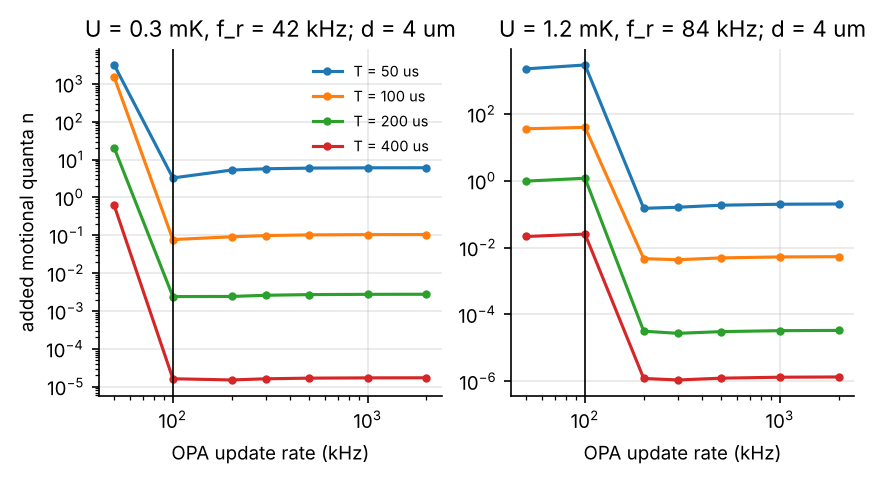
\includegraphics[width=0.85\linewidth]{m3_update_rate.png}
\caption{Motional quanta added to an atom by a 4~\textmu m OPA move against the update rate, for move durations $T$ of 50 to 400~\textmu s, at 0.3~mK ($f_r = 42$~kHz, left) and 1.2~mK ($f_r = 84$~kHz, right). Exact harmonic-oscillator result on the radial axis, atom initially in the ground state, minimum-jerk trajectory sampled and held at the update rate, $w_0 = 1.04$~\textmu m, polarisability 1160~a.u. The vertical line marks the 100~kHz target of the proposal. The curves are nearly flat from 200~kHz at 1.2~mK and from 100~kHz at 0.3~mK.}
\label{fig:platform-update}
\end{figure}

\paragraph{Loss budget.} For an end-fire OPA with $N = 128$, 21 tweezers and 2~\textmu m pitch, the chain from fibre to atoms is: edge coupler $-0.37$~dB, MMI tree $-0.27$~dB, propagation over 1~cm at 0.3~dB/cm (assumed) $-0.30$~dB, emitters with slit, pupil and synthesis $-3.43$~dB, and meta-objective transmission 0.7 (assumed) $-1.55$~dB, in total $-5.9$~dB. The grating case adds $-1.2$~dB of directionality ($-7.1$~dB for the best grating emitters). At 1.5~\textmu m pitch the slit term improves by about 1~dB. Against the ${\sim}10$~dB assumed in the proposal, the per-tweezer on-chip power falls from 66~mW to about 26~mW. This estimate excludes sidewall scattering.

\subsection{Phase-A error budget}\label{sec:platform-budget}

\paragraph{Idle-qubit error and trap depth.} The proposal's idle-qubit error for a switch of extinction ER is $(\pi^2/4)\,10^{-\mathrm{ER}/10}$, which gives $2.5\times10^{-5}$ at 50~dB when one Raman beam is addressed; we reproduce it. The proposal's trap depth is not reproduced: 6.6~mW in a Gaussian of $w_0 = 1.04$~\textmu m with a polarisability of 1160~a.u.\ gives 1.01~mK, not 1.2~mK; 1.2~mK needs 7.8~mW, or $w_0 = 0.96$~\textmu m. The OPA spot along the steering axis is 22\% brighter per watt than that Gaussian, which brings 6.6~mW to about 1.24~mK.

\paragraph{Addressing crosstalk.} Neighbour crosstalk of the 894.6~nm beams is set by the objective point-spread function, not by the chip. With a uniformly filled NA 0.5 pupil, the spot puts $1.0\times10^{-3}$ of its peak intensity on the 4~\textmu m neighbour, which gives a neighbour error of $2.5\times10^{-3}$, above the $10^{-3}$ budget. As can be seen from Fig.~\ref{fig:platform-crosstalk}, a Gaussian pupil fill truncated at 0.7 of the pupil radius brings this to $1.2\times10^{-4}$ (error $2.9\times10^{-4}$) at a spot FWHM of 1.13~\textmu m instead of 0.92~\textmu m. The model is aberration-free; a meta-objective with a Strehl ratio of 0.8 adds a halo that these figures do not include.

\begin{figure}[htbp]\centering
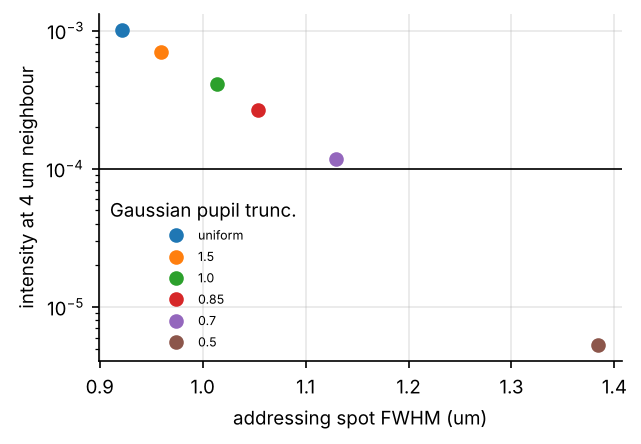
\includegraphics[width=0.6\linewidth]{m7_budget.png}
\caption{Intensity at the 4~\textmu m neighbour against the FWHM of the 894.6~nm addressing spot, for a uniform pupil and for Gaussian pupil fills truncated at 1.5, 1.0, 0.85, 0.7 and 0.5 of the pupil radius. Scalar Debye point-spread function, NA 0.5, aberration-free. The horizontal line marks $10^{-4}$.}
\label{fig:platform-crosstalk}
\end{figure}

\paragraph{Position and intensity noise.} The budget statement ``position noise $\le 10$~nm rms keeps transport survival $\ge 99\%$'' does not fix the heating rate, because heating depends on the noise spectral density at the trap frequency~\cite{OHARA}: $\dot{Q} = 4\pi^4 M\nu^4 S_x(\nu)$. Here, $M$ is the Cs mass (recalled, to be verified), $\nu$ the trap frequency and $S_x$ the position-noise spectral density. If 10~nm rms is white over 1~MHz, a 1.2~mK tweezer heats at about 7,700 quanta/s, about 0.8 quanta per 100~\textmu s move against a depth of about 300 quanta. Heating below 10 quanta/s needs $S_x(84~\mathrm{kHz}) \le 1.3\times10^{-25}$~m$^2$/Hz. In the same way, from $\Gamma = \pi^2\nu^2 S_I(2\nu)$~\cite{OHARA}, the relative intensity noise must satisfy $S_I(2\nu) \le 1.4\times10^{-11}$~/Hz at 1.2~mK for a parametric heating time of 1~s.

\paragraph{Power handling.} At 1.4~W into the input guide, with 0.3~dB/cm fully absorbed, the guide warms by 3.8~K and accrues 5.3~rad/cm of common-mode phase before the split. After the 64-way split each channel accrues at most 0.08~rad/cm, which the per-channel calibration absorbs.

\paragraph{Consequences for the specification.} The simulations imply six changes to the proposal's targets: (i) an OPA update rate of $\ge 200$~kHz for transport at 1.2~mK, or $\le 0.4$~mK during moves of $\ge 100$~\textmu s; (ii) a tweezer count tied to the channel count, with the steering field ($\pm33$~\textmu m at $N = 64$, $\pm68$~\textmu m at $N = 128$, $F = 1$) stated separately from the $\pm100$~\textmu m meta-objective field; (iii) about 6~dB (end-fire) to 7~dB (grating) of modelled chip and OPA loss, with 10~dB kept as the conservative value; (iv) position noise specified as $S_x(\nu_\mathrm{trap}) \le 1.3\times10^{-25}$~m$^2$/Hz, together with the 894.6~nm pupil apodisation needed for neighbour crosstalk $\le 10^{-4}$; (v) 7.8~mW, or the OPA spot, for 1.2~mK; and (vi) cascaded MZIs (or trimmed single MZIs with $\le 3$~mrad phase accuracy), an output polariser of $\ge 30$~dB on the 894.6~nm path, and ZVD-shaped drive for $\le 100$~ns settling. Item (ii) is superseded in its architectural part by the steering engine of Section~\ref{sec:engine}.

\section{The steering engine}\label{sec:engine}

This chapter derives the on-chip engine that moves twenty or more tweezers independently along one row, compares it with the switched-port star coupler, and gives the beam-propagation design D1 with its simulated errors, power cost and limits.

\subsection{The requirement and what an AOD supplies}\label{sec:engine-req}

Section~\ref{sec:platform-opa} showed that the number of resolvable positions of an OPA along its steering axis equals its channel number $N$: 64 channels place at most about 15 tweezers on a row of 4~\textmu m sites, and more than 20 need 128 channels. Count alone is not the requirement, however. Rearrangement needs each tweezer to move on its own, as the tones of an acousto-optic deflector (AOD) do. An AOD owes this to two physical ingredients (standard AOD physics, [REF?] for a citable source): (i) frequency tagging, since each RF tone shifts its diffracted light by its own frequency, so that tweezers from different tones add incoherently on average and each tone's amplitude sets one tweezer's depth; and (ii) a time-delay medium, since the acoustic transit time across the aperture converts each tone's frequency into its own angle, and the number of resolvable spots is the RF bandwidth times the transit time. The independence is per axis. A single AOD moves its spots independently along one line, and crossed AODs give a grid of row and column tones rather than independent 2D positions (ref.~[17] of the proposal~\cite{proposal}). Hence the fair target for an integrated engine is a 1D AOD along a row.

A shared-arm OPA, in which every tweezer uses every arm, has neither ingredient, and phase-only synthesis couples all tweezers. We tested this directly on a 128-channel OPA with 20 synthesised tweezers. Removing one of them by warm-started re-synthesis (that site added to the dark points) leaves 1.9 to 3.3\% of the tweezer intensity at its site ($-15$ to $-17$~dB), changes the 19 kept tweezers by up to 12\%, and along a linear phase path between the two patterns the kept tweezers deviate by up to 19\%. Stray light at untargeted sites stays at about 2\%. Such an engine cannot gate 894.6~nm light at 50~dB, and it perturbs every other atom whenever one tweezer is switched.

Table~\ref{tab:engine-routes} lists the routes we considered for supplying an equivalent of at least one AOD ingredient. Route~E, the sliding-window focal-plane OPA, is the only one that works at a single optical frequency, uses only components already in the proposal (SiN star coupler, MZI trees, PZT or AlN shifters) and needs no new physics. Complex synthesis on the arms (A$'$) is a fallback with fewer optical elements, but needs amplitude modulation on every arm and power headroom, because moving one tweezer changes the optimum. The wavelength-addressed route (D) is excluded by the chromatic focal shift of a diffractive meta-objective unless that objective is made achromatic over several nanometres around 1064~nm.

\begin{table}[htbp]\centering\small
\caption{Routes to independently steered tweezers on one row (20 tweezers). Efficiencies are simulated (E, A$'$, F) or derived (D, G, T). The surface-acoustic-wave velocity used for route G ($\sim$5~km/s) is recalled, to be verified for an AlN/SiN/SiO$_2$ stack.}
\label{tab:engine-routes}
\begin{tabularx}{\linewidth}{@{}p{0.2\linewidth}Xp{0.13\linewidth}X@{}}
\toprule
Route & Source of independence & Efficiency & Show-stopper or cost \\
\midrule
E: sliding-window focal-plane OPA & tweezers on separate ports (position basis), linear superposition & 0.40 at centre, 0.19 at field edge & 127 fast splitters and 128 phase shifters; ${\sim}1\%$ per-port accuracy \\
A$'$: complex synthesis on the arms & linear superposition of 20 phase ramps (amplitude and phase per arm) & 0.75 (peak-to-mean 1.34) & 128 amplitude and phase modulators; power headroom \\
F: AOD emulation on the arms & one RF tone per tweezer: frequency tags and per-tone phase ramps & 0.44 (peak-to-mean 2.28) & 256 RF-driven modulators; intermodulation ghosts from modulator nonlinearity \\
D: wavelength-addressed dispersive OPA & optical frequency tags and delay lines & high (passive) & focal shift 14~\textmu m/nm allows only $\pm71$~pm ($\pm19$~GHz); 5~GHz per site needs 6.7~m of delay lines \\
G: integrated surface-acoustic-wave deflector & a literal AOD in the slab & unknown & 128 spots need 640~MHz of RF bandwidth on 1~mm, 128~MHz on 5~mm; photoelastic response of SiN not established \\
T: time-multiplexed OPA & time-averaged potentials & 1 per slot & 17~MHz pattern rate, 60~ns slots, 20 times the peak intensity \\
\bottomrule
\end{tabularx}
\end{table}

\subsection{The switched-port star coupler and its limits}\label{sec:engine-star}

Before route~E we designed an engine that keeps per-tweezer switching but gives up independent motion. Each tweezer has its own input port and MZI switch; the ports illuminate a common 128-arm phased array through a free-propagation region (FPR) of radius $R$; and a phase ramp on the arms moves all lit tweezers together. One chip per wavelength carries (i) edge-coupled input, (ii) a $1\times32$ tunable-splitter tree that sends power only to lit ports, so that the power per tweezer does not depend on how many are lit, (iii) 20 port switches (thermo-optic at 1064.4~nm, two cascaded AlN MZIs at 894.6~nm), (iv) the FPR, (v) 128 arms, 1.7~\textmu m wide at the FPR edge (0.3~\textmu m gaps), each with a phase shifter, and (vi) 128 end-fire emitters at 1.5~\textmu m pitch, followed by the slit-filtered relay and NA 0.5 meta-objective; a dichroic combines the two chips. Port $j$ imposes a linear phase $k_s d_j p_a/R$ per arm, which steers its beam to $\sin\theta_j = n_s d_j p_a/(R\,p_\mathrm{out})$. Here, $k_s$ and $n_s$ are the slab wavenumber and index, $d_j$ is the port offset, $p_a$ the arm pitch at the FPR and $p_\mathrm{out}$ the emitter pitch. The relay maps $x = \sin\theta\,N p_\mathrm{out}/(2\,\mathrm{NA})$, so a 4~\textmu m step is $\sin\theta = 0.0208$ for $N = 128$ and $p_\mathrm{out} = 1.5$~\textmu m.

Each port illuminates all arms with the far field of its taper mode, which apodises the array. The tails of this envelope set the light a lit tweezer leaves on its neighbours and the interference between lit ports, whose relative phases drift with the router temperature. Table~\ref{tab:engine-apod} shows the trade-off: a standard star coupler ($1/e^2$ at the outer arms) leaves $1.2\times10^{-3}$ on the neighbour and 19\% peak spread, an order of magnitude above the $10^{-4}$ target. A narrower envelope needs a smaller FPR radius, which brings the ports closer together; widening the input taper restores the radius, and its mode, closer to Gaussian, lowers the tails further. The final designs use 1.4~\textmu m tapers at 1.89~\textmu m pitch with $R = 223$~\textmu m at 1064.4~nm, and 1.0~\textmu m tapers at 1.64~\textmu m pitch with $R = 197$~\textmu m at 894.6~nm, both at a nominal $e^{-6}$ envelope (realised $2.7\times10^{-5}$ and $7.2\times10^{-6}$, because the wide-taper modes are not Gaussian). Two 1.4~\textmu m tapers 0.49~\textmu m apart have a coupling length of 1.33~mm, so their ${\sim}20$~\textmu m convergence transfers well below $-20$~dB. We keep this cleaner design at 1064.4~nm although an $e^{-5}$ envelope gives 9\% more depth per watt, because its 3\% peak spread and $4\times10^{-5}$ neighbour light would make tweezer depths depend on drifting port phases. With $N = 96$ the half-range would be 51~\textmu m (1064.4~nm) or 43~\textmu m (894.6~nm), leaving only 5 to 13~\textmu m of collective travel for a 20-site row ($\pm38$~\textmu m); $N = 128$ gives $\pm68$ and $\pm57$~\textmu m. Table~\ref{tab:engine-star} summarises the final designs.

\begin{table}[htbp]\centering\small
\caption{Effect of the arm-power envelope of the star coupler at 1064.4~nm (simulated, 2D paraxial FPR, 0.6~\textmu m input taper). ``Spread'' is the largest variation of peak intensity with all 20 ports lit at random relative phases.}
\label{tab:engine-apod}
\begin{tabular}{cccc}
\toprule
outer-arm envelope (nominal) & FWHM (\textmu m) & neighbour / peak & spread, 20 lit \\
\midrule
$e^{-2}$ & 1.10 & $1.2\times10^{-3}$ & 19\% \\
$e^{-4}$ & 1.24 & $4.2\times10^{-4}$ & 11\% \\
$e^{-6}$ & 1.38 & $9.6\times10^{-5}$ & 5.8\% \\
$e^{-8}$ & 1.52 & $1.3\times10^{-5}$ & 2.0\% \\
\bottomrule
\end{tabular}
\end{table}

\begin{table}[htbp]\centering\small
\caption{Simulated performance of the switched-port star-coupler OPA (128 emitters, 20 ports on a row of 4~\textmu m sites). Fibre power assumes a 1.04~\textmu m Gaussian profile along the cross axis, 0.3~dB/cm propagation and meta-objective transmission 0.7 (both assumed).}
\label{tab:engine-star}
\begin{tabular}{@{}p{0.31\linewidth}p{0.29\linewidth}p{0.29\linewidth}@{}}
\toprule
& 1064.4 nm (transport) & 894.6 nm (addressing) \\
\midrule
spot FWHM along the row & 1.52~\textmu m & 1.27~\textmu m \\
intensity at the 4~\textmu m neighbour / peak & $1.0\times10^{-6}$ & $3.5\times10^{-6}$ (error $8.5\times10^{-6}$) \\
peak spread, all 20 lit, random port phases & $\le 0.73\%$ & $\le 0.89\%$ \\
stray at unlit sites (10 of 20 lit) & $\le 1.2\times10^{-5}$ & $\le 2.1\times10^{-5}$ \\
static position error of a spot & $\le 6$~nm & $\le 5$~nm \\
switch per port & one trimmed thermo-optic MZI & two cascaded AlN MZIs \\
extinction needed & $\ge 31$~dB (1~\textmu K residual at 1.2~mK) & $\ge 50$~dB (idle error $2.5\times10^{-5}$) \\
fibre power & 33 to 43~mW per tweezer; 0.74~W for 20 & $\le 0.14$~mW per site; 2.4~mW for 20 \\
\bottomrule
\end{tabular}
\end{table}

The collective move is one linear ramp: a single analog waveform drives the 128 arm shifters with fixed gains $n = 0\dots127$, plus slow per-arm calibration offsets, and a continuous ramp has no staircase, which removes the update-rate heating of Sec.~\ref{sec:platform-opa}. With all 20 lit, collective shifts of 4 and 24~\textmu m change the peaks by $-2.5/{+2.3}\%$ and $-16.7/{+10.3}\%$, following the emitter element factor; this is pre-compensated through the port powers. The element-factor slope also gives the outer spots a static offset of up to 25~nm at 1064.4~nm (26~nm at a 24~\textmu m shift; 5 to 6~nm at 894.6~nm), which changes by less than 2~nm over a 24~\textmu m sweep and is calibrated out. At 894.6~nm the switch leak equals the $3.5\times10^{-6}$ optical tail of a lit neighbour at 54.6~dB, well inside the 66 to 88~dB of the cascaded pair; at 1064.4~nm a trimmed thermo-optic MZI exceeds the 31~dB needed (5th percentile 38~dB at 10~mrad, computed at 894.6~nm and to be repeated at 1064.4~nm).

The limits of this engine are structural. All lit tweezers move by the same displacement, so a sorting sequence must be built from parallel moves, as with AODs, although at one optical frequency, so that two tweezers brought together do not beat. The two chips need about 380 electrical channels, against the 32 to 64-channel OPA and 16-channel router of the proposal, and the 51 heaters of the 1064.4~nm chip draw about 2.1~W without trenches (about 0.1~W with trenches and undercut). The FPR model is 2D and paraxial. We retain this design for the 894.6~nm addressing beams (Sec.~\ref{sec:engine-E}), where its per-port cascaded switch sets the off-state.

\subsection{Sliding-window focal-plane OPA (route E)}\label{sec:engine-E}

Route~E replaces the few switched ports by a dense row of 128 input ports, one per resolvable spot. The FPR radius is $R = N p_a p_\mathrm{port}/\lambda_s$, which makes port $k$ form a spot at $x_k = k\lambda/(2\,\mathrm{NA})$, i.e.\ 1.064~\textmu m per port at the atoms. Here, $p_\mathrm{port}$ is the port pitch and $\lambda_s$ the wavelength in the slab. A tweezer is a Gaussian-weighted group of about five ports and moves by sliding this window. In this position basis different tweezers use different ports, so their fields add linearly and interfere only through their tails. In addition, two tweezers can approach without interference if their relative phase is set to $\pi/2$, since the cross term of two real fields then vanishes; this is a control an AOD lacks, where approaching tones beat at their frequency difference. The first, paraxial geometry had 128 ports 1.7~\textmu m wide at 2.0~\textmu m pitch, $R = 886$~\textmu m, 128 arms (1.7~\textmu m wide at 2.0~\textmu m pitch) and 128 end-fire emitters at 1.5~\textmu m pitch. Adjacent ports at 0.3~\textmu m gaps have a coupling length of 625~\textmu m, so the ${\sim}20$~\textmu m over which they converge transfers below $-20$~dB.

The window width $\sigma$ (in ports) sets the spot apodisation. Our choice of $\sigma = 0.9$ is a compromise between two considerations. First, a narrow window gives a small spot and hence more depth per watt. However, it leaves a larger position nonlinearity and peak ripple as the window slides between ports (Fig.~\ref{fig:engine-window}): 18~nm and 3.4\% at $\sigma = 0.8$, 8.6~nm and 1.5\% at 0.9, 3.7~nm and 0.55\% at 1.0, and 0.5~nm and 0.07\% at 1.2, at spot FWHMs of 1.51, 1.66, 1.82 and 2.16~\textmu m and neighbour intensities at 4~\textmu m of $1.1\times10^{-4}$, $2.0\times10^{-5}$, $2\times10^{-6}$ and $7.6\times10^{-5}$. Both residuals are deterministic in the window position and are removed by a lookup table, together with the fall-off of delivered power from 0.40 at the centre to 0.19 at $\pm64$~\textmu m.

\begin{figure}[htbp]\centering
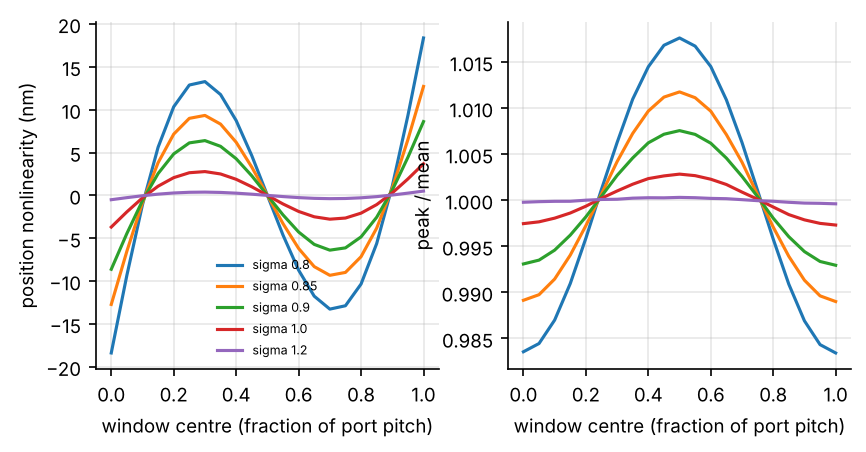
\includegraphics[width=0.75\linewidth]{m9_E_window.png}
\caption{Uncalibrated response of a sliding Gaussian window in the first (paraxial) route-E design, as the window centre moves across one port pitch, for window widths $\sigma = 0.8$ to 1.2 ports. Left: deviation of the spot position from a linear map. Right: peak intensity relative to its mean. 2D paraxial FPR with isolated port and arm modes, $N = 128$ ports at 2.0~\textmu m pitch (1.7~\textmu m wide), $R = 886$~\textmu m, 128 arms, emitter pitch 1.5~\textmu m, NA 0.5, 1064.4~nm. Both curves are periodic in the port pitch and are removed by a lookup table.}
\label{fig:engine-window}
\end{figure}

With 20 tweezers at random positions over $\pm60$~\textmu m and $\sigma = 0.9$ (calibrated), a tweezer moved by 0.1 to 4~\textmu m lands within 0.9~nm of its target with a peak change of at most 0.10\%, while the other 19 shift by at most 1.5~nm and 0.19\%. Removing a window leaves $8.9\times10^{-6}$ of the tweezer intensity at its site and changes the others by at most 0.08\%. The static peak spread of the 20 is 1.4\% with depth equalised by the tree. Two tweezers in quadrature at 2.5~\textmu m pull each other by 3.5~nm with a 0.16\% peak change, against 146~nm and 9.5\% in phase.

The cost lies in the actuators and their accuracy: 127 fast tunable splitters and 128 port phase shifters per chip. Because each tweezer is set by only about five ports, per-port errors average little. Per-port amplitude and phase errors of 0.3\%/3~mrad, 1\%/10~mrad and 3\%/30~mrad rms give position noise of 3.1, 9.4 and 28~nm and peak noise of 0.5, 1.9 and 5.6\%. Thus 10~nm needs about 1\% and 10~mrad, about 15 times tighter than the arm-side OPA (0.14~rad at $N = 64$, Sec.~\ref{sec:platform-opa}), and PZT hysteresis ([VALUE?]) must be corrected, for example by closed-loop calibration against on-chip taps. A moving tweezer is updated through the tree, so the staircase result applies: $\ge 200$~kHz updates at 1.2~mK, which PZT shifters (0.4~MHz~\cite{MONT}) meet and thermo-optic shifters (34~\textmu s rise) do not. The node settings follow in closed form from the desired port amplitudes, since each node splits in the ratio of the powers of its two subtrees, so an FPGA can compute them in real time. A tweezer is switched by ramping its window through the tree adiabatically ($\ge 100$~\textmu s), and its off-state is then set by the extinction of the tree nodes.

This last point decides the 894.6~nm engine. Raman gates act on atoms in static traps, and the addressed Raman leg must keep a fixed frequency relative to the global leg, so frequency tagging is unavailable at 894.6~nm. Route~E there would give steerable addressing with an off-state set by the tree nodes, rather than by a cascaded switch per beam. The switched-port star coupler of Sec.~\ref{sec:engine-star} therefore remains the addressing engine, and route~E the transport engine at 1064.4~nm.

\subsection{Design D1 by beam propagation}\label{sec:engine-D1}

The paraxial model above treats ports and arms as isolated and the FPR as aberration-free. Dense ports at 0.3~\textmu m gaps couple, and an AWG-type star coupler needs a full propagation design. Since the 400~nm film is uniform and fully etched, every guide and the slab share one vertical mode, and a lateral effective-index model carries the star-coupler physics. The plain effective-index model overestimates lateral confinement: its coupling lengths are 31 to 36\% short of the 3D vector-FEM values. We therefore calibrate the lateral core and cladding indices (1.8423 and 1.3551) to the vector-FEM effective indices of 0.6, 1.0 and 1.7~\textmu m guides (residuals $\le 4.3\times10^{-4}$) and to the coupling length of the dense ports (622 against 625~\textmu m); a held-out check on 1.4~\textmu m guides at 0.49~\textmu m gap agrees to 3\%, and narrow, widely spaced guides (off by 29\%) couple negligibly in the design. Propagation uses a 2D wide-angle (Pad\'e (1,1)) Crank-Nicolson beam-propagation method (BPM) with the TM-type lateral operator that matches the chip TE mode, all ports propagated together ($\Delta x = 0.04$~\textmu m, $\Delta z = 0.125$~\textmu m; capture converged to 0.5\%). On a reduced 8-port, 8-arm coupler, 2D FDTD and BPM agree in arm field with fidelity 0.997 (centre port) to 0.93 (edge port, rising to 0.981 at finer FDTD resolution) and in capture to 2 to 5\%, the residual being dominated by FDTD discretisation. For fast optimisation an exact-path Rayleigh-Sommerfeld model reproduces the full $128\times128$ BPM to within 1\% in capture and with arm-field fidelity 0.996 to 0.9996 (0.96 at the two extreme ports, where taper coupling matters); on the optimised design both give the same field-averaged efficiency to 0.6\%.

The propagation revealed two effects absent from the paraxial model. (i) The confocal coupler (ports on an arc of radius $R$) is aberrated: each off-axis port's arm phases deviate from a straight line by up to 1.3~rad peak-to-peak at the edge port (0.43~rad half-way out). Arm trims cannot remove this because it depends on the port. Placing the ports on an arc of radius $0.555R$, close to the Rowland circle, halves it over the field of use, and with 192 arms the worst residual is 0.08~rad rms; the different piston phase this gives each port is removed by static port trims. (ii) Neighbouring ports exchange light in the converging tapers. With fixed Gaussian windows this broadens the spot tails, and moving one of 20 tweezers then changes the others by up to 7~nm and 1.1\%. Both effects are linear and static, which the synthesis of Sec.~\ref{sec:engine-LS} exploits.

We then optimised the geometry for the field-averaged laser power per tweezer at equal depth, i.e.\ the harmonic mean of the peak intensity per unit port power over $|x| \le 60$~\textmu m, under the constraints of a neighbour intensity at 4~\textmu m of $\le 10^{-4}$, gaps $\ge 0.3$~\textmu m, and 128 ports (the fast actuators) fixed. The roll-off across the field has one origin on both sides of the chip, scan loss: the arms capture tilted light from off-axis ports, and the emitters radiate tilted beams, each with an element pattern that falls across its angular range. Two levers act on it (Fig.~\ref{fig:engine-opt}). Oversampling, i.e.\ more arms and emitters than ports, confines the ports to the central part of the arms' angular range and raises the edge capture from 0.44 to 0.54 with 192 arms. Arms and emitters carry only static trims in route~E, so this costs area and slow heaters, not fast actuators; 256 arms would add 7\% for 64 more trims and a 1.8~mm slab. Wider emitter facets narrow the element pattern and raise the relay transmission at the centre from 0.64 (0.6~\textmu m) to 0.84 (1.2~\textmu m at 1.5~\textmu m pitch). With 0.5~\textmu m gaps the transmission saturates near 0.74 to 0.76 for any pitch from 1.5 to 2.2~\textmu m, so the 0.3~\textmu m gap of the 1.2~\textmu m facet buys the last 10\%; its coupling length of 227~\textmu m limits the wide facet section to about 15~\textmu m. At the slab, the widest ports and arms (1.7~\textmu m at 2.0~\textmu m pitch) give a field-averaged efficiency of 0.261 against 0.18 to 0.24 for 1.2 to 1.5~\textmu m widths, because fill factor outweighs the slightly better angular acceptance of narrow arms. Narrowing the window from 0.9 to 0.85 ports gains 5\% but raises the neighbour intensity to $4.8\times10^{-5}$; we adopt least-squares synthesis with a 1.68~\textmu m target instead.

\begin{figure}[htbp]\centering
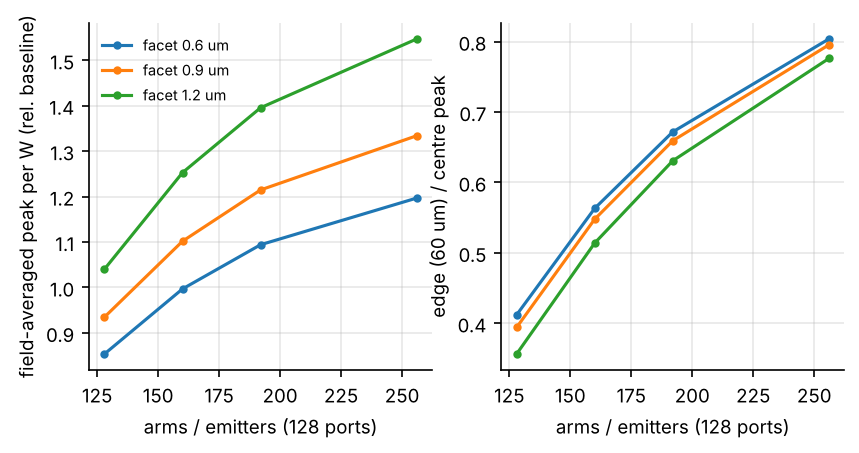
\includegraphics[width=0.75\linewidth]{m11_stage1.png}
\caption{Geometry optimisation of the route-E star coupler with 128 ports, against the number of arms and emitters, for emitter facets of 0.6, 0.9 and 1.2~\textmu m at 1.5~\textmu m pitch. Left: field-averaged peak intensity per unit port power (harmonic mean over $|x| \le 60$~\textmu m), relative to the confocal $128\times128$ design with 0.6~\textmu m facets. Right: peak at the field edge ($x = 60$~\textmu m) relative to the centre. Exact-path (Rayleigh-Sommerfeld) star-coupler model, ports on a Rowland-type arc of radius $0.555R$, ports and arms 1.7~\textmu m wide at 2.0~\textmu m pitch, Gaussian window $\sigma = 0.9$ ports, NA 0.5. D1 is the 192-arm, 1.2~\textmu m-facet point (gain 1.51, edge ratio 0.71).}
\label{fig:engine-opt}
\end{figure}

The resulting design D1 has 128 input ports and 192 arms, both 1.7~\textmu m wide at 2.0~\textmu m pitch at the slab (0.3~\textmu m gaps); a slab radius $R = 1329$~\textmu m; ports on an arc of radius $0.555R$ through the slab vertex, pointing at the arm-array centre; arms on an arc of radius $R$ with 30~\textmu m tapers to 0.6~\textmu m guides; 192 end-fire emitters at 1.5~\textmu m pitch with 1.2~\textmu m facets (facet taper $\le 15$~\textmu m); static phase trims on all arms and ports; and port amplitudes from least-squares synthesis.

\subsection{Least-squares port synthesis and residual errors}\label{sec:engine-LS}

Instead of fixed Gaussian windows, we compute the port amplitudes by least squares on the calibrated port-to-atom response, with the target spots as the objective. Because port coupling and aberration are linear and static, the synthesis removes them, at a cost of 1 to 2\% in efficiency, and it equalises depth over the field without a lookup table. Each update is one product with a precomputed $128\times n$ matrix. Table~\ref{tab:engine-D1} compares D1 with the first (confocal $128\times128$) design, both verified by BPM of the full structure with the calibrated effective-index model and least-squares synthesis.

\begin{table}[htbp]\centering\small
\caption{Simulated performance of the route-E engine: first confocal design against the optimised design D1 (full BPM, least-squares port synthesis, 20 tweezers over $\pm60$~\textmu m). Laser power uses facet $-0.37$~dB, 7-stage tunable tree $-0.39$~dB, 1~cm at 0.3~dB/cm and meta-objective transmission 0.7 (both assumed), and a 1.04~\textmu m Gaussian profile across the row; see the text for the revised value.}
\label{tab:engine-D1}
\begin{tabular}{@{}p{0.42\linewidth}cc@{}}
\toprule
quantity & first design & D1 \\
& ($128\times128$, confocal) & \\
\midrule
field-averaged peak per unit port power (relative) & 1.00 & 1.50 \\
edge (60~\textmu m) / centre peak & 0.52 & 0.70 \\
residual arm-phase aberration, worst port & $\le 1.3$~rad pk-pk & $\le 0.08$~rad rms \\
others' change when one of 20 moves by up to 4~\textmu m & $\le 3.5$~nm, $\le 0.12\%$ & $\le 3.5$~nm, $\le 0.11\%$ \\
residual at a switched-off site & $1.3\times10^{-6}$ & $1.6\times10^{-6}$ \\
static peak spread of 20 tweezers & 0.56\% & 0.52\% \\
spot FWHM along the row & 1.71~\textmu m & 1.71~\textmu m \\
laser power per 1.2~mK tweezer, field mean (fibre) & ${\sim}65$~mW & ${\sim}43$~mW \\
20 tweezers over $\pm60$~\textmu m & ${\sim}1.3$~W & ${\sim}0.86$~W \\
\bottomrule
\end{tabular}
\end{table}

Under full propagation with synthesis the others' displacement is up to 3.5~nm rather than the 1.5~nm of the paraxial windows (Sec.~\ref{sec:engine-E}), while the peak change, switch-off residual and peak spread are smaller. The per-port actuator accuracy, about 1\% and 10~mrad for 10~nm of position noise, is not relaxed by the synthesis and remains the main requirement on the hardware.

\subsection{Power per tweezer}\label{sec:engine-power}

The loss chain from fibre to atoms is the facet ($-0.37$~dB), the 7-stage tunable tree ($-0.39$~dB), 1~cm of propagation at 0.3~dB/cm (assumed, $-0.3$~dB), the simulated FPR, arms, emitters, slit and pupil, and a meta-objective transmission of 0.7 (assumed). In the first paraxial design a 1.2~mK tweezer needs 48~mW at the fibre at the field centre and 102~mW at the edge; equalising depth costs a mean factor of 1.34, so 20 tweezers spread over $\pm60$~\textmu m need about 1.3~W, and restricting operation to $\pm40$~\textmu m lowers the mean factor. D1 brings the field mean to about 43~mW (0.86~W for 20), a factor 1.5 in efficiency. However, both figures omit the cross axis and the emitter facet loss (about 21\% into air). With both included and a collimator glued to the facets, a 1.2~mK tweezer needs about 57~mW (\texttt{docs/stacked\_relay.md}, \texttt{docs/collimator.md}); this is the current value. For comparison, the switched-port star coupler, computed with the same Gaussian cross-axis profile, needs 33 to 43~mW per tweezer, and the proposal assumes 1.4~W for 21 tweezers.

\subsection{Limits}\label{sec:engine-limits}

The model is 2D with a calibrated effective index. The residual 3D effects, polarisation coupling at sidewalls and slab-edge scattering, are not computed, and the 3D excess loss of the dense-port FPR is open ([VALUE?]). Fabrication variation of the 0.3~\textmu m gaps and of the taper geometry has not been simulated; static errors are absorbed by the trims and the measured response matrix, but the arm phase errors after fabrication, which set the trim range, are not known ([VALUE?]). The relay and objective are scalar and aberration-free, so a meta-objective with a Strehl ratio of 0.8 adds a halo not included in the crosstalk figures. Steering is along one row; the second axis needs a second engine or an OPA-AOD hybrid. The hardware load of D1 is 255 fast actuators (127 tree splitters and 128 port phase shifters, which also carry the port trims) and 192 static arm trims, with PZT shifter footprint, hysteresis and long-term drift after closed-loop calibration still open ([VALUE?]). The procedure that measures the port-to-atom response on the device, on which the least-squares synthesis rests, has yet to be defined.

\section{Rows of engines: the stacked-chip relay}\label{sec:rows}

One focal-plane engine steers one row of tweezers along $x$. This section describes how 16 such chips are
stacked and imaged onto the atoms as 16 independent rows, what the collimator in front of each chip must do,
and how the rows are kept mutually incoherent without one frequency shifter per chip.

The result is as follows. Sixteen chips of design D1 (128 input ports, 192 arms and emitters,
Sec.~\ref{sec:engine}), stacked at 0.5~mm pitch, each with its own fast-axis collimator (FAC), are imaged as
16 rows 4~\textmu m apart through the NA~0.5 objective at 1064.4~nm. The adopted collimator is a glued
Weierstrass block followed by a two-asphere aplanat. With it, a 1.2~mK tweezer needs 57~mW of laser power.
A full row produces a crosstalk of $1.8\times10^{-4}$ at the neighbouring row (ideal collimator). Rows are as independent as
the tweezers within a row provided their relative optical phase is randomised much faster than the trap
period. One phase modulator on the common seed, driven with Gaussian noise, together with different fibre
delays per chip, does this. The costs are a collimator alignment of $\pm0.1$~\textmu m in height, a
diffraction-limited collimator at NA~0.9, and two rules on spectral filtering and parasitic reflections in
the laser chain. All values are simulated in scalar wave optics (with ray tracing and 2D FDTD where stated)
or derived from those simulations; the code and results are listed in \texttt{docs/stacked\_relay.md},
\texttt{docs/collimator.md}, \texttt{docs/row\_coherence.md} and \texttt{docs/pm\_am.md}.

\subsection{Anamorphic layout}\label{sec:rows-layout}

The relay treats the two axes differently. In $x$, the relay of Sec.~\ref{sec:engine} images the emitter plane
onto the objective pupil, so the atoms see the far field of the chip. In $y$, each chip's facet sits in the
front focal plane of its own cylindrical collimator. The back focal planes of the collimators form a plane
$S$, which a common $y$ lens group of effective focal length $F_y$ Fourier transforms onto the pupil. Thus $S$
is imaged onto the atoms with magnification $f_\mathrm{obj}/F_y = 1/D$, and chip $m$ lands at
$y_m = m\,d_c/D$. Here, $d_c$ is the chip pitch, $D$ the demagnification of the stack, and
$f_\mathrm{obj}=17.3$~mm the objective focal length (pupil radius $f_\mathrm{obj}\,\mathrm{NA}$ at a working
distance of 15~mm). At the same time, the pupil is an image of the facet in both axes, with magnification 60
in $x$ and 12,400 in $y$. Because each chip has its own collimator centred on its facet, all 16 facet images
overlap in the pupil, and the row offsets come only from the tilt $y_m/F_y$. A single common collimator would
not work: it would place the 16 facet images side by side in the pupil.

The free parameter of the $y$ design is the pupil radius referred back to the facet,
$\beta = \mathrm{NA}\,f_\mathrm{FAC}/D$. Here, $f_\mathrm{FAC}$ is the collimator focal length and NA~$=0.5$.
The parameter $\beta$ plays the role of the pupil fill (Sec.~\ref{sec:rows-fill}). The row pitch fixes $D$,
and $\beta$ then fixes $f_\mathrm{FAC}$. Table~\ref{tab:rows-layout} gives the first-order layout for
$\beta = 0.7$~\textmu m (thin cylindrical lenses; ABCD matrices of both axes checked).

\begin{table}[htbp]\centering\small
\caption{First-order layout of the anamorphic relay for 16 chips at 0.5~mm pitch, $\beta=0.7$~\textmu m,
FAC NA~0.9. Thin lenses; derived. The 4~\textmu m row pitch is the design point.}
\label{tab:rows-layout}
\begin{tabular}{cccccc}
\toprule
row pitch & $D$ & $F_y$ & $f_\mathrm{FAC}$ & collimated half-height & facet to pupil \\
\midrule
3~\textmu m & 167 & 2.89~m & 233~\textmu m & 210~\textmu m & 439~mm \\
4~\textmu m & 125 & 2.17~m & 175~\textmu m & 158~\textmu m & 382~mm \\
5~\textmu m & 100 & 1.73~m & 140~\textmu m & 126~\textmu m & 347~mm \\
6~\textmu m & 83 & 1.44~m & 117~\textmu m & 105~\textmu m & 324~mm \\
\bottomrule
\end{tabular}
\end{table}

At 4~\textmu m row pitch ($D=125$), the long effective focal length is realised as a $25\times$ demagnifying
$y$ telescope (focal lengths 100~mm and 4~mm) followed by an 86.6~mm Fourier lens. The $x$ relay is a 4f pair
(3.12~mm and 187.7~mm) with the Fourier slit 6.2~mm from the facets. Both pupils coincide 382~mm from the
facets. The Lagrange invariant matches on both sides: a stack half-height of 4~mm times a collimated NA of
0.0022 equals the atom half-field of 30~\textmu m times 0.5 times the fill. The collimated beams
(158~\textmu m half-height) fit within the 250~\textmu m half-pitch, as they do at 3~\textmu m row pitch
(210~\textmu m). This layout is first order; a real lens design of the anamorphic relay over its 8~mm field
has not been made.

\subsection{Facet mode, pupil fill and crosstalk floor}\label{sec:rows-fill}

\paragraph{Validity of the $y$ results.} All $y$-axis results of this section (pupil fill, collimator
performance, row crosstalk and alignment tolerances) were computed for light with no $x$ direction component,
$s_x=0$. However, a tweezer at position $x_a$ along the row is made of light with $s_x = x_a/288$~\textmu m
(for D1), and the cylindrical collimator then acts with effective indices $\sqrt{n^2-s_x^2}$. The adopted
collimator (Sec.~\ref{sec:rows-collimator}) therefore defocuses the facet by $-99\,s_x^2$~\textmu m. The $y$
figures below hold near the row centre only: the peak falls to 0.97 at $x_a=30$~\textmu m and to 0.48 at
60~\textmu m. With the best common focus offset, a row is usable over $|x_a|\le 45$~\textmu m, less than the
$\pm60$~\textmu m row of D1 used in the crosstalk tests below. Section~\ref{sec:combine} gives the details.

\paragraph{The facet.} The D1 emitter facet ($1.2\times0.4$~\textmu m SiN in oxide) has a vertical mode of
$1/e^2$ equivalent radius 0.39~\textmu m. It radiates into air with a far-field $1/e^2$ half-angle of
$\sin\theta=0.86$. A collimator of NA~0.8 captures 96\% of this light, one of NA~0.9 captures 98.8\%.
Thinning the SiN at the facet expands the vertical mode, but it also expands the lateral one. At 100~nm the
far-field NA drops to 0.51, but the coupling length of adjacent emitters (0.3~\textmu m gap, 1.5~\textmu m
pitch) falls from 228~\textmu m to 47~\textmu m, which leaves no room for an adiabatic vertical taper. The
dense emitter array and a large vertical facet mode are therefore in conflict. We keep the 400~nm facet and
accept the alignment tolerances it sets (Sec.~\ref{sec:rows-align}), which scale as the vertical mode radius
(decentre) and its square (focus).

\paragraph{Pupil fill.} The $y$ profile at the atoms is the facet's far field, clipped by the collimator
aperture and scaled by $\beta/\mathrm{NA}$, then low-pass filtered by the pupil. Crosstalk between rows has
two sources: (i) at small $\beta$, the pupil clips the sharply peaked image of the facet; (ii) at large
$\beta$, the collimator aperture cuts the wide far field with a hard edge, and the pupil makes this edge ring.
As can be seen from Table~\ref{tab:rows-fill} and Fig.~\ref{fig:rows-fill}, the two sources balance near
$\beta=0.7$~\textmu m, which we adopt. Raising the collimator NA to 0.95 lowers the crosstalk at 4~\textmu m
to $7.4\times10^{-5}$. A graded (raised-cosine) collimator edge removes source (ii), but it costs 7 to 8\% of
the light and reaches only $9.4\times10^{-5}$ at 4~\textmu m (at $\beta=0.8$~\textmu m). None of these
options gets below about $5\times10^{-5}$ at 4~\textmu m. This floor is adequate for mutually incoherent rows
(Sec.~\ref{sec:rows-crosstalk}) but not for coherent ones.

\begin{table}[htbp]\centering\small
\caption{Pupil fill scan for an ideal FAC of NA~0.9, single tweezer, 1D ($y$ only), $s_x=0$. Power is
relative to a Gaussian cross axis of $w_0=1.04$~\textmu m (1.22~\textmu m FWHM), the assumption used before
this module. Simulated.}
\label{tab:rows-fill}
\begin{tabular}{cccccc}
\toprule
$\beta$ & cross-axis & $y$ FWHM & power vs & \multicolumn{2}{c}{row crosstalk at} \\
 & transmission & & Gaussian & 3 / 4~\textmu m & 6 / 8~\textmu m \\
\midrule
0.5~\textmu m & 0.946 & 1.09~\textmu m & 0.92 & $3.5\times10^{-3}$ / $1.8\times10^{-3}$ & $7.2\times10^{-4}$ / $3.9\times10^{-4}$ \\
0.6~\textmu m & 0.968 & 1.18~\textmu m & 0.97 & $1.2\times10^{-3}$ / $6.2\times10^{-4}$ & $2.5\times10^{-4}$ / $1.3\times10^{-4}$ \\
\textbf{0.7~\textmu m} & \textbf{0.973} & \textbf{1.31~\textmu m} & \textbf{1.07} & $\mathbf{2.8\times10^{-4}}$ / $\mathbf{1.1\times10^{-4}}$ & $\mathbf{3.2\times10^{-5}}$ / $\mathbf{1.5\times10^{-5}}$ \\
0.8~\textmu m & 0.973 & 1.49~\textmu m & 1.22 & $1.1\times10^{-3}$ / $2.6\times10^{-4}$ & $4.9\times10^{-5}$ / $1.9\times10^{-5}$ \\
1.0~\textmu m & 0.977 & 2.08~\textmu m & 1.65 & $2.1\times10^{-3}$ / $6.4\times10^{-4}$ & $1.9\times10^{-4}$ / $9.3\times10^{-5}$ \\
\bottomrule
\end{tabular}
\end{table}

\begin{figure}[htbp]\centering
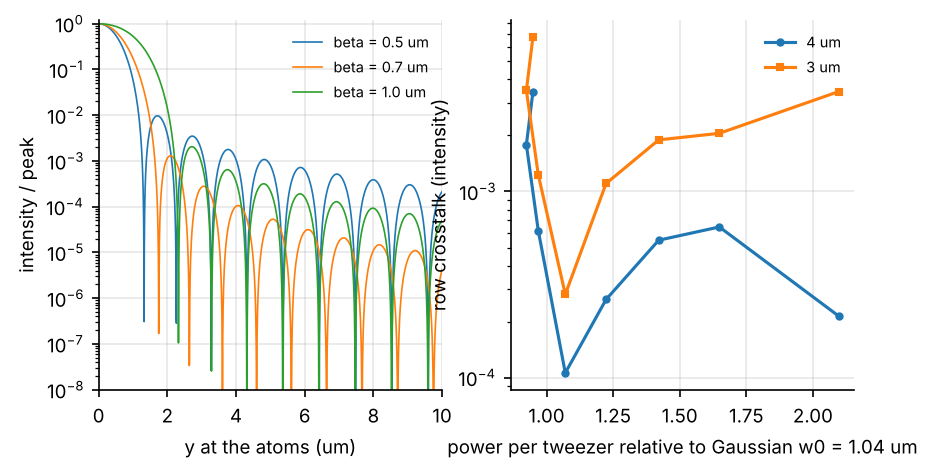
\includegraphics[width=0.85\linewidth]{m13_fill.png}
\caption{Pupil fill and row crosstalk for an ideal FAC (NA~0.9, focal length set by $\beta$, $D=125$),
scalar wave model, 1D in $y$, $s_x=0$ (valid near the row centre, see Sec.~\ref{sec:combine}). Left: $y$
intensity profile at the atoms, normalised to its peak, for $\beta=0.5$, 0.7 and 1.0~\textmu m; the facet far
field is clipped at the collimator aperture and filtered by the NA~0.5 pupil. Right: crosstalk at the
neighbouring row (3 and 4~\textmu m row pitch) against the power per tweezer relative to a Gaussian cross axis
of $w_0=1.04$~\textmu m, for $\beta$ from 0.5 to 1.0~\textmu m. The minimum at power factor 1.07 is
$\beta=0.7$~\textmu m.}
\label{fig:rows-fill}
\end{figure}

At $\beta = 0.7$~\textmu m the $y$ spot is 1.31~\textmu m FWHM, against 1.22~\textmu m for the Gaussian
assumed so far. Together with the 2.7\% cross-axis loss and a 3\% loss to the circular pupil, the power per tweezer rises
by a factor 1.10, the same at the field centre and edge. This raised the power per 1.2~mK tweezer from the
43~mW of the engine design (Gaussian cross axis) to 47~mW. The emitter facet loss found with the real
collimator raises it further, to 57~mW (Sec.~\ref{sec:rows-collimator}).

\subsection{The adopted collimator and the facet loss}\label{sec:rows-collimator}

A collimator must bend rays from $\sin\theta=0.9$ (64$^\circ$ in air) to the axis within a lens no taller
than the 0.5~mm chip pitch, with focal length 175~\textmu m. Single refracting surfaces fail for three
reasons: (i) a plano-hyperbolic lens with its curved side to the facet collimates exactly, but only up to
$\sin\theta=\sqrt{1-1/n^2}$, i.e.\ 0.72 for fused silica and 0.83 for $n=1.8$; (ii) a plano-asphere with its
flat side to the facet reaches NA~0.9, but rays meet its surfaces at up to 43$^\circ$ (fused silica, close to
total internal reflection) or 64$^\circ$ ($n=1.8$, 51\% bare transmission at the flat face); (iii) a single
elliptical surface on a block glued to the facet collimates exactly up to NA $\sqrt{n^2-1}=1.05$, but violates
the sine condition, so that the ray at $s=0.9$ exits at 68\% of the height an aplanatic lens would give.
Here, $s=\sin\theta$ at the facet and $n$ is the lens index.

The Weierstrass construction resolves this. A circular surface of radius $R$ on a glass block, with the facet
at $R/n$ from its centre, is aplanatic: every ray appears to come without aberration from a virtual point, and
the NA drops by $n^2$ (from 0.9 to 0.43 for fused silica). A second lens of focal length
$f_\mathrm{FAC}\,n^2 = 368$~\textmu m then collimates NA~0.43. We design it as a two-asphere aplanat in 2D
(Wassermann-Wolf construction: exact collimation and exact sine condition). A scan of $R$, the air gap, the
aplanat thickness and its index (96 combinations, 29 reaching NA~0.9) selected $R=80$~\textmu m, a
10~\textmu m gap, a 250~\textmu m thick aplanat and $n=1.8$. This combination gives the lowest largest
incidence angle (25.4, 18.2 and 19.2$^\circ$ on the three surfaces). Ray traced, it collimates to NA~0.9 with a
sine-condition error below $4\times10^{-5}$ over the aperture and no residual wavefront error. The lens is
395~\textmu m long (facet to last vertex) with a clear height of $\pm158$~\textmu m. Figure~\ref{fig:rows-designs}
and Table~\ref{tab:rows-designs} compare it with the single-surface alternatives.

\begin{figure}[htbp]\centering
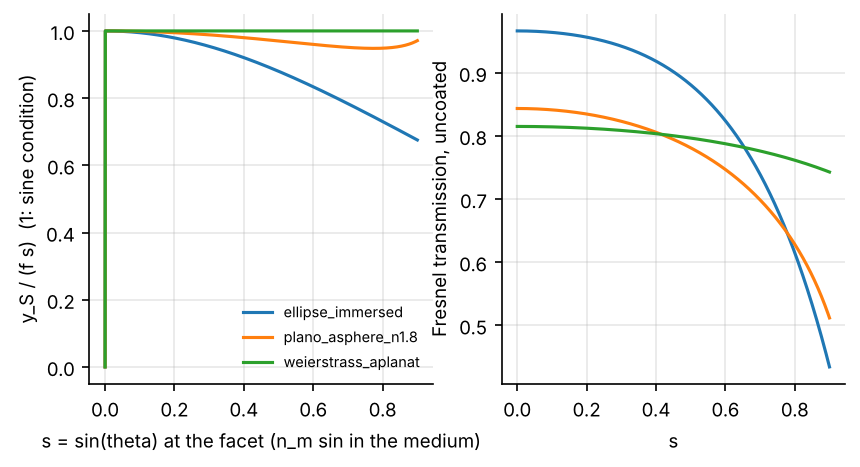
\includegraphics[width=0.85\linewidth]{m14_designs.png}
\caption{Ray-traced collimator designs (2D, cylindrical), focal length 175~\textmu m, NA~0.9. Left: sine
condition, exit height $y_S$ divided by $f\,s$, against the direction sine $s$ at the facet (in the medium for
the glued designs); 1 means aplanatic. Right: Fresnel transmission of the uncoated lens surfaces against $s$.
Designs: ellipse on a glued (immersed) block, plano-asphere of index 1.8 in air, and the adopted Weierstrass
block (fused silica, $R=80$~\textmu m) with a 10~\textmu m gap and a 250~\textmu m aplanat of index 1.8.
The wave model uses AR-coated surfaces.}
\label{fig:rows-designs}
\end{figure}

\paragraph{Facet loss.} The $x$ model of the chip treated the emitter facet as lossless, and the cross-axis
model above normalised to the power radiated into air. A Kirchhoff estimate puts the loss into air at 27\%, from
8\% Fresnel reflection plus the 20\% of the angular spectrum of the 0.39~\textmu m vertical mode that lies
beyond the light cone. We checked this with a 2D FDTD (MEEP, resolution 40/\textmu m) of the vertical
cross-section, with the SiN core index set to 1.965 so that the slab mode index equals that of the 3D mode
(1.7995). Into air, the facet reflects 12.8\% back into the chip and transmits 79.1\%, of which 77.2\% of the
guided power lies within the collimator aperture ($|s|<0.9$; Kirchhoff 72.3\%). Into fused silica, as for the
glued Weierstrass block, it reflects 2.3\% and transmits 95.9\%, with 85.2\% within the aperture (Kirchhoff
82.9\%). The remainder (8\% in air, 2\% in glass) leaves through the cladding near the facet. The emitter facet
thus loses about a quarter of the light into air, a loss absent from all earlier power figures. Gluing the
collimator to the facet recovers about 10\% and cuts the back-reflection sixfold. This is a 2D result with
the lateral confinement folded into the core index; a 3D FDTD of the facet has not been done.

\begin{table}[htbp]\centering\small
\caption{Collimator designs in the wave model (FDTD-scaled facet spectrum, AR-coated lens surfaces, NA~0.5
pupil, $s_x=0$). Peak is per unit guided power relative to the ideal lens in air at $\beta=0.7$~\textmu m.
Power is the laser power per 1.2~mK tweezer, field mean. Simulated.}
\label{tab:rows-designs}
\begin{tabularx}{\linewidth}{Xcccccc}
\toprule
design & sine condition at & largest & $\beta$ & peak & crosstalk at & power per \\
 & $s=0.3$ / 0.6 / 0.9 & incidence & (\textmu m) & & 3 / 4~\textmu m & tweezer \\
\midrule
ideal lens, air & 1 / 1 / 1 & & 0.7 & 1.00 & $2.8\times10^{-4}$ / $1.1\times10^{-4}$ & 61~mW \\
\textbf{Weierstrass + aplanat, glued} & 1.000 / 1.000 / 1.000 & 25$^\circ$ & 0.7 & \textbf{1.10} & $4.0\times10^{-4}$ / $8.0\times10^{-5}$ & \textbf{57~mW} \\
ellipse, printed & 0.954 / 0.834 / 0.675 & 43$^\circ$ & 0.9 & 1.03 & $6.6\times10^{-4}$ / $1.8\times10^{-4}$ & 61~mW \\
ellipse, printed & as above & 43$^\circ$ & 0.7 & 1.22 & $2.1\times10^{-3}$ / $1.0\times10^{-3}$ & \\
plano-asphere $n=1.8$, air & 0.988 / 0.960 / 0.971 & 64$^\circ$ & 0.7 & 1.03 & $4.0\times10^{-4}$ / $1.7\times10^{-4}$ & 59~mW \\
\bottomrule
\end{tabularx}
\end{table}

The aplanatic design reproduces the ideal lens in glass exactly (peak 1.10; a 2D check gives 1.107), with a
$y$ FWHM of 1.35~\textmu m. The ellipse narrows the $y$ spot (1.13~\textmu m at $\beta=0.7$~\textmu m) because
its mapping compresses the outer far field, but the same distortion raises the crosstalk to
$1.0\times10^{-3}$ at 4~\textmu m. Opening the fill to $\beta=0.9$~\textmu m restores $1.8\times10^{-4}$ at a
cost of 15\% in peak. Without AR coatings all designs lose 10 to 30\% ($n=1.8$ surfaces reflect 8\% each at
normal incidence), so coatings are needed in every case. With the adopted collimator the power per 1.2~mK
tweezer is 57~mW, against 47~mW with the facet loss omitted and 61~mW for an ideal lens in air.

\paragraph{The first $x$ lens.} The first lens of the $x$ relay ($f=3.12$~mm, NA~0.355 through the slit)
sees the whole emitter row, $\pm144$~\textmu m, and works off axis. We traced two fused-silica designs from
seven emitter heights and applied each off-axis wavefront to the emitters' angular spectra in the D1 model.
An aplanat has 0.15 waves rms at the 144~\textmu m field (tilt removed). Uncalibrated, its edge tweezer reaches
0.960 of the peak and is shifted by 164~nm; after least-squares recalibration it reaches 1.001 per unit power
with a shift of at most 1.5~nm. A plano-asphere without the sine condition (0.60 waves rms) recovers 0.964 after
recalibration. The static aberration of the $x$ relay is a fixed linear transformation of the chip's response,
and the least-squares synthesis, which already works on the measured response matrix, removes it. The $x$
relay therefore needs ordinary lens quality. The same argument does not apply to the collimator, because the
$y$ axis has no actuators.

\subsection{Crosstalk between rows}\label{sec:rows-crosstalk}

For the 2D test, chip $m$ forms a full row of 41 tweezers at 3~\textmu m spacing over $\pm60$~\textmu m, with
alternating phases 0 and $\pi/2$. The neighbouring chip forms 11 tweezers offset by 1.5~\textmu m in $x$. We
evaluate the pair at row separations of 3 to 16~\textmu m, with the ideal FAC and $s_x=0$. ``Coherent'' means
both chips use one laser frequency, with the worst of eight relative phases; ``incoherent'' means their
relative phase is averaged out. Table~\ref{tab:rows-crosstalk} and Fig.~\ref{fig:rows-crosstalk} give the
results.

\begin{table}[htbp]\centering\small
\caption{Crosstalk between neighbouring rows in 2D (ideal FAC, $\beta=0.7$~\textmu m, $s_x=0$). Full-row
crosstalk is the intensity of a full row of 41 tweezers at the neighbouring row relative to the peak (maximum
over $x$). Static: change of depth / position of a neighbouring tweezer when the full row is switched on.
Moving: change when one tweezer of row $m$ moves by 0.25~\textmu m. Simulated.}
\label{tab:rows-crosstalk}
\begin{tabular}{cccccc}
\toprule
row & full-row & \multicolumn{2}{c}{incoherent rows} & \multicolumn{2}{c}{coherent rows} \\
separation & crosstalk & static & moving & static & moving \\
\midrule
3~\textmu m & $4.3\times10^{-4}$ & $2.0\times10^{-4}$ / 0.13~nm & $6.2\times10^{-5}$ / 0.04~nm & 2.9\% / 18~nm & $6.5\times10^{-3}$ / 5.6~nm \\
4~\textmu m & $1.8\times10^{-4}$ & $1.7\times10^{-4}$ / 0.002~nm & $2.4\times10^{-5}$ / 0.04~nm & 2.6\% / 11~nm & $2.8\times10^{-3}$ / 4.5~nm \\
6~\textmu m & $6.3\times10^{-5}$ & $4\times10^{-6}$ / 0.02~nm & $3\times10^{-6}$ / 0.01~nm & 0.41\% / 8.9~nm & $1.7\times10^{-3}$ / 2.1~nm \\
8~\textmu m & $4.3\times10^{-5}$ & $<10^{-6}$ & $<10^{-6}$ & 0.08\% / 1.8~nm & $1.1\times10^{-3}$ / 1.7~nm \\
12~\textmu m & $1.5\times10^{-5}$ & $<10^{-6}$ & $<10^{-6}$ & 0.01\% / 5.9~nm & $8\times10^{-4}$ / 0.8~nm \\
16~\textmu m & $1.3\times10^{-5}$ & $2\times10^{-6}$ & $<10^{-6}$ & 0.27\% / 1.6~nm & $4\times10^{-4}$ / 0.6~nm \\
\bottomrule
\end{tabular}
\end{table}

\begin{figure}[htbp]\centering
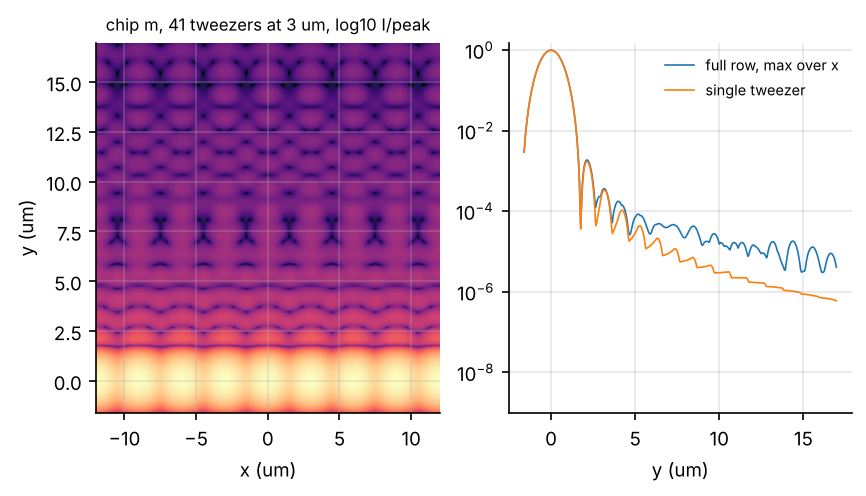
\includegraphics[width=0.85\linewidth]{m13_crosstalk.png}
\caption{Light from one chip at the neighbouring rows, 2D scalar model with D1's beam-propagation response in
$x$ and the facet mode through an ideal NA~0.9 FAC in $y$ ($\beta=0.7$~\textmu m, $s_x=0$, valid near the row
centre). Left: $\log_{10}$ of the intensity relative to the peak for a full row of 41 tweezers at
3~\textmu m spacing, alternating phases 0 and $\pi/2$, shown over $|x|\le12$~\textmu m. Right: maximum over
$x$ of the full row's intensity against $y$, compared with a single tweezer. The full row has a tail plateau
of about $10^{-5}$ out to 16~\textmu m.}
\label{fig:rows-crosstalk}
\end{figure}

With incoherent rows, a moving tweezer changes the next row by at most $6\times10^{-5}$ in depth and
0.04~nm in position, even at 3~\textmu m row pitch. This is two orders of magnitude below the in-row figures of
D1 (0.11\%, 3.5~nm). With coherent rows, the crosstalk field $\epsilon$ (in intensity) interferes with the
neighbour's own field, so the depth changes by about $2\sqrt{\epsilon}\cos\phi$. Here, $\phi$ is the relative
optical phase of the two chip feeds. This interference persists at all simulated distances because of the
tail plateau of a full row. Its strength follows $\phi$, which drifts with temperature and acoustics in the
separate fibre paths, so the 2.6\% and 11~nm at 4~\textmu m become slow, uncontrolled noise. Alternating two
frequencies between neighbouring chips is therefore not enough. In the original plan of the study every chip
ran at its own frequency, with pairwise differences of at least 1~MHz, far above twice the 84~kHz trap
frequency: one acousto-optic shifter per chip feed at $80 + 1.13\,m$~MHz ($m=0$ to 15), each handling 2.6 to
3.4~W (handling at this power: [VALUE?]). The beat notes then modulate the depth at MHz rates with amplitude
about $2\sqrt{\epsilon}$, which the atoms average. The next subsection replaces these 16 shifters. The tweezers
within one row stay coherent in either scheme, as the least-squares synthesis of the engine requires.

\subsection{Decorrelating the rows without frequency shifters}\label{sec:rows-decorrelate}

A frequency offset $\delta f$ makes $\phi$ advance at $2\pi\,\delta f$, and the atom sees only the time
average when $\delta f$ is far above the trap frequencies. Any process that randomises $\phi$ on time scales
much shorter than the trap period does the same. We use a common random phase seen with different delays. If
the seed carries a phase $\varphi(t)$ and chip $m$ receives it after a delay $\tau_m$, the relative phase of
chips $m$ and $n$ is $\varphi(t-\tau_m)-\varphi(t-\tau_n)$. Its mean contribution to the interference is the
field coherence $|\langle \exp\{i[\varphi(t)-\varphi(t-\tau)]\}\rangle|$ at $\tau=\tau_m-\tau_n$.

Our choice of modulation is a compromise between residual coherence and tolerance to real hardware. A binary
$0/\pi$ m-sequence ($N=1023$) leaves $9.8\times10^{-4}=1/N$ at integer delays. However, every transition passes
through $+\pi/2$, so a modulator with a 10--90\% rise of 0.3 bit leaves a carrier of 0.12 and a residual
coherence of $4.1\times10^{-2}$, and a depth error of 5\% (10\%) gives $5.2\times10^{-3}$
($2.4\times10^{-2}$). A Zadoff-Chu polyphase code ($N=1021$) has perfect autocorrelation but needs exact delays
($6.2\times10^{-2}$ at non-integer ones). Gaussian phase noise of $\sigma=3$~rad rms needs neither: the carrier
is $\exp(-\sigma^2/2)$, and any delay longer than about three correlation times decorrelates. Its residual
coherence is $1.2\times10^{-4}$ in the ensemble ($\exp(-9)$), and 4.2 to $7.2\times10^{-3}$ in our
32,768-bit simulated records, which is their statistical floor. What the atom sees is set by the low-frequency
density of the interference term, $0.40/B$, where $B$ is the correlation rate of the noise. For the coherent
term $2\sqrt{\epsilon}=2.1\times10^{-2}$ this gives a relative intensity noise density
$S_I(2\nu_\mathrm{trap})=8.8\times10^{-14}$/Hz at $B=2$~GHz. The parametric heating rate
$\Gamma=\pi^2\nu^2 S_I(2\nu)$ \cite{OHARA} is then $6\times10^{-3}$~s$^{-1}$ at $\nu=84$~kHz, an energy
e-folding time above 2 minutes; at $B=0.5$~GHz it is $2.4\times10^{-2}$~s$^{-1}$.

The adopted scheme is therefore one fibre-coupled LiNbO$_3$ phase modulator on the low-power seed, ahead of the
1:16 split, driven by a Gaussian noise source amplified to about $1\,V_\pi$ rms (3~rad) over 1 to 2~GHz. The
16 chip feeds receive 0, 0.3, 0.6, \ldots, 4.5~m of extra fibre (steps of at least three correlation lengths at
2~GHz). Within one chip and its relay, path differences are at most about 1~mm (about 5~ps). With a 0.5~ns
correlation time and $\sigma=3$~rad the coherence loss is $\sigma^2(\tau/\tau_c)^2/2\approx5\times10^{-4}$,
so the synthesis sees an essentially coherent source. The optical spectrum becomes Gaussian with rms width
$0.67B$ (1.35~GHz, 5~pm, at $B=2$~GHz). Through the diffractive objective's axial chromatic shift
(16~\textmu m/nm, derived for $f_\mathrm{obj}\propto1/\lambda$) this smears the focus by 0.08~\textmu m rms
(peak 0.9998) and the lateral position at 60~\textmu m by 0.29~nm rms. The spectrum is symmetric, so the mean
light shift at the double-magic wavelength is unchanged to first order; the second-order term needs the
curvature of the differential polarisability, which we do not have [VALUE?]. A seed broadened to about 1~GHz
also raises the stimulated-Brillouin threshold of the high-power amplifier and the delivery fibres, which
carry about 3~W each ([REF?]; recalled: SBS suppression by phase modulation is standard in high-power
single-frequency fibre amplifiers). If the chosen amplifier already broadens its seed for this reason, the only
addition is the fibre delays. Compared with 16 acousto-optic shifters, the scheme removes 16 RF drivers and the
shifter insertion loss (about 15\% each [VALUE?]).

\begin{table}[htbp]\centering\small
\caption{Options for row independence: perturbation of a tweezer by all other rows within $\pm16$~\textmu m
(both sides; rms over drifting relative phases, pairs in quadrature; 4~\textmu m rows, full rows of 41
tweezers; $s_x=0$). Criteria used for tweezers within a chip: others' depth change $<3\times10^{-3}$ and
position change $<5$~nm when a tweezer moves; position noise budget of the proposal 10~nm rms. Simulated
(vector focusing for the polarisation options) and derived.}
\label{tab:rows-options}
\begin{tabularx}{\linewidth}{lXccc}
\toprule
option & added hardware & power & static: depth / position & moving 0.25~\textmu m: depth / position \\
\midrule
all chips coherent & none & 1 & 2.3\% / 9.2~nm & $2.3\times10^{-3}$ / 5.1~nm \\
per-chip frequency offsets & 16 shifters at 2.6 to 3.4~W & 1 (+ shifter loss) & $1.8\times10^{-4}$ / 0.09~nm & $2\times10^{-5}$ / 0.05~nm \\
\textbf{phase noise + delays} & \textbf{1 modulator on the seed, noise source, $\le5$~m fibre} & \textbf{1} & $\mathbf{1.6\times10^{-4}}$ / \textbf{0.07~nm} & $\mathbf{2\times10^{-5}}$ / \textbf{0.04~nm} \\
alternating $x$/$y$ polarisation & half-wave-plate strips (passive) & 1 & $4.2\times10^{-3}$ / 2.5~nm & $1.1\times10^{-3}$ / 1.6~nm \\
$y$ apodiser, $a=0.65$ & graded mirror (passive) & 1.84 & $5.2\times10^{-3}$ / 4.1~nm & $1.0\times10^{-3}$ / 1.8~nm \\
polarisation + apodiser $a=0.8$ & passive & 1.55 & $2.8\times10^{-3}$ / 1.8~nm & $5.7\times10^{-4}$ / 0.7~nm \\
\bottomrule
\end{tabularx}
\end{table}

As can be seen from Table~\ref{tab:rows-options}, common phase noise with fibre delays gives the same row
independence as per-chip frequency offsets, at no power penalty. Leaving all chips coherent breaks the
position budget: 9.2~nm rms of slow wander plus 5.1~nm when neighbours move.

\paragraph{Passive alternatives.} A half-wave-plate strip in front of every other chip, in the collimated region
after the collimators, gives alternate rows orthogonal linear polarisation. Vector focal fields (Richards-Wolf,
aplanatic NA~0.5 objective, intensity summed over $E_x$, $E_y$ and $E_z$) show that the interference of
orthogonal neighbours falls by a factor of 26; the residual comes from the depolarisation of high-angle rays,
mainly via $E_z$. Rows two apart (8~\textmu m) share a polarisation and then dominate. The moving-tweezer
criteria and the position budget are met, but the static depth wanders by 0.4\% rms with the fibre phases at
Hz to kHz rates. The option has three costs: (i) the meta-objective must be polarisation-insensitive
(propagation-phase meta-atoms with fourfold symmetry rather than geometric phase); (ii) where the orthogonal
fields overlap, the polarisation becomes elliptical in proportion to their relative phase, which produces a
vector light shift. With a vector-to-scalar ratio of about $0.09\,g_F m_F$ per unit ellipticity (recalled, to
be verified, from the far-detuned formula \cite{GRIMM}) and an ellipticity of up to about $2\times10^{-2}$ at
4~\textmu m, this is about $2\times10^{-3}\,g_F m_F$ of the trap depth: up to tens of kHz for stretched states
and zero to first order for clock states ($m_F=0$); (iii) only two orthogonal states exist, so rows two apart
stay coherent. A passive Gaussian apodiser at the $y$ telescope plane conjugate to the pupil lowers the 1D
crosstalk at 4~\textmu m from $8.4\times10^{-5}$ to $3.5\times10^{-6}$ ($a=0.65$ pupil radii), but it costs a
factor 1.84 in power, widens the $y$ spot from 1.35 to 1.73~\textmu m, and in 2D still leaves
$4.7\times10^{-3}$ of static depth change at 4~\textmu m. It is not competitive. We adopt the phase noise with
fibre delays. Alternating polarisation costs nothing to add and gives a second, independent factor of about 26
on the nearest rows if the modulation fails or is switched off.

\subsection{Conversion of phase noise to intensity noise}\label{sec:rows-pmam}

Phase noise alone leaves the intensity constant (the simulated control gives $-376$~dB/Hz, the numerical
floor). Intensity noise appears only where an element filters the spectrum. We simulated each element of a
laser chain separately on the modulated field ($\sigma=3$~rad, $B=2$~GHz; record 131~\textmu s at 16~GS/s; for
delayed copies, the worse of two relative phases). The criterion is a parametric heating rate
$\Gamma\le0.1$~s$^{-1}$ at $\nu=84$~kHz (energy doubling time about 7~s), i.e.\ a relative intensity noise
(RIN) density at 168~kHz of $S\le1.4\times10^{-12}$/Hz ($-118$~dB/Hz). Table~\ref{tab:rows-pmam} gives the
results.

\begin{table}[htbp]\centering\small
\caption{Phase-to-intensity conversion by individual elements of the laser chain (Gaussian phase noise
3~rad rms, $B=2$~GHz). RIN rms is over all frequencies (mostly at GHz); the density is at 168~kHz $=2\nu_\mathrm{trap}$.
Element parameters are chosen ranges, not component data; PM-fibre group delay 1.2~ps/m and dispersion
20~ps$^2$/km are recalled, to be verified. Simulated.}
\label{tab:rows-pmam}
\begin{tabularx}{\linewidth}{Xccc}
\toprule
element & RIN rms & RIN at 168~kHz & $\Gamma$ (s$^{-1}$) \\
\midrule
amplifier gain tilt, 0.05 / 0.5 / 5~dB/nm & $6\times10^{-5}$ / $6\times10^{-4}$ / $6\times10^{-3}$ & $-237$ / $-216$ / $-182$~dB/Hz & $<10^{-6}$ \\
band-pass 1~nm FWHM, offset 250~pm (ASE filter) & $7\times10^{-3}$ & $-173$~dB/Hz & $<10^{-6}$ \\
band-pass 100~pm, centred / offset 25~pm & $1.0\times10^{-2}$ / $7.0\times10^{-2}$ & $-130$ / $-133$~dB/Hz & $7\times10^{-3}$ / $3\times10^{-3}$ \\
band-pass 30~pm, centred / offset 7.5~pm & $9.6\times10^{-2}$ / 0.21 & $\mathbf{-110}$ / $\mathbf{-113}$~dB/Hz & \textbf{0.70} / \textbf{0.37} \\
multipath $R_1=R_2=10^{-2}$, delay $\ge0.3$~ns & $1.4\times10^{-2}$ & $-130$~dB/Hz & $7\times10^{-3}$ \\
multipath $R_1=R_2=10^{-2}$, delay 0.1 / 0.01~ns & $7\times10^{-3}$ / $10^{-4}$ & $-133$ / $-171$~dB/Hz & $3\times10^{-3}$ / $10^{-6}$ \\
multipath $R_1=R_2=10^{-3}$ or $10^{-4}$, any delay & $\le1.4\times10^{-3}$ & $\le-149$~dB/Hz & $\le8\times10^{-5}$ \\
PM fibre, extinction $-20$~dB, 5 / 20~m, then TE guide & $3\times10^{-4}$ / $5\times10^{-3}$ & $-161$ / $-137$~dB/Hz & $6\times10^{-6}$ / $1.4\times10^{-3}$ \\
dispersion, 5~m to 1~km & $\le8\times10^{-4}$ & $<-280$~dB/Hz & 0 \\
representative chain & $6.9\times10^{-3}$ & $-134.5$~dB/Hz & $2.5\times10^{-3}$ \\
\bottomrule
\end{tabularx}
\end{table}

The structure follows from the physics. Gain tilt and dispersion respond to the instantaneous frequency, the
time derivative of the phase, whose spectrum vanishes towards low frequency, so their intensity noise lies at
GHz. A delayed copy of amplitude $r$ produces an intensity term $2r\cos[\varphi(t)-\varphi(t-\tau)]$. Once
$\tau$ exceeds the correlation time (about 0.3~ns), this term is a random, telegraph-like signal of variance
$2r^2$ spread over about $B$, so $S\approx4r^2\times0.40/B$ (Fig.~\ref{fig:rows-pmam}). For $\tau$ far below
the correlation time the term is quadratic in the phase increment and much smaller. A band-pass filter
narrower than the spectrum acts as the same effect distributed over its impulse response, about
$1/(\pi\,\mathrm{FWHM}) = 40$~ps for 30~pm. The dependence on $B$ cuts both ways: at $r=10^{-2}$ and
$\tau=1$~ns, $S$ is $-125$, $-130$ and $-138$~dB/Hz for $B=0.5$, 2 and 8~GHz, whereas at $\tau=0.1$~ns
$B=0.5$~GHz is the quietest ($-170$~dB/Hz) because the copy still lies inside the correlation time. We keep
$B=2$~GHz as a middle value.

\begin{figure}[htbp]\centering
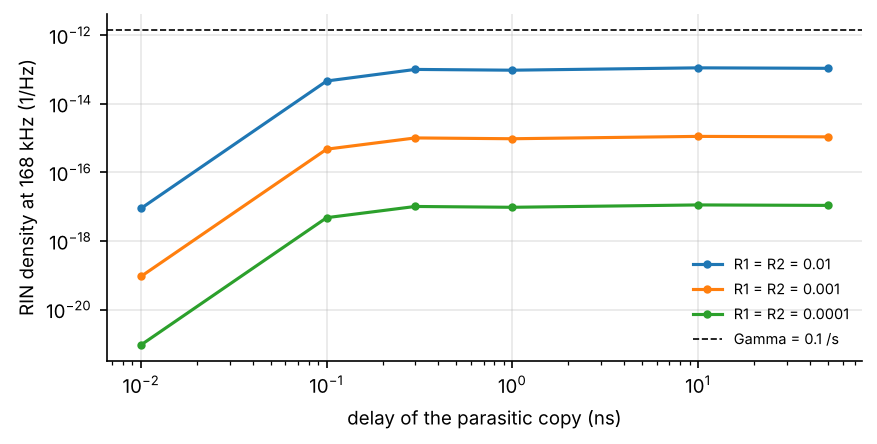
\includegraphics[width=0.8\linewidth]{m16_pm_am.png}
\caption{RIN density at 168~kHz ($2\nu_\mathrm{trap}$) produced by one parasitic delayed copy from two
reflections $R_1=R_2$, against the delay of the copy, for Gaussian phase noise of 3~rad rms at $B=2$~GHz
(simulated record 131~\textmu s at 16~GS/s, worse of two relative phases). Dashed line: the criterion
$\Gamma=0.1$~s$^{-1}$ at $\nu=84$~kHz ($1.4\times10^{-12}$/Hz). Beyond about 0.3~ns the density saturates at
$\approx4r^2\times0.40/B$ with $r^2=R_1R_2$.}
\label{fig:rows-pmam}
\end{figure}

Two design rules follow: (i) no filter narrower than about 100~pm (20 times the 1.35~GHz rms modulation width)
in the light path; (ii) the product of any two reflections in the chain below $R_1R_2=1.7\times10^{-3}$
(amplitude $r\le0.042$), i.e.\ no pair of uncoated glass surfaces in series. A representative chain (amplifier
tilt 0.5~dB/nm; ASE filter of 1~nm FWHM offset by 250~pm; 5~m of PM fibre with $-20$~dB polarisation
crosstalk; two $-30$~dB connector reflections 5~m apart; an on-chip etalon between a $-30$~dB input facet and
the 2.3\% glued emitter facet, 190~ps round trip; 5~m of dispersion) gives $-134.5$~dB/Hz and
$\Gamma=2.5\times10^{-3}$~s$^{-1}$ (energy e-folding about 7~min), 16~dB inside the criterion. The on-chip
etalon and the connector pair dominate. Without modulation, the same reflections produce no noise at 168~kHz.
Instead they give a slow intensity offset $2r\cos\Phi$ that follows the drift of the path phase $\Phi$: 2\% for
$r=10^{-2}$, at Hz to kHz rates. The modulation converts this offset into broadband noise of the same rms, of
which only $10^{-13}$ to $10^{-12}$/Hz lands near the trap frequencies. The phase noise therefore also helps
against parasitic etalons, provided rule (ii) holds. The elements are linear and treated separately; amplifier
gain dynamics, self-phase modulation and stimulated Brillouin scattering are not modelled. The prediction to
test is a RIN floor below $-130$~dB/Hz at 10~kHz to 1~MHz after the full amplified chain, with a 1~nm ASE
filter and AR-coated components, with the modulation on and off.

\subsection{Alignment, assembly and drift}\label{sec:rows-align}

Table~\ref{tab:rows-tol} gives per-chip errors for a single tweezer at $x=0$ with the ideal collimator (the
field edge, $x=60$~\textmu m, gives the same values within 0.1\% at $s_x=0$). None of these errors moves the
row in $y$ by more than 0.01~nm.

\begin{table}[htbp]\centering\small
\caption{Alignment tolerances of one chip and its FAC (ideal collimator, 2D, $s_x=0$). Peak is at the nominal
atom plane relative to no error; crosstalk is the worst value at the 4~\textmu m neighbour (no error:
$1.1\times10^{-4}$, $y$ FWHM 1.33~\textmu m). Simulated.}
\label{tab:rows-tol}
\begin{tabular}{lccc}
\toprule
error & value & peak & crosstalk at 4~\textmu m \\
\midrule
FAC decentre in $y$ & 0.05 / 0.1 / 0.2 / 0.3~\textmu m & 0.992 / 0.969 / 0.881 / 0.750 & $2\times10^{-4}$ / $4\times10^{-4}$ / $1.2\times10^{-3}$ / $2.8\times10^{-3}$ \\
FAC focus along $z$ & 0.25 / 0.5 / 1 / 2~\textmu m & 0.993 / 0.973 / 0.893 / 0.641 & $3\times10^{-4}$ / $9\times10^{-4}$ / $2.8\times10^{-3}$ / $4.3\times10^{-3}$ \\
FAC roll about $z$ & 0.5 / 1 / 2~mrad & 0.998 / 0.992 / 0.968 & $10^{-4}$ / $10^{-4}$ / $2\times10^{-4}$ \\
smile (bow, peak to valley) & 0.1 / 0.2 / 0.4~\textmu m & 0.998 / 0.992 / 0.967 & $10^{-4}$ / $2\times10^{-4}$ / $4\times10^{-4}$ \\
FAC wavefront, spherical-like & 0.05 / 0.1 waves rms & 0.942 / 0.783 & $3\times10^{-4}$ / $1.2\times10^{-3}$ \\
FAC wavefront, coma-like & 0.05 / 0.1 waves rms & 0.937 / 0.767 & $5\times10^{-4}$ / $2.0\times10^{-3}$ \\
chip piston along $z$ & 10 / 100 / 300~\textmu m & $\ge0.999$ / $\ge0.992$ / $\ge0.908$ & \\
\bottomrule
\end{tabular}
\end{table}

The collimator decentre is the tightest tolerance: $\pm0.1$~\textmu m for 3\% loss. A decentre $\delta$ shifts
the facet image in the pupil by $\delta/\beta$ of the pupil radius, so the tolerance scales with the vertical
facet mode. It costs power and crosstalk but does not move the row. The ray-traced designs confirm that it is a
property of the facet, not of the lens: $\pm0.1$~\textmu m for every design (peak 0.973 at 0.1~\textmu m and
0.896 at 0.2~\textmu m for the adopted collimator). Focus is looser for the glued designs because the facet
radiates into glass (the defocus phase scales as $n_m\cos\theta$, with $n_m$ the medium index): about
$\pm1$~\textmu m for 3\% for the adopted collimator, against $\pm0.5$~\textmu m for the ideal lens in air. The
wavefront requirement (about 0.03 waves rms for $\le3\%$ at NA~0.9) follows from the same imaging: the collimator
is the aperture of the facet-to-pupil image, and light it scatters out of that image misses the pupil. For the
adopted collimator this translates into a surface form error of at most 20~nm rms for $\le2\%$ loss (mean peak
0.984 at 20~nm and 0.916 at 50~nm rms, correlation length 20~\textmu m). A chip piston of 10, 100 and 300~\textmu m
moves the $x$ position statically by at most 1.5, 0.9 and 6.8~nm, so facets must stay flush to within about
100~\textmu m. Stair-step stacking for wire bonds is therefore excluded, and fibre and electrical access must
come from the chip sides or back; this access is not addressed here.

The row positions at the atoms follow from the conjugations (derived). A height error of chip plus collimator,
or a placement error of the collimator, moves its row by $1/D = 8$~nm per \textmu m. A chip tilt about $x$ of
1~mrad moves the row by $f_\mathrm{FAC}\times1~\mathrm{mrad}/D=1.4$~nm. A chip piston $\mathrm{d}z$ defocuses
its row in $y$ by $\mathrm{d}z/D^2$ (6~nm per 100~\textmu m). A stack built to $\pm2$~\textmu m therefore places
rows to $\pm16$~nm; a static offset of this size must be matched by the static 1075~nm array, or measured and
absorbed into its design.

Drift sets the mounting. For a collimator glued to its own facet, vertical registration is fixed at the facet,
and differential expansion acts only over the lens's own height ($\pm80$~\textmu m at the glued block). With
$\Delta\alpha\approx2\times10^{-6}$/K (Si $2.6\times10^{-6}$/K against fused silica $0.55\times10^{-6}$/K,
recalled, to be verified) this is about 0.2~nm/K. A monolithic collimator array for the whole stack, referenced
at its base, would see the full 8~mm stack height: 16~nm/K at the top chip, so 0.1~\textmu m after 6~K. Hence
one collimator per chip, or a stack held to $\pm1$~K. Thermal expansion of the Si stack itself moves the outer
rows by about 0.2~nm/K at the atoms. The glue line of the immersed design lies along $z$, so cure shrinkage
changes mainly the focus ($\pm1$~\textmu m tolerance) and only weakly the decentre; the vertical position must
nevertheless be held to $\pm0.1$~\textmu m during cure, and the shrinkage and creep of UV adhesives at this level
need a source [REF?]. The alignment signal is strong: a decentre moves the facet image across the pupil by
$\delta\times12{,}400$, so 0.1~\textmu m becomes 1.2~mm on the 17~mm pupil, and a camera with 10~\textmu m pixels
imaging the pupil (or its conjugate in the $y$ telescope) resolves 1~nm of decentre in principle. Active
alignment against this signal, before and during cure, is the process we recommend. A collimator printed by
two-photon lithography directly on the facet would be registered lithographically; its placement accuracy
needs a source [REF?], as do the achievable wavefront error of NA~0.9 micro-collimators [REF?] and the
long-term stability of actively aligned, bonded collimators [REF?].

\subsection{Power and laser plan for 16 chips}\label{sec:rows-power}

Table~\ref{tab:rows-power} gives the power plan with the adopted collimator (57~mW per 1.2~mK tweezer, field
mean, FDTD-scaled facet, AR-coated lenses), for 192-port chips (Sec.~\ref{sec:moretweezers}) with 45 tweezers
per row at 4~\textmu m spacing or 60 at 3~\textmu m.

\begin{table}[htbp]\centering\small
\caption{Laser power for 16 chips with the adopted collimator, and input fibres per chip at a facet intensity
cap of 20~MW/cm$^2$ (a design choice; no damage threshold was found). Derived.}
\label{tab:rows-power}
\begin{tabular}{cccccc}
\toprule
tweezers per row & depth & power per chip & 16 chips & \multicolumn{2}{c}{fibres per chip} \\
 & & & & lensed tip & HI1060-matched tip \\
\midrule
45 (4~\textmu m) & 1.2~mK & 2.6~W & 41~W & 5 & 1 (8~MW/cm$^2$) \\
60 (3~\textmu m) & 1.2~mK & 3.4~W & 55~W & 6 & 1 (11~MW/cm$^2$) \\
45 & 0.5~mK & 1.1~W & 17~W & 2 & 1 \\
60 & 0.5~mK & 1.4~W & 23~W & 3 & 1 \\
\bottomrule
\end{tabular}
\end{table}

Our choice of one input fibre per chip is a compromise between two considerations. First, the lensed-fibre
inverse taper of the input coupler study has a 3.1~\textmu m$^2$ mode at the chip facet, so the 20~MW/cm$^2$ cap
allows only 0.62~W per fibre and 5 to 6 fibres per chip. Several inputs would split the 128 ports into
sub-trees whose relative optical phases drift with their fibres, and a tweezer window straddling a sub-tree
boundary would then fluctuate. However, the HI1060-matched taper (tip 0.1~\textmu m, $-0.48$~dB, 0.11~dB worse
than the lensed tip) has a 30.6~\textmu m$^2$ mode and carries 6.1~W at the same cap. One fibre per chip is
therefore possible and preferred, at the cost of a 0.1~\textmu m tip width that sits at the assumed minimum
feature size. With 16 rows the stack offers 720 (4~\textmu m spacing) to 960 (3~\textmu m) independent
tweezers. The laser must deliver 41 to 55~W of single-frequency 1064.4~nm light at 1.2~mK, or 17 to 23~W at
0.5~mK; the availability of 40 to 55~W is a placeholder [VALUE?]. Lowering the
transport depth is the cheapest lever, because power scales linearly with depth and the lower trap frequency
also relaxes the required update rate (Secs.~\ref{sec:moretweezers} and~\ref{sec:transport}).

The limits of this section are as follows. The model is scalar, with ideal (sine-condition) thin cylindrical
lenses for the relay; the objective's apodisation factor and polarisation are omitted except in the vector
calculation of the polarisation option. The collimator ray trace is 2D, with ideal AR coatings in the wave
model, and the $n=1.8$ glass is a class, not a catalogue glass. The facet FDTD is 2D with an effective core
index. Tolerances are evaluated one at a time; a combined Monte Carlo of decentre, focus, form, thickness and
index has not been run. All $y$ results assume $s_x=0$ and hold near the row centre only
(Sec.~\ref{sec:combine}).

\section{More tweezers per engine and per row}\label{sec:moretweezers}

This section asks how many independent tweezers one engine can carry, what limits the number, and how a stack
of engines can serve more sites than it has tweezers. The packing results are simulated on the
beam-propagation matrix of design D1, the star-coupler aberration with exact path lengths, and the transport
depths with a 1D classical Monte Carlo; the scaling tables are derived from these
(\texttt{docs/scaling.md}, \texttt{docs/scaling\_beyond.md}).

The answer in brief: the useful number of tweezers per row is the row length divided by the site pitch, and
the row length is set by the diffraction-limited field of the objective. A 192-port chip filling the
$\pm100$~\textmu m field of the proposal carries 45 tweezers on the 4~\textmu m site lattice and needs 383 fast
actuators. Sixteen such chips in the stacked relay of Sec.~\ref{sec:rows} give 720 simultaneous tweezers, and a
row-select tilt lets this one stack serve all 50 rows of the field, 2,250 sites, in four passes. The
per-tweezer costs, 8.7 fast actuators and about 57~mW at 1.2~mK, do not fall with scale. For comparison, the
1,024-atom assembly with crossed acousto-optic deflectors cited in the proposal moved a median of 13 (maximum 38)
atoms in parallel \cite{proposal}.

\subsection{Packing within a row}\label{sec:moretweezers-packing}

We filled the $\pm60$~\textmu m row of D1 with tweezers at spacing $s$, neighbours in phase quadrature, and
synthesised the port amplitudes by least squares. Table~\ref{tab:more-packing} and
Fig.~\ref{fig:more-packing} give the result. The peak per tweezer per unit port power stays at 0.256 from 6
to 2.5~\textmu m spacing, so the power per tweezer is independent of how many are lit. At 3~\textmu m the
barrier between neighbours is 78\% of the trap depth, which keeps the atoms separate; at 2.5~\textmu m the
independence degrades to the 1\% level, and at 2~\textmu m the spots merge. We take 3~\textmu m (2.8
resolution cells, or 1.75 spot widths) as the practical packing limit. It is set by the spot width
(1.71~\textmu m FWHM), hence by the NA: at fixed NA, a narrower spot needs a less apodised window, which raises
the tails.

\begin{table}[htbp]\centering\small
\caption{Packing a $\pm60$~\textmu m row of design D1 (beam-propagation matrix, least-squares synthesis,
neighbours in phase quadrature). Simulated.}
\label{tab:more-packing}
\begin{tabular}{ccccc}
\toprule
spacing & tweezers & intensity midway & others' change when & residual after \\
 & & between neighbours & one moves 0.25~\textmu m & switch-off \\
\midrule
6~\textmu m & 21 & $5\times10^{-4}$ & 0.11\%, 1.6~nm & $<10^{-5}$ \\
4~\textmu m & 31 & 3.8\% & 0.10\%, 2.6~nm & $10^{-5}$ \\
3~\textmu m & 41 & 22\% & 0.11\%, 3.3~nm & $9\times10^{-4}$ \\
2.5~\textmu m & 49 & 43\% & 0.79\%, 10~nm & $9\times10^{-3}$ \\
2~\textmu m & 61 & 76\% (spots merge) & 5.2\%, 74~nm & $7\times10^{-2}$ \\
\bottomrule
\end{tabular}
\end{table}

\begin{figure}[htbp]\centering
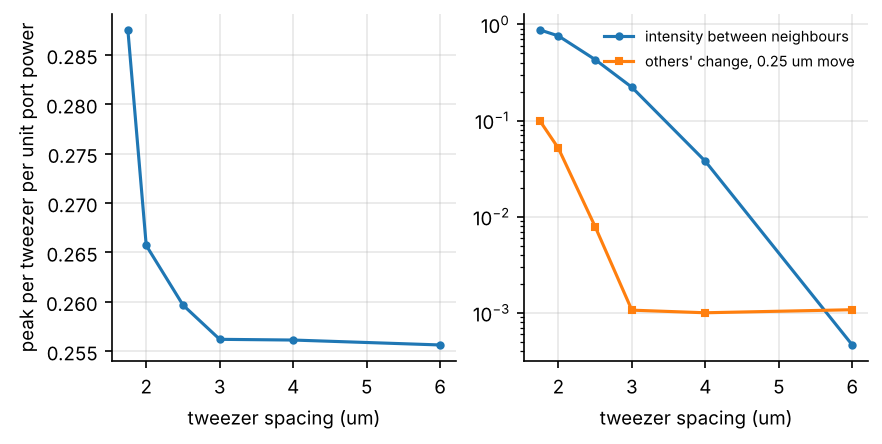
\includegraphics[width=0.85\linewidth]{m12_packing.png}
\caption{Packing limit of one engine, simulated on the beam-propagation response matrix of design D1 (128
ports, NA~0.5, 1064.4~nm) with least-squares synthesis of a $\pm60$~\textmu m row. Left: peak intensity per
tweezer per unit port power against tweezer spacing; it is flat at 0.256 from 6 to 3~\textmu m and rises only
as the spots merge. Right: intensity midway between neighbours (relative to the peak) and the largest change
of the other tweezers' depth when one tweezer moves by 0.25~\textmu m. Below 3~\textmu m the independence
degrades rapidly.}
\label{fig:more-packing}
\end{figure}

However, the proposal places atoms on a 4~\textmu m site lattice. The 41 tweezers of D1 at 3~\textmu m spacing
then reduce to 30 useful ones over the same $\pm60$~\textmu m. In general a row of length $L$ holds $L/4+1$
tweezers on 4~\textmu m sites, so the number per row cannot be raised by packing more densely. Scaling
therefore means longer rows and more rows.

\subsection{Ports per engine: field, actuators, power and slab}\label{sec:moretweezers-ports}

Each input port adds one resolution cell (1.06~\textmu m at NA~0.5) to the row. A row of $L$ thus needs $L/1.06$
ports, which is 3.8 ports and 7.5 to 8.7 fast actuators per tweezer, independent of $L$.
Table~\ref{tab:more-scaling} scales the engine with 1.5$\times$ oversampled arms, 2.0~\textmu m slab pitch and
1.5~\textmu m emitter pitch. The binding limits, in order, are (i) the objective field, (ii) the number, speed
and accuracy of the fast actuators, (iii) the laser power through each chip and (iv) the slab size. The
star-coupler aberration is not a limit below about 512 ports.

\begin{table}[htbp]\centering\small
\caption{Scaling of one focal-plane engine (1.5$\times$ oversampled arms, 2.0~\textmu m slab pitch,
1.5~\textmu m emitter pitch; row field 88\% of the port field). Fast actuators: two per port; data rate at
200~kHz and 16 bit. Aberration: worst-port rms arm-phase error on the Rowland circle (geometric lower bound).
Derived from the simulated packing and aberration results.}
\label{tab:more-scaling}
\begin{tabular}{cccccccc}
\toprule
ports & row field & tweezers at & slab radius & fast & static & data rate & aberration \\
 & & 4 / 3~\textmu m & / area & actuators & trims & & (rms) \\
\midrule
128 & 136~\textmu m & 30 / 40 & 1.3~mm / 0.5~mm$^2$ & 255 & 192 & 0.8~Gbit/s & 0.03~rad \\
\textbf{192} & \textbf{204~\textmu m} & \textbf{45 / 60} & \textbf{2.0~mm / 1.1~mm$^2$} & \textbf{383} & \textbf{288} & \textbf{1.2~Gbit/s} & \textbf{0.05~rad} \\
256 & 272~\textmu m & 60 / 80 & 2.7~mm / 2.0~mm$^2$ & 511 & 384 & 1.6~Gbit/s & 0.07~rad \\
512 & 545~\textmu m & 120 / 160 & 5.3~mm / 8.2~mm$^2$ & 1023 & 768 & 3.3~Gbit/s & 0.13~rad \\
1024 & 1090~\textmu m & 240 / 320 & 10.6~mm / 33~mm$^2$ & 2047 & 1536 & 6.6~Gbit/s & 0.27~rad \\
\bottomrule
\end{tabular}
\end{table}

\paragraph{Objective field.} The row can only be as long as the objective's diffraction-limited field. The
$\pm100$~\textmu m meta-objective target of the proposal corresponds to about 192 ports. Longer rows need a
larger corrected field at NA~0.5, which is the hardest optical requirement in the system. Refractive plan
objectives of NA~0.5 have flat fields of several hundred micrometres (recalled, to be verified). With a
$\pm250$~\textmu m field, 480 ports would give 110 tweezers per row, at a slab radius of about 5~mm and an
aberration of about 0.12~rad. A larger corrected field is the only route to longer rows.

\paragraph{Fast actuators.} Two per port: 383 for a 192-port row, each updated at $\ge200$~kHz (the
transport-heating limit at 1.2~mK) and accurate to about 1\% in amplitude and 10~mrad in phase for 10~nm
position noise. Beyond a few hundred channels per chip this needs drivers flip-chip bonded or co-integrated
with the photonics, and closed-loop calibration (on-chip power taps or camera feedback) against PZT hysteresis
and drift. This is the main engineering limit.

\paragraph{Power.} Power is linear in the number of simultaneous tweezers and in the depth. The engine design
gave 43~mW per 1.2~mK tweezer; the cross axis and the emitter facet loss raise this to 57~mW with the glued
collimator (factor 1.34, Sec.~\ref{sec:rows-collimator}). A full 192-port row of 45 tweezers then needs 2.6~W at
1.2~mK. An earlier plan to feed a row through 2 to 3 fibres into separate sub-trees is superseded: one
HI1060-matched input fibre per chip carries this power below the facet intensity cap
(Sec.~\ref{sec:rows-power}).

\paragraph{Slab and aberration.} The slab radius grows linearly with the port count (2~mm at 192 ports, 5~mm at
512). This fits within one die but exceeds a single electron-beam writing field, so stitching errors must be
absorbed by the static trims, or the slab written by DUV lithography. With the arm envelope produced by the
synthesis, the worst-port residual phase error grows linearly with size, about $0.033~\mathrm{rad}\times(\text{ports}/128)$
on the Rowland circle (port arc of radius $R/2$, Fig.~\ref{fig:more-aberration}). A quartic correction of the
port curve gains nothing, so the remainder comes from the circular arm arc; an aspheric arm curve would be the
next step beyond about 512 ports. These geometric values are about half the beam-propagation figure for D1
(0.079~rad), so they are lower bounds. Even doubled, they keep the Strehl ratio above 0.93 up to 512 ports.

\begin{figure}[htbp]\centering
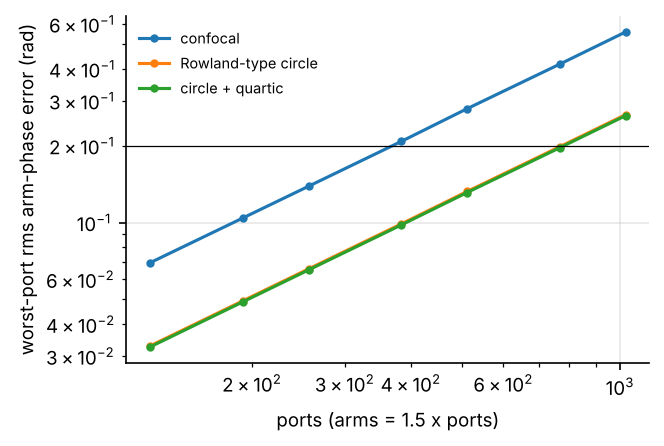
\includegraphics[width=0.65\linewidth]{m12_aberration.png}
\caption{Worst-port rms arm-phase error of the star coupler against the number of input ports (arms
$=1.5\times$ ports), computed from exact path lengths with the arm envelope of the least-squares synthesis, for
a confocal layout, a Rowland-type circle and a circle with quartic correction of the port curve. The
horizontal line marks 0.2~rad. The Rowland-type layout scales as about $0.033~\mathrm{rad}\times(\text{ports}/128)$;
the quartic correction adds nothing. Geometric values; the beam-propagation figure for D1 is about twice as
large.}
\label{fig:more-aberration}
\end{figure}

\paragraph{The 192-port chip.} We choose 192 ports because this matches the row to the $\pm100$~\textmu m field
of the proposal (a $\pm90$~\textmu m row on 4~\textmu m sites) and stays well inside the slab and aberration
limits (2.0~mm, 0.05~rad). It carries 45 tweezers on the site lattice (60 at the 3~\textmu m packing limit) with
383 fast actuators, 288 static trims and a data rate of 1.2~Gbit/s. The row length assumed here exceeds what
the adopted cylindrical collimator serves in the stacked relay: for D1, skew rays limit a row to
$|x_a|\le45$~\textmu m with the best common focus offset (Sec.~\ref{sec:rows-fill}). The counts below assume full
rows; Sec.~\ref{sec:combine} treats the skew-ray limit.

\subsection{Rows, stacks and row select}\label{sec:moretweezers-stack}

One engine addresses one row, and one chip with its collimator aligned to 0.1~\textmu m makes one row of the
stacked relay (Sec.~\ref{sec:rows}). We take 8 to 16 rows as the practical stack size; this is an engineering
judgement by analogy with laser-diode stacks, not a result. Sixteen chips make an 8~mm stack and 64~\textmu m of
rows, against a 200~\textmu m field.

\paragraph{Row select.} The pupil of the $y$ relay is conjugate to every chip's facet, and the atom plane to the
collimators' focal plane $S$. A tilt at any plane conjugate to the pupil therefore translates all rows of the
stack rigidly in $y$, without aberration in the paraxial limit. Shifting the 16 rows by 64~\textmu m is a
3.7~mrad tilt at the objective pupil. At the internal Fourier plane of the $y$ telescope, where the beam is 21.6
times smaller, it is 80~mrad optical, i.e.\ a 40~mrad mechanical rotation of a mirror about 1~mm tall in $y$
and about 20~mm wide. Placing rows to 10~nm needs about 6.5~\textmu rad of mechanical repeatability, which is
galvanometer-scanner class (recalled, to be verified against a specific scanner). Translating the whole stack
by 8~mm with 1~\textmu m accuracy is a slower alternative (1~\textmu m becomes 8~nm at the atoms). Atoms wait
in the static 1075~nm array between passes. A 16-chip stack then serves all 50 rows of the
$\pm100$~\textmu m field, 2,250 sites, in four passes, and the hardware per site drops by a factor 3.1. The same
tilt moves all rows of the stack together, so the stack can carry atoms in 2D: independently along $x$ within
each row, and in common along $y$. The scheduling of such passes is treated in Sec.~\ref{sec:rearrange}.

\paragraph{A second stack.} A polarising beam splitter before the objective combines a second 16-chip stack,
orthogonally polarised and offset by 64~\textmu m so the stacks never overlap. This doubles the simultaneous
capacity (32 rows, two passes) at twice the hardware, so the cost per tweezer is unchanged. It needs a
polarisation-insensitive objective, as does the polarisation option of Sec.~\ref{sec:rows-decorrelate}.
Table~\ref{tab:more-config} summarises the configurations.

\begin{table}[htbp]\centering\small
\caption{Configurations at 4~\textmu m site pitch (192-port chips except the first row; 57~mW per 1.2~mK
tweezer). Derived. Transport at lower depth reduces the power, see text.}
\label{tab:more-config}
\begin{tabular}{lcccccc}
\toprule
configuration & simultaneous & sites & passes & chips & fast & power at \\
 & tweezers & served & & & actuators & 1.2~mK \\
\midrule
one D1 chip (128 ports) & 30 & 30 & 1 & 1 & 255 & 1.7~W \\
one 192-port chip ($\pm90$~\textmu m row) & 45 & 45 & 1 & 1 & 383 & 2.6~W \\
stack of 16 & 720 & 720 & 1 & 16 & 6,128 & 41~W \\
\textbf{stack of 16 + row select} & \textbf{720} & \textbf{2,250} & \textbf{4} & \textbf{16} & \textbf{6,128} & \textbf{41~W} \\
two stacks (orthogonal pol.) + row select & 1,440 & 2,250 & 2 & 32 & 12,256 & 83~W \\
\bottomrule
\end{tabular}
\end{table}

\paragraph{Transport depth.} The 1.2~mK depth of the proposal is what fast long moves need: a 40~\textmu m move
in 100~\textmu s survives only at 1.2~mK even with a smooth trajectory, and with a 200~kHz staircase it does not
survive at any simulated depth, because each update step (up to 3.75~\textmu m) exceeds the 1.43~\textmu m
waist. Shorter or slower moves need much less depth. In a 1D classical Monte Carlo (4,000 atoms at
10~\textmu K, Gaussian potential with $w=1.43$~\textmu m, minimum-jerk trajectory, 200~kHz staircase), the
minimum depth for a loss $\le10^{-3}$ and an energy gain of at most one trap quantum per move is 0.2~mK for a
12~\textmu m (three-site) move in 200~\textmu s and 0.5~mK for a 40~\textmu m (ten-site) move in
200~\textmu s. For 12~\textmu m it is 0.8~mK at 100~\textmu s and 0.1~mK at 400~\textmu s; for 40~\textmu m no
depth up to 1.2~mK suffices at 100~\textmu s, and 0.2~mK does at 400~\textmu s. The excitation is
not monotonic in depth, because at some depths the trap frequency aliases with the update steps. This first
estimate cut the power of 720 tweezers from 41~W to 6.9 to 17~W. The 3D simulation with handoff to and from the
static array (Sec.~\ref{sec:transport}) has since revised it. The moving trap must be at least three times the
static hold depth, the hold about $20\,k_BT$, and moves must run along lanes between the rows. The minimum
moving depth is therefore 0.3~mK for 5~\textmu K atoms (0.6~mK for 10~\textmu K), not 0.2~mK, which gives 10
to 21~W for 720 tweezers (17 to 34~W for 1 to 2~\textmu K heating per move). Rearrangement mostly needs short
moves; a cycle of four passes at about 0.6~ms each (pick-up and release ramps assumed at 100~\textmu s each, a
200~\textmu s move and 200~\textmu s for the $y$ tilt to settle) takes 2 to 3~ms, and the depth can be raised for
the occasional long move.

\subsection{What does not work}\label{sec:moretweezers-not}

Three routes to more tweezers per chip fail. (i) Packing tweezers below the site pitch adds nothing on a
4~\textmu m lattice (Sec.~\ref{sec:moretweezers-packing}). (ii) Several emitter rows per chip cannot be
separated at the atoms: rows a few \textmu m apart on the facet land within nanometres of each other, and a separate collimator per emitter row cannot be fitted. (iii) Spectral
multiplexing of rows through the dispersive star coupler is excluded by the objective's chromatic focal shift
of 16~\textmu m/nm.

One untested route may remove the stack altogether: planar tiling of surface-emitting chips (speculative, not
simulated). Chips placed side by side on a common carrier, each with long grating emitters, would be imaged in
$y$ onto the atoms with demagnification $D$ = tile pitch/4~\textmu m, i.e.\ $D=1500$ for a 6~mm tile pitch. The
object-side NA in $y$ is then $3.3\times10^{-4}$, which a 2~mm weak grating radiates directly, so no collimator
is needed, and chip placement errors shrink by $D$ (10~\textmu m becomes 7~nm). The 0.1~\textmu m decentre
tolerance is replaced by an emission-angle tolerance of about 30~\textmu rad, i.e.\ $\delta n_\mathrm{eff}\sim3\times10^{-5}$,
trimmable with a heater (about 1.5~K) or by tilting the chip. The open questions are the grating efficiency
(emission up and down) and fitting the engine (slab of about 2~mm) and a 2~mm grating within one tile. Scaling
of these building blocks to $10^4$ to $10^6$ sites, with blocks of engines and the walls set by static
trapping power, the objective field and the 3~\textmu m lane distance, is the subject of
Sec.~\ref{sec:megascale}.

\section{Transport and handoff in three dimensions}\label{sec:transport}

This chapter tests whether a moving tweezer of the adopted design can lift an atom out of a static trap, carry it across the array and hand it to an empty static trap without losing it, heating it, or disturbing the atoms it passes. With the moving-trap field computed through the real optical chain and a static array of Gaussian traps, a 12 or 40~\textmu m move delivers 3,000 of 3,000 simulated atoms (loss $<10^{-3}$ at 95\% confidence) under three conditions: (i) the move runs along a lane between the rows, not along a row; (ii) the moving depth is at least three times the static hold depth; (iii) the hold depth is about $20\,k_BT$. Here, $k_BT$ is the thermal energy of the atoms. With slow handoff steps (200~\textmu s ramps, 400~\textmu s lane steps) the heating per move falls to 0.12 to 0.16~\textmu K at a moving depth of only 0.3~mK, in both a one-dimensional quantum and a three-dimensional classical model, so the shallow, low-power operating point is also the low-heating point. The one tight alignment is the axial registration of the 1064.4 and 1075~nm foci. A lattice with 3~\textmu m pitch along the rows and 4~\textmu m between rows transports as cleanly as the $4\times4$~\textmu m lattice.

These results revise two earlier estimates. The one-dimensional transport model of the scaling study, which left out the handoff, the static array and the third dimension, gave a minimum moving depth of 0.2~mK; once handoff and waiting atoms are included this is too optimistic. The first three-dimensional operating points, with 100~\textmu s steps, heated the atom by 1 to 10~\textmu K per move; the slower steps of Sec.~\ref{sec:transport-timing} remove most of this heating.

\subsection{Model}\label{sec:transport-model}

The moving trap is the intensity of one tweezer of design D1 (beam-propagation response, least-squares synthesis), passed through the Weierstrass and aplanat collimator and the circular NA 0.5 pupil, and computed by scalar focusing with defocus on a grid of $7\times6\times20$~\textmu m. Its full widths at half maximum are 1.73~\textmu m along the row ($x$), 1.37~\textmu m across it ($y$) and 9.8~\textmu m along the axis ($z$); at 1~mK its trap frequencies are 54, 67 and 22~kHz. We hold its shape fixed while it moves and sample its position and depth at 200~kHz. The static array consists of Gaussian beams at 1075~nm with a waist of 0.85~\textmu m (our choice) and a Rayleigh range of 2.1~\textmu m, at 4~\textmu m pitch, in three rows of 15 sites. All sites share one global hold depth, since a fixed meta-optic array cannot switch single sites. The two wavelengths add incoherently.

The atoms are classical Cs atoms, integrated by velocity Verlet with 0.25~\textmu s steps and gravity along $y$, with 1,500 to 3,000 atoms per case. Each starts in a thermal distribution sampled in the harmonic approximation and truncated to atoms bound in the real Gaussian site. The sequence is: ramp the moving trap up on the source site ($\sin^2$, 100~\textmu s); step 2~\textmu m in $y$ into the lane (100~\textmu s); move in $x$ with a minimum-jerk profile; step back to the row (100~\textmu s); ramp down on the target site (100~\textmu s); hold for 100~\textmu s. An atom counts as delivered if it is bound in the target static trap after the moving trap is off. The lane lies halfway between rows 4~\textmu m apart, which puts it as far as possible from the waiting atoms on both sides.

\subsection{Lanes between the rows}\label{sec:transport-lanes}

A tweezer that moves along its own row passes over empty static sites. The total potential then develops a dip that travels with the moving trap and kicks the atom. Losses depend strongly on the move time, with resonances where the transit time over one site matches the trap period (Table~\ref{tab:transport-row}). At most settings 45 to 95\% of the atoms are lost. Only a moving trap five times deeper than the static traps, moving slowly (400~\textmu s), recovers 99.1 to 99.7\%, and then at 14 to 24~\textmu K of heating.

\begin{table}[htbp]\centering\small
\caption{Fraction of atoms delivered when the 12~\textmu m move runs along the row, over empty static sites, for two move times (simulated, classical, 1,500 atoms per case).}
\label{tab:transport-row}
\begin{tabular}{lll}
\toprule
hold / moving depth & move in 200~\textmu s & move in 400~\textmu s \\
\midrule
0.1 / 0.3~mK & 5 to 7\% & 54 to 57\% \\
0.1 / 0.5~mK & 42 to 48\% & 99.1 to 99.7\% (heating 14~\textmu K) \\
0.2 / 0.5~mK & 11\% & 99.3 to 99.6\% (heating 24~\textmu K) \\
\bottomrule
\end{tabular}
\end{table}

Along a lane 2~\textmu m off the row, reached with the row-select $y$ tilt, the static traps have fallen to $1.6\times10^{-5}$ of their depth and transport is clean. The lane costs one shared $y$ tilt per pass (100~\textmu s each way), which the row-select mirror already provides. Because the tilt is shared, all tweezers of a stack enter and leave the lanes together; this is the main constraint the scheduler of Sec.~\ref{sec:rearrange} must respect.

\subsection{Depth ratio, hold depth and temperature}\label{sec:transport-depth}

The ratio of moving to hold depth decides whether the handoff completes. At a ratio of 1.5, 5\% of the atoms stay behind in the source site; at 2, 3 to 5\% are lost; at 3, 99.5 to 99.9\% are delivered with about 10~\textmu K of heating per move; at 5, 99.6 to 100\% are delivered with 1 to 2.6~\textmu K (all with 100~\textmu s steps).

The hold depth is set by the atoms that wait next to a lane. They feel the out-of-focus light of the passing tweezer, which at 1.5 to 2.5~\textmu m from its axis and a few micrometres from focus is 6 to 15\% of its peak intensity. At a hold depth of $10\,k_BT$, 1 to 2\% of these waiting atoms are lost from the hot tail of the distribution; at $20\,k_BT$, none of 3,000. Table~\ref{tab:transport-op} lists the resulting operating points. The required depth is set by the atom temperature, not by the move: about $60\,k_BT$ for the moving trap, or $100\,k_BT$ for low heating with fast steps. Cooling the atoms from 10 to 5~\textmu K therefore halves the laser power.

\begin{table}[htbp]\centering\small
\caption{Operating points for a 12~\textmu m move in 400~\textmu s along a 2~\textmu m lane, with 100~\textmu s ramps and lane steps and 200~kHz updates (simulated, classical, 3,000 atoms). Power per tweezer is derived by scaling 57~mW at 1.2~mK with depth; the second number is for 720 tweezers.}
\label{tab:transport-op}
\setlength{\tabcolsep}{3.5pt}
\begin{tabular}{llllll}
\toprule
atoms & hold / moving & delivered & heating per move & waiting lost & power, 1 / 720 tweezers \\
\midrule
5~\textmu K & 0.1 / 0.3~mK & 3000/3000 & 9.9~\textmu K & 0/3000 & 14~mW / 10~W \\
5~\textmu K & 0.1 / 0.5~mK & 3000/3000 & 1.8~\textmu K & $\le$2/3000 & 24~mW / 17~W \\
10~\textmu K & 0.2 / 0.6~mK & 3000/3000 & 10.0~\textmu K & 0/3000 & 29~mW / 21~W \\
10~\textmu K & 0.2 / 1.0~mK & 3000/3000 & 0.9~\textmu K & $\le$3/3000 & 48~mW / 34~W \\
\bottomrule
\end{tabular}
\end{table}

\subsection{Step timing and heating per move}\label{sec:transport-timing}

The classical model is not reliable when the energy gain is near one trap quantum (about 1 to 3~\textmu K here). We therefore check the handoff with a one-dimensional split-step propagation along $y$, the handoff and lane axis. The atom starts in the ground state of the static site; the $y$ profile of the moving tweezer is taken from the three-dimensional grid, and gravity is included. The $x$ move is treated separately. We compare with classical trajectories from a Wigner sample of the same ground state (Table~\ref{tab:transport-quantum}).

\begin{table}[htbp]\centering\small
\caption{Energy gain per handoff along $y$ (source ramp, lane step out and back, target ramp) from 1D split-step propagation, the fraction of atoms left in the ground state, and the classical gain from a Wigner sample of the same initial state (simulated). The trap quantum of the static site is 1.4~\textmu K at 0.1~mK and 2.0~\textmu K at 0.2~mK.}
\label{tab:transport-quantum}
\begin{tabular}{lllll}
\toprule
hold / moving & ramp / lane step & gain, quantum & ground state kept & gain, classical \\
\midrule
0.1 / 0.3~mK & 100 / 100~\textmu s & 9.7~\textmu K & 0.08 & 11.6~\textmu K \\
0.1 / 0.3~mK & 100 / 200~\textmu s & 2.0~\textmu K & 0.21 & 1.4~\textmu K \\
0.1 / 0.3~mK & 200 / 400~\textmu s & 0.12~\textmu K & 0.98 & 0.94~\textmu K \\
0.1 / 0.5~mK & 100 / 100~\textmu s & 0.84~\textmu K & 0.84 & 1.53~\textmu K \\
0.1 / 0.5~mK & 200 / 400~\textmu s & 0.13~\textmu K & 0.99 & 0.87~\textmu K \\
0.2 / 0.6~mK & 200 / 400~\textmu s & 0.15~\textmu K & 0.99 & 1.72~\textmu K \\
0.2 / 1.0~mK & 100 / 100~\textmu s & 1.58~\textmu K & 0.66 & 1.58~\textmu K \\
\bottomrule
\end{tabular}
\end{table}

The $x$ move adds 0.08 to 0.37~\textmu K in both models, with 0.98 to 0.99 of the ground state kept. Two findings follow. First, the lane step, not the $x$ move, sets the heating, and the heating falls steeply with the step duration: from 100 to 400~\textmu s the gain at 0.1/0.3~mK drops 80-fold. Second, above about one trap quantum the classical model agrees with the quantum one to within a factor of 2, on the pessimistic side; below it, Wigner sampling overstates the heating by up to a factor of 10, as expected for zero-point motion. A three-dimensional classical run with the slow steps confirms delivery of 3,000 of 3,000 atoms, with 0.16~\textmu K of heating for 5~\textmu K atoms at 0.1/0.3~mK and 0.59~\textmu K for 10~\textmu K atoms at 0.2/0.6~mK, and no loss of waiting atoms.

Hence three step timings are available, and the choice between them is a trade between heating and cycle time (Sec.~\ref{sec:rearrange}). The slow steps (200~\textmu s ramps, 400~\textmu s lane steps) heat by 0.12 to 0.16~\textmu K per handoff at 0.3~mK, or 0.2 to 0.3~\textmu K per move once the $x$ move is included. The intermediate steps (100~\textmu s ramps, 200~\textmu s lane steps) heat by about 2~\textmu K per move. The fast steps (100~\textmu s lane steps) heat by about 10~\textmu K at a moving depth of 0.3~mK, or 1.2~\textmu K at 0.5~mK. The slow, cold regime needs the least laser power; the fast regime at 0.5~mK shortens the cycle at the cost of 24 instead of 14~mW per tweezer (Table~\ref{tab:transport-op}).

\subsection{Alignment and depth tolerances}\label{sec:transport-tol}

Table~\ref{tab:transport-tol} lists the fraction delivered under misalignments and timing changes. Three points follow. (i) Axial registration of the two foci is the one tight alignment, to about $\pm1$~\textmu m for delivery. A diffractive objective shifts focus by about 170~\textmu m between 1064.4 and 1075~nm (16~\textmu m/nm, derived), so the two paths must be focused independently before they are combined, and then held. (ii) Lateral registration is loose: 0.4~\textmu m costs nothing, so the 16~nm row-placement budget of the stacked relay is not a constraint for transport. (iii) Speed is not limiting in this regime: 40~\textmu m in 400~\textmu s is as safe as 12~\textmu m.

\begin{table}[htbp]\centering\small
\caption{Tolerances of the handoff: fraction of 10~\textmu K atoms delivered at a hold depth of 0.1~mK, 12~\textmu m in 400~\textmu s along the lane, 100~\textmu s steps, unless the row states otherwise (simulated, classical).}
\label{tab:transport-tol}
\setlength{\tabcolsep}{3.5pt}
\begin{tabular}{llll}
\toprule
parameter & values & moving 0.3~mK & moving 0.5~mK \\
\midrule
nominal & & 0.9993 & 0.9993 \\
axial focus offset & 0.5 / 1 / 2 / 4~\textmu m & 0.998 / 0.995 / 0.939 / 0.455 & 0.995 / 0.997 / 0.957 / 0.902 \\
lateral offset, $y$ & 0.1 / 0.2 / 0.4~\textmu m & 1.000 / 0.998 / 0.999 & 1.000 / 1.000 / 0.998 \\
lateral offset, $x$ & 0.1 / 0.2 / 0.4~\textmu m & 0.998 / 1.000 / 0.998 & 1.000 / 1.000 / 0.999 \\
ramp time & 25 / 200~\textmu s & 0.994 / 0.998 & 0.993 / 1.000 \\
move & 40~\textmu m in 400 / 800~\textmu s & 0.998 / 0.998 & 0.998 / 1.000 \\
updates & smooth, not 200~kHz & 0.999 & 0.999 \\
gravity & off & 0.999 & 0.999 \\
\bottomrule
\end{tabular}
\end{table}

Delivery is not the tightest criterion for the axial offset; heating is. We propagate the axial motion in one dimension from the ground state of the static site (axial trap quantum 0.40~\textmu K at 0.1~mK), with the static depth following the lateral separation of the moving-trap centre and the moving trap's axial profile taken from the three-dimensional grid. Here, $\delta z$ is the axial offset between the 1075 and 1064~nm foci. With coincident foci the axial motion is not excited, because the change of axial trap frequency during the handoff is adiabatic. A focus offset displaces the axial equilibrium twice per move, and that is what heats (Table~\ref{tab:transport-axial}). With the slow steps, keeping the axial heating below the lateral 0.12 to 0.15~\textmu K needs $|\delta z|\le0.5$~\textmu m; 1~\textmu m costs about 2~\textmu K per move and 2~\textmu m costs 4 to 8~\textmu K. This tightens the $\pm1$~\textmu m delivery tolerance into a heating tolerance of $\pm0.5$~\textmu m, or 0.3\% of the chromatic focal offset. A slow stage on the last $y$ and $x$ lenses of the relay, calibrated on the atoms, would provide the adjustment; an active focus lock between the two paths is the corresponding hardware requirement.

\begin{table}[htbp]\centering\small
\caption{Axial energy gain per move versus the axial focus offset $\delta z$ (1D split-step propagation; the classical Wigner values agree to within 20\% above 1~\textmu K and are pessimistic below).}
\label{tab:transport-axial}
\begin{tabular}{llllll}
\toprule
hold / moving & ramp / lane step & $\delta z=0$ & 0.5~\textmu m & 1~\textmu m & 2~\textmu m \\
\midrule
0.1 / 0.3~mK & 100 / 100~\textmu s & 0.06~\textmu K & 4.1~\textmu K & 16.6~\textmu K & 40.7~\textmu K \\
0.1 / 0.3~mK & 200 / 400~\textmu s & $<0.01$~\textmu K & 0.19~\textmu K & 2.0~\textmu K & 8.3~\textmu K \\
0.1 / 0.5~mK & 100 / 100~\textmu s & 0.02~\textmu K & 6.4~\textmu K & 31.0~\textmu K & 28.3~\textmu K \\
0.1 / 0.5~mK & 200 / 400~\textmu s & $<0.01$~\textmu K & 0.22~\textmu K & 1.8~\textmu K & 4.4~\textmu K \\
\bottomrule
\end{tabular}
\end{table}

The depth uniformity of the static array, in contrast, is not a constraint. With lane transport, 2,000 atoms per case and the three operating points 5~\textmu K at 0.1/0.3~mK, 5~\textmu K at 0.1/0.5~mK and 10~\textmu K at 0.2/0.6~mK, a source site deeper by 20, 40 or 60\% still delivers at least 0.996, a target site shallower by a factor 0.8, 0.6 or 0.4 at least 0.998, and random depth errors of 5, 10 or 20\% rms deliver 1.000 in all cases. This is far beyond the errors a meta-optic or SLM array would show.

\subsection{Denser lattices: 3~\textmu m pitch}\label{sec:transport-pitch}

At 3~\textmu m pitch in both directions, the lane between rows is only 1.5~\textmu m from the waiting atoms. The moving tweezer, 1.37~\textmu m wide across the row and with strong out-of-focus light, then captures them (Table~\ref{tab:transport-pitch}, upper part; slow steps, 3,000 atoms). The transported atom is always delivered, but at 0.1/0.3~mK only 0.335 of the waiting atoms in the same row stay and 0.584 are lost. A square 3~\textmu m lattice would therefore need empty corridor rows, which cost most of the density gain: a repeating layout of computation row, corridor and reservoir row gives (1/3)/9~\textmu m$^{-2}$ = 0.037~\textmu m$^{-2}$ computation sites, only about 20\% above 0.031~\textmu m$^{-2}$ at 4~\textmu m with a 1:1 reservoir layout.

However, only the closest approach to the waiting atoms matters, and that is set by the lane, not by the pitch along the row. A $3\times4$~\textmu m lattice (3~\textmu m along the rows, rows 4~\textmu m apart, lane 2~\textmu m) therefore transports as cleanly as $4\times4$~\textmu m (Table~\ref{tab:transport-pitch}, lower part). It has 33\% more sites per area: 0.063 against 0.047 computation sites per \textmu m$^2$ with a 3:1 reservoir layout. This supersedes the earlier conclusion that 3~\textmu m pitch needs corridors; that conclusion holds only for a 3~\textmu m row spacing. Corridor rows 6~\textmu m apart with a 3~\textmu m lane are also safe (3000/3000 delivered, 0.3 to 1.5~\textmu K, no waiting atom lost at all three operating points), but less dense.

\begin{table}[htbp]\centering\small
\caption{Transport at 3~\textmu m pitch (simulated, classical, 3,000 atoms per case, 200~\textmu s ramps and 400~\textmu s lane steps). Upper part: square 3~\textmu m lattice with a 1.5~\textmu m lane; fraction of waiting atoms that stay in the same row next to the lane and in the next row beside the drop. Lower part: $3\times4$~\textmu m lattice with a 2~\textmu m lane; waiting atoms lost among the in-row neighbour at 3~\textmu m, the atoms passed by the lane and the next row beside the drop, out of 3,000.}
\label{tab:transport-pitch}
\begin{tabular}{llll}
\toprule
hold / moving (atoms) & delivered & heating & waiting atoms \\
\midrule
\multicolumn{4}{l}{\textit{square 3~\textmu m lattice, lane 1.5~\textmu m: fraction that stays, same row / next row}} \\
0.1 / 0.3~mK & 1.000 & & 0.335 / 0.149 (0.584 / 0.851 lost) \\
0.1 / 0.5~mK & 1.000 & & 0.001 / 0.006 \\
0.2 / 0.6~mK & 1.000 & & 0.225 / 0.117 \\
0.2 / 1.0~mK & 1.000 & & 0.014 / 0.012 \\
\midrule
\multicolumn{4}{l}{\textit{$3\times4$~\textmu m lattice, lane 2~\textmu m: number lost, in-row neighbour / passed by lane / next row}} \\
0.1 / 0.3~mK (5~\textmu K) & 3000/3000 & 0.16~\textmu K & 0 / 0 / 0 \\
0.1 / 0.5~mK (5~\textmu K) & 3000/3000 & 0.05~\textmu K & 0 / 0 / 3 of 3000 \\
0.2 / 0.6~mK (10~\textmu K) & 3000/3000 & 0.59~\textmu K & 0 / 0 / 0 \\
\bottomrule
\end{tabular}
\end{table}

The intermediate steps are also clean on the dense lattice. With 100~\textmu s ramps, 200~\textmu s lane steps and 300~\textmu s moves over 9~\textmu m along the lane, 3,000 of 3,000 atoms are delivered with 3.0~\textmu K of heating per move at 0.1/0.3~mK (5~\textmu K atoms) and 0.8~\textmu K at 0.2/0.6~mK (10~\textmu K atoms), and no bystander at 3~\textmu m, at 6~\textmu m or in the next row is lost or displaced. This is consistent with the 2.0~\textmu K of the quantum check (Table~\ref{tab:transport-quantum}), and we use 2~\textmu K per move for this timing in the steady-state analysis of Sec.~\ref{sec:megascale}.

\subsection{Limits}\label{sec:transport-limits}

The three-dimensional model is classical, and the quantum check is one-dimensional per axis, with the atom assumed to sit at the moving-trap centre laterally for the axial check. Light-assisted processes, photon scattering by the trapping light (a few photons per second at 0.3 to 0.5~mK, estimated from the far-detuned rate, not simulated) and the vector light shift are not included. The moving trap's shape is assumed invariant along the row; least-squares synthesis keeps it within 0.1\%, but the traced collimator of the later design study defocuses tweezers away from the row centre, which this model does not include. Neighbouring tweezers in the same row (independent tweezers 4~\textmu m away) are not included, and the static traps are ideal Gaussian beams. The loss per move is not computed: 0 of 3,000 atoms bounds it below about $10^{-3}$, and smaller values used in Sec.~\ref{sec:rearrange} are assumptions.

\section{Rearrangement and repair}\label{sec:rearrange}

This chapter turns the single moves of Sec.~\ref{sec:transport} into a full rearrangement cycle, counts its passes, time and moves per atom, and asks what limits the probability of a defect-free block. A 16-chip stack with row select assembles a defect-free $32\times32$ block from a $50\times45$ array loaded at 50\% in 17.2~ms on average over 40 loadings (worst 23.0~ms), with 5.8 balancing and 2 compaction passes. Every loading succeeded before losses were applied. The average atom in the block moves 1.12 times and none moves more than twice, so with the slow handoff steps the finished block is no more than about 0.6~\textmu K hotter than at the start. One round of imaging and repair then takes 10 to 13~ms. The outcome is set by losses, not by the scheduler: by the loss per move, the loss per image and the vacuum lifetime. The photonic chip contributes 1.1 moves per atom and 17~ms per cycle; reaching a 99\% defect-free block requires each loss term near $10^{-5}$, which is a property of the platform.

\subsection{Hardware rules and scheduler}\label{sec:rearrange-scheduler}

The hardware sets three rules: (i) a stack addresses 16 consecutive rows at a time; (ii) every tweezer of the stack shares the $y$ motion (into the lane 2~\textmu m off the row, optionally along mid-column lanes over $j$ rows, and back), while each tweezer moves independently in $x$; (iii) tweezers in one row keep their order and so stay at least 4~\textmu m apart. The scheduler works in two stages. In vertical balancing, each pass chooses a stack position $k$ and a common row shift $j$ that move the most surplus atoms into target rows lacking atoms. Arriving atoms go straight to empty target columns where possible, and atoms that arrive in a pass are not picked again in the same pass. In horizontal compaction, one pass per group of 16 target rows matches each row's atoms in order to the target columns and pushes the extras just outside the block.

A pass takes two ramps, two lane steps, the $x$ moves (minimum jerk, 400~\textmu s per 40~\textmu m, scaled as $\sqrt{d}$ with the distance $d$, at least 200~\textmu s), the $y$ travel for $j$ rows, and 0.3~ms of scanner settling (our choice). Of the 2.2~ms of a typical pass, ramps, lane steps and settling make up 1.3~ms. The schedule is greedy and not optimal: a planner that combines balancing and compaction, or shares passes between stack positions, would need fewer passes. Section~\ref{sec:rearrange-modes} shows how much better pass selection gains.

\subsection{Cycle time and moves per atom}\label{sec:rearrange-cycle}

Table~\ref{tab:rearrange-cycle} lists the cycle for several targets and loadings, and Fig.~\ref{fig:rearrange-cycle} shows the mean cycle time. A larger target from the same $50\times45$ array costs more balancing passes ($36\times36$ at 60\% needs 8.3 + 3 and 25.1~ms on average), while a higher loading saves them (32$\times$32 at 60\%: 14.8~ms). A second stack, combined with the first to address 32 rows, does not change the number of balancing passes but saves one compaction pass (15.5 against 17.2~ms for the $32\times32$ block at 50\%). The number of moves per atom stays near 1.1 in every case: about 22\% of the atoms in the $32\times32$ block at 50\% loading move twice, the rest once or not at all.

\begin{table}[htbp]\centering\small
\caption{One rearrangement cycle from a $50\times45$ array, mean over 40 random loadings, base timing (100~\textmu s ramps, 400~\textmu s lane steps, 0.3~ms settling); passes are vertical (V, balancing) plus horizontal (H, compaction). Defects are expected numbers in the block, from the assumed loss per move (moves) and from vacuum loss during the cycle at lifetimes of 30 and 300~s (vacuum). Simulated; loss rates assumed.}
\label{tab:rearrange-cycle}
\setlength{\tabcolsep}{3.5pt}
\begin{tabular}{lllllll}
\toprule
target & rows & passes & cycle (ms) & moves/atom & defects, moves & defects, vacuum \\
(loading) & & V + H & mean / max & mean / max & $10^{-3}$ / $10^{-4}$ & 30 / 300~s \\
\midrule
$30\times30$ (50\%) & 16 & 4.3 + 2 & 13.3 / 17.1 & 1.11 / 2 & 1.00 / 0.10 & 0.40 / 0.04 \\
$32\times32$ (50\%) & 16 & 5.8 + 2 & 17.2 / 23.0 & 1.12 / 2 & 1.15 / 0.12 & 0.59 / 0.06 \\
$32\times32$ (60\%) & 16 & 5.0 + 2 & 14.8 / 17.1 & 1.03 / 2 & 1.06 / 0.11 & 0.50 / 0.05 \\
$36\times36$ (60\%) & 16 & 8.3 + 3 & 25.1 / 35.6 & 1.07 / 2 & 1.38 / 0.14 & 1.08 / 0.11 \\
$32\times32$ (50\%) & 32 & 5.8 + 1 & 15.5 / 21.3 & 1.12 / 2 & 1.15 / 0.12 & 0.53 / 0.05 \\
\bottomrule
\end{tabular}
\end{table}

\begin{figure}[htbp]\centering
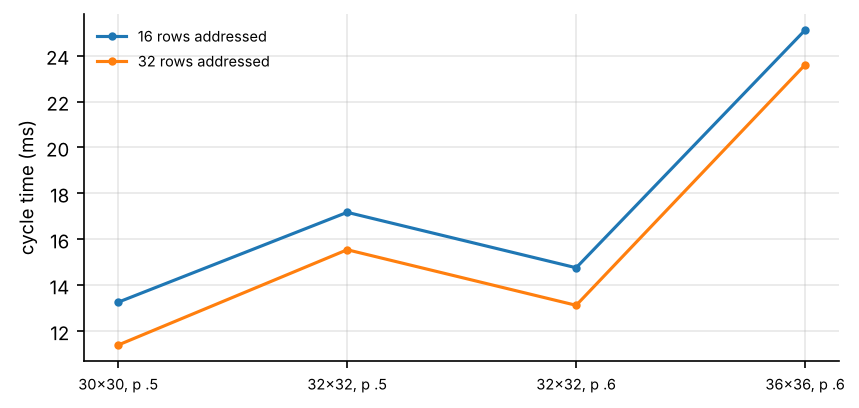
\includegraphics[width=0.8\linewidth]{m20_rearrange.png}
\caption{Mean cycle time of one rearrangement cycle (greedy scheduler, 40 random loadings of a $50\times45$ array at 4~\textmu m pitch) for four target blocks and loading probabilities $p$, with one 16-chip stack (16 rows addressed) and two combined stacks (32 rows addressed). Timing: 100~\textmu s ramps, 400~\textmu s lane steps, minimum-jerk $x$ moves of 400~\textmu s per 40~\textmu m scaled as $\sqrt{d}$ (at least 200~\textmu s), 0.3~ms scanner settling per pass. The second stack saves one compaction pass in each case.}
\label{fig:rearrange-cycle}
\end{figure}

The cycle time depends mainly on the fixed costs of a pass (Table~\ref{tab:rearrange-timing}). The low-heating steps of Sec.~\ref{sec:transport-timing} raise it from 17.2 to 18.8~ms. Shortening the lane steps to 100~\textmu s gives 12.5~ms, and making everything fast gives 8.2~ms, while slower scanner settling (1~ms) gives 22.7~ms. Because vacuum loss grows with cycle time, the all-fast setting halves it (0.28 defects at 30~s). It costs heating: about 10~\textmu K per move at a moving depth of 0.3~mK, or 1.2~\textmu K at 0.5~mK. Thus two regimes remain: slow and cold at 0.3~mK, with low power, or fast at 0.5~mK. With the slow steps (0.29~\textmu K per move, lateral handoff plus $x$ move) the block gains 0.33~\textmu K on average and 0.58~\textmu K for an atom moved twice; with fast steps at 0.5~mK the corresponding figures are 1.36 and 2.42~\textmu K.

\begin{table}[htbp]\centering\small
\caption{Sensitivity of the cycle time to the step timing ($32\times32$ block, 50\% loading, one stack, mean of 40 loadings; simulated).}
\label{tab:rearrange-timing}
\begin{tabular}{ll}
\toprule
timing & cycle time \\
\midrule
base (ramps 100~\textmu s, lane steps 400~\textmu s) & 17.2~ms \\
low heating (ramps 200~\textmu s, lane steps 400~\textmu s) & 18.8~ms \\
fast lane steps (100~\textmu s) & 12.5~ms \\
all fast (ramps 50~\textmu s, lane steps 100~\textmu s, $x$ 200~\textmu s per 40~\textmu m) & 8.2~ms \\
scanner settling 1~ms instead of 0.3~ms & 22.7~ms \\
\bottomrule
\end{tabular}
\end{table}

\subsection{Pass selection and the pass floor}\label{sec:rearrange-modes}

We compared three ways of selecting the balancing passes on 40 loadings ($32\times32$, 50\%, one stack): greedy (most atoms per pass), rate (most atoms per unit pass time) and lookahead (best two-pass sequence among the 8 best first passes). They need 8.05, 8.05 and 7.98 passes in all, with mean cycle times of 17.8, 17.6 and 17.6~ms (maxima 23.1, 22.8 and 22.9~ms). The three modes agree to within 1\%. This is because the balancing stage has a geometric floor of about four passes. In one pass the 16-row window can hold at most 9 non-target rows above or below the 32-row target band, so it can feed at most 9 target rows; feeding all 32 therefore takes at least four passes, plus two compaction passes. The greedy schedule (5.8 + 2) is within about 30\% of that floor. Further gains would come from shorter passes, not from fewer.

\subsection{Stochastic losses and defects}\label{sec:rearrange-loss}

The scheduler fills every loading; defects come from losses. The loss per move is not computed by the transport simulations, which bound it below about $10^{-3}$ (0 of 3,000 atoms lost); we take $10^{-3}$ and $10^{-4}$, the latter an assumption. Vacuum lifetimes of 30 and 300~s are also assumed. At $10^{-3}$ per move the $32\times32$ cycle leaves 1.15 defects on average and at $10^{-4}$ 0.12; vacuum loss during the 17~ms adds 0.59 defects at 30~s and 0.06 at 300~s (Table~\ref{tab:rearrange-cycle}). The probability that the block is defect-free after one cycle is 0.84 at $10^{-4}$ per move and 300~s. Reaching 0.99 in one cycle would need about $5\times10^{-6}$ loss per move and a vacuum lifetime above about one hour. A repair round after imaging is the realistic route.

\subsection{Image-and-repair rounds}\label{sec:rearrange-repair}

After the cycle, the array is imaged (10~ms, our choice) and each hole in the block is filled directly by one reservoir atom, moved through the lanes from the nearest rows under the same pass rules. This takes 0.1 to 1.3 repair passes, so a round lasts 10 to 13~ms. The repair works, but it cannot go below a floor set by the image itself: atoms lost because of the image are not seen by it, and every atom is exposed to vacuum loss for the duration of the round. The expected number of defects after a round is
\begin{equation}
  n_\mathrm{d} \approx N\left(\epsilon_\mathrm{img} + \frac{t_\mathrm{round}}{\tau}\right) + p_\mathrm{move}\, n_\mathrm{rep}.
  \label{eq:rearrange-floor}
\end{equation}
Here, $N=1024$ is the number of sites in the block, $\epsilon_\mathrm{img}$ the loss per image, $t_\mathrm{round}$ the duration of the round, $\tau$ the vacuum lifetime, $p_\mathrm{move}$ the loss per move and $n_\mathrm{rep}$ the number of repair moves. For $\epsilon_\mathrm{img}=10^{-4}$ and $\tau=300$~s this gives about 0.14 defects, and a second round does not lower it (Table~\ref{tab:rearrange-repair}).

\begin{table}[htbp]\centering\small
\caption{Probability of a defect-free $32\times32$ block after the cycle and after one and two image-and-repair rounds, and expected defects after one round (simulated, 40 loadings $\times$ 25 loss draws per row; all loss rates and lifetimes assumed).}
\label{tab:rearrange-repair}
\setlength{\tabcolsep}{3.5pt}
\begin{tabular}{lllll}
\toprule
loss per move & lifetime & loss per image & P(defect-free): cycle / 1 / 2 rounds & defects after 1 repair \\
\midrule
$10^{-3}$ & 300~s & $10^{-4}$ & 0.27 / 0.87 / 0.87 & 0.14 \\
$10^{-4}$ & 300~s & $10^{-4}$ & 0.84 / 0.87 / 0.87 & 0.14 \\
$10^{-3}$ & 300~s & $10^{-3}$ & 0.27 / 0.35 / 0.33 & 1.04 \\
$10^{-4}$ & 300~s & $10^{-3}$ & 0.84 / 0.35 / 0.33 & 1.03 \\
$10^{-3}$ & 30~s & $10^{-4}$ & 0.14 / 0.59 / 0.62 & 0.53 \\
$10^{-4}$ & 30~s & $10^{-4}$ & 0.48 / 0.62 / 0.63 & 0.48 \\
\bottomrule
\end{tabular}
\end{table}

As can be seen from Table~\ref{tab:rearrange-repair}, a repair round brings poor transport ($10^{-3}$ per move) up to the same 0.87 as good transport, provided the image is gentle. Once the loss per move is about $10^{-4}$ or less, the probability of a defect-free block is set by the imaging loss and the vacuum lifetime, not by the transport. With good transport and an imaging loss of $10^{-3}$, a repair round makes things worse: 0.84 becomes 0.35, because the image costs about one atom of the block. Imaging should then be skipped, or used only to post-select. For a 99\% defect-free block each term of Eq.~\eqref{eq:rearrange-floor} must be near $10^{-5}$: the loss per move, the loss per image, and $t_\mathrm{round}/\tau$. The continuous version of this balance, with periodic imaging and refilling of much larger arrays, is the subject of Sec.~\ref{sec:megascale}.

\subsection{Limits}\label{sec:rearrange-limits}

The scheduler is greedy and not optimised across stack positions. The loss per move is bounded by the transport simulations but not computed, and the values used here, like the imaging time, imaging loss and vacuum lifetimes, are assumptions. Detection is taken as perfect apart from the imaging-induced loss, with no false positives or negatives. The repair model moves one reservoir atom per hole. Photon scattering by the trapping light (estimated at a few photons per second at 0.3 to 0.5~mK) is not included, and neither is the possibility that an atom heated by its moves is lost during later moves. The heating per move comes from the one-dimensional quantum check and the three-dimensional classical runs of Sec.~\ref{sec:transport-timing}, with the axial focus offset held to $\pm0.5$~\textmu m (Sec.~\ref{sec:transport-tol}).

\section{Arrays of $10^4$ to $10^6$ sites}\label{sec:megascale}

We ask what limits an array of $10^4$, $10^5$ or $10^6$ sites at 3 to 4~\textmu m pitch, in the order in which the limits appear, and what the transport hardware of the previous chapters must look like to assemble such an array and keep it filled. The record is \texttt{docs/\allowbreak megascale.md} (Secs.~1 to 10); the code is \texttt{scripts/m22\_megascale.py} (budget, tiling), \texttt{picsim/megasort.py} with \texttt{scripts/m23\_steady.py} (assembly and steady state), \texttt{scripts/m24\_tiling\_wave.py} and \texttt{scripts/m25\_imaging.py}.

The short answer is as follows. At 4~\textmu m pitch the transport side scales to $10^6$ sites. An engine block of 32 rows $\times$ 4 engines (128 engines) assembles $10^6$ sites from 85\% loading to $10^{-3}$ defects in 1.0 to 1.1~s with fast handoff steps, and then holds the array at a time-averaged defect fraction of $1.8\times10^{-4}$ ($2.4\times10^{-4}$ sampled at the image). Three walls come first: (i) the corrected field of the objective, (ii) the static trapping power, which is the first wall at $10^6$ sites, and (iii) the loss rates (vacuum lifetime and loss per image), which set the steady-state floor at every array size. At $10^6$ sites the transport adds a fourth constraint, the latency of a block that must sweep 252 positions to reach a hole; it is removed by fast steps, a larger block, or a slower imaging cadence. Table~\ref{tab:mega-overview} collects the scale-dependent numbers.

\begin{table}[htbp]\centering\small
\caption{Scale of the problem (derived, \texttt{results/\allowbreak m22\_budget.json}). Field radius $L/\sqrt{2}$ for a square of side $L$; resolution cell 1.06~\textmu m at NA 0.5; static power at 4.5~mW per site per mK, 85\% loading including the reservoir; block positions for the 32~$\times$~4 block at 4~\textmu m pitch; refills for $\tau=3000$~s and $\epsilon_\mathrm{img}=10^{-4}$ at 10~Hz imaging.}
\label{tab:mega-overview}
\begin{tabular}{lccc}
\toprule
 & $10^4$ sites & $10^5$ sites & $10^6$ sites \\
\midrule
side at 4 / 3~\textmu m pitch & 0.40 / 0.30~mm & 1.26 / 0.95~mm & 4.0 / 3.0~mm \\
single objective: field radius (4~\textmu m) & 0.28~mm & 0.89~mm & 2.8~mm \\
resolution cells per side (4~\textmu m) & 372 & 1,187 & 3,754 \\
zones of $\pm250$~\textmu m (objectives) & 2 & 13 & 127 \\
static power at the atoms, 0.1 / 1~mK & 5.3 / 53~W & 53 / 530~W & 0.53 / 5.3~kW \\
32~$\times$~4 block: positions & 10 & 28 & 252 \\
refills needed per second & 13 & 134 & 1,335 \\
\bottomrule
\end{tabular}
\end{table}

\subsection{The walls in order}\label{sec:megascale-walls}

\paragraph{Field and space-bandwidth.} A square array of side $L$ needs a corrected field of radius $L/\sqrt{2}$. At 4~\textmu m pitch that is 372, 1,187 and 3,754 resolution cells per side for $10^4$, $10^5$ and $10^6$ sites; the last corresponds to a space-bandwidth product of about $1.4\times10^7$. The $\pm100$~\textmu m field of the proposal~\cite{proposal} covers none of these. $10^4$ sites need $\pm0.28$~mm. $10^5$ sites need $\pm0.9$~mm, which is within the range of refractive NA 0.5 objectives (recalled, to be verified). $10^6$ sites need a lithography-class field of $\pm2.8$~mm at NA 0.5. Zones, i.e.\ independent arrays each with its own objective, static array and engine block, avoid the large field. A $\pm250$~\textmu m zone holds 7,700 sites at 4~\textmu m and assembles like the $10^4$ case. However, each zone needs its own objective, about 25 to 30~mm across at a 15~mm working distance, so the 127 zones needed for $10^6$ sites are impractical. Zones therefore suit $10^4$ (2 zones) to $10^5$ sites (13 zones); at $10^6$ a single large-field objective, or a few large zones, cannot be avoided.

\paragraph{Static trapping power.} From the trap depth with $\alpha(1075~\mathrm{nm})=1120$~au and a 0.85~\textmu m waist, a tweezer needs 4.5~mW per site per mK at the atoms. The reservoir sites count as well. The budget of Table~\ref{tab:mega-overview} uses the minimum reservoir fraction $1-f$, i.e.\ 50\% of all sites at 50\% loading and 15\% at 85\%; the simulated 3:1 layout at 85\% uses 25\%, which adds 13\% to these powers. At the 0.1~mK hold of the transport model (Sec.~\ref{sec:transport}), $10^6$ sites take 0.5 to 0.9~kW at the atoms (85\% to 50\% loading), and 5 to 9~kW at a 1~mK loading or imaging depth. With an assumed delivery efficiency of 30\%, the laser must supply 1.8 to 3~kW at the hold and 18 to 30~kW at 1~mK. This is the first wall at $10^6$ sites.

An optical lattice is the obvious alternative for the static potential, as in the continuously operated lattice array of Gyger et al.~\cite{gyger2024} (known to us from a search summary only). Table~\ref{tab:mega-static} compares the two (derived, \texttt{results/\allowbreak m22\_lattice.json}). The lattice uses two orthogonal retro-reflected beams (incoherent sum, peak $8I$ per beam; coherent four-beam sum, $16I$), held within $-20\%$ of the peak over the array. A tweezer puts its power into about $\pi w_0^2/2=1.1$~\textmu m$^2$ per site. A Gaussian lattice beam that keeps the corners within 20\% spreads it over about $15a^2/G=31$~\textmu m$^2$. Hence a free-space lattice loses to tweezers by about 25 with Gaussian beams and by 2 to 4 with flat-top beams. Only an enhancement cavity with a buildup near 100 wins, by a factor of about 4, and that cavity would need a waist near 10~mm for $10^6$ sites. Two levers do more than the choice of potential: the depth (a factor of 10 between 1 and 0.1~mK), and the delivery efficiency, which for the simpler lattice optics could gain up to about 2.7 (0.8 instead of 0.3). For $10^6$ sites the static potential thus needs about 2~kW of laser power at the hold depth with tweezers, or about 0.5~kW with a buildup-100 cavity lattice, and loading and imaging must happen at a lower depth or in a smaller zone.

\begin{table}[htbp]\centering\small
\caption{Laser power for the static potential at 30\% delivery (assumed), for $N$ sites plus a 25\% reservoir at 4~$\times$~4~\textmu m, at depths of 0.1 / 1~mK (derived, \texttt{results/\allowbreak m22\_lattice.json}). Lattices: two orthogonal retro-reflected beams held within $-20\%$ of the peak; cavity buildup is a choice.}
\label{tab:mega-static}
\begin{tabular}{lccc}
\toprule
static potential & $10^4$ sites & $10^5$ sites & $10^6$ sites \\
\midrule
tweezer array ($w_0=0.85$~\textmu m) & 20 / 200~W & 0.2 / 2.0~kW & 2.0 / 20~kW \\
free-space lattice, Gaussian beams & 0.5 / 5.0~kW & 5 / 50~kW & 50 / 500~kW \\
free-space lattice, flat-top, incoherent & 85~W / 0.85~kW & 0.85 / 8.5~kW & 8.5 / 85~kW \\
free-space lattice, flat-top, coherent & 42~W / 0.42~kW & 0.42 / 4.2~kW & 4.2 / 42~kW \\
cavity lattice, Gaussian, buildup 10 & 50~W / 0.5~kW & 0.5 / 5~kW & 5 / 50~kW \\
cavity lattice, Gaussian, buildup 100 & 5 / 50~W & 0.05 / 0.5~kW & 0.5 / 5~kW \\
\bottomrule
\end{tabular}
\end{table}

\paragraph{Engines, blocks and tiling along $x$.} One engine (192 ports, 383 fast actuators, Sec.~\ref{sec:engine}) serves a 180~\textmu m row segment, i.e.\ 45 to 46 sites at 4~\textmu m and 60 to 61 at 3~\textmu m. Engines can be tiled in two directions. Along $y$, chips are stacked, one chip per row with its own collimator (Sec.~\ref{sec:rows}). Along $x$, several engines share one chip edge: each gets its own $x$ lenslet, and a common Fourier lens overlaps all of them in the pupil and maps their offsets to adjacent atom segments. The ABCD check (\texttt{m22\_tiling}) gives a magnification of $-60.1$ for every engine and all chief rays at the pupil centre. The question is how close the engines can sit. A first-order argument gave a pessimistic answer: with 1.5~\textmu m emitter pitch, each engine's first grating lobe lands 204~\textmu m from its spot at the atoms, inside the neighbouring segment, so a shared slit plane would need opaque gaps as wide as the slit zones, and hence an engine pitch $P_e\geq4.4$~mm (four engines per 18~mm edge).

The wave-optics check (\texttt{results/\allowbreak m24\_tiling\_wave.json}) supersedes this. We propagate the emitter near field of one D1 engine, forming a tweezer at $x_a=0$, 60 and 90~\textmu m (up to the segment edge), over $f_1=3.12$~mm to its lenslet (clear aperture equal to fill $\times P_e$), apply an ideal lens phase, propagate over $f_1$ to the shared slit plane $\Sigma$, and measure the intensity in the neighbouring engine's slit zone. Here, $\Sigma$ is conjugate to the atoms, so this intensity is the ghost that a neighbouring segment sees. We keep only directions inside the pupil acceptance $A/(2f_1)$, because steeper light misses the objective, and an exact ray trace through the neighbouring lenslets checks the same question geometrically. Table~\ref{tab:mega-tiling} and Fig.~\ref{fig:mega-tiling} give the result. The first-order lobes are not the limit: the lenslet aperture and the pupil acceptance remove them, and no accepted ray reaches another slit zone at any pitch scanned. What sets the pitch is the lenslet aperture needed to pass the engine's own slit zone, $2f_1\tan(\arcsin s_\mathrm{cut})=2.37$~mm. Below 2.6~mm the lenslet clips the engine's own beam and its diffraction tail enters the neighbouring zone. At $P_e=3.0$~mm the accepted ghost is below $2\times10^{-7}$ of a tweezer peak, under the coherent criterion of $10^{-6}$ (\texttt{docs/\allowbreak row\_coherence.md}). Hence six engines fit on an 18~mm chip edge instead of four. Two scanner positions per row are still needed: the segment pitch at the atoms, $P_e f_\mathrm{obj}/f_c=0.092\,P_e=277$~\textmu m at $P_e=3.0$~mm ($f_c=188$~mm, $f_\mathrm{obj}=17.3$~mm), exceeds the 180~\textmu m segment, so one block position addresses every other segment. The model is 1D ($x$ only) with an ideal thin lens and no surface scatter; baffles between the lenslet channels remain the defence against scattered light, which it does not include.

\begin{table}[htbp]\centering\small
\caption{Ghost of one engine in its neighbour's slit zone versus engine pitch $P_e$ (simulated, 1D, \texttt{results/\allowbreak m24\_tiling\_wave.json}). Worst case over $x_a=0$, 60, 90~\textmu m at lenslet fill 1 (the segment-edge tweezer, except at 3.5~mm where $x_a=60$~\textmu m is marginally worse). ``Accepted'' keeps only directions inside the pupil acceptance. A fill of 0.8 at 4.43~mm raises the accepted ghost to $2\times10^{-9}$. No accepted ray through a neighbouring lenslet reaches another slit zone at any pitch.}
\label{tab:mega-tiling}
\begin{tabular}{lccc}
\toprule
 & \multicolumn{2}{c}{ghost peak / tweezer peak} & ghost power / \\
$P_e$ & accepted & raw & own slit power \\
\midrule
8.0~mm & $4.5\times10^{-13}$ & $1.7\times10^{-9}$ & $2.6\times10^{-13}$ \\
4.43~mm & $3.6\times10^{-10}$ & $2.5\times10^{-7}$ & $1.4\times10^{-10}$ \\
3.5~mm & $1.7\times10^{-8}$ & $3.1\times10^{-6}$ & $1.0\times10^{-8}$ \\
3.0~mm & $1.7\times10^{-7}$ & $7.7\times10^{-6}$ & $6.3\times10^{-8}$ \\
2.6~mm & $1.6\times10^{-6}$ & $1.3\times10^{-5}$ & $7.5\times10^{-7}$ \\
2.4~mm & $6.7\times10^{-5}$ & $5.6\times10^{-5}$ & $7.2\times10^{-5}$ \\
\bottomrule
\end{tabular}
\end{table}

\begin{figure}[htbp]\centering
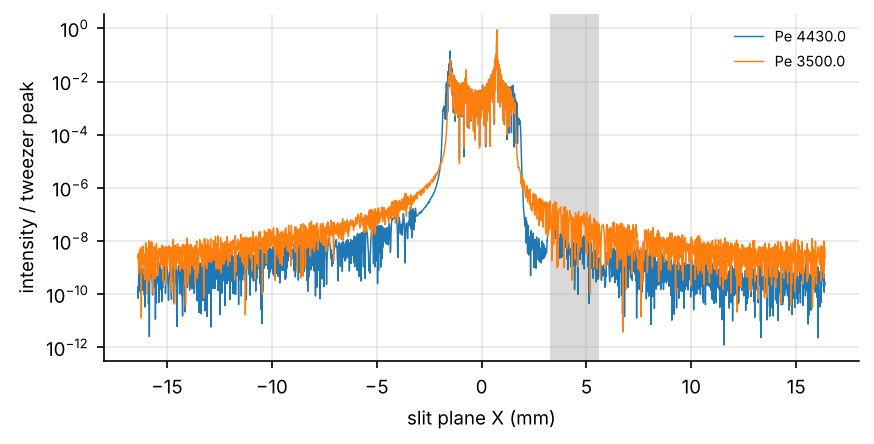
\includegraphics[width=0.8\linewidth]{m24_tiling_wave.png}
\caption{Intensity at the shared slit plane $\Sigma$, relative to the tweezer peak, for one D1 engine forming a tweezer at the segment edge ($x_a=90$~\textmu m), lenslet fill 1, engine pitch 4.43~mm (blue) and 3.5~mm (orange). 1D angular-spectrum propagation of the emitter near field over $f_1=3.12$~mm, ideal lens phase on the lenslet aperture, and propagation over $f_1$ (0.25~\textmu m grid). The grey band is the neighbouring engine's slit zone at 4.43~mm pitch, $|X-P_e|<f_1 s_\mathrm{cut}$. The curves show the raw intensity, before the pupil-acceptance filter applied in Table~\ref{tab:mega-tiling}.}
\label{fig:mega-tiling}
\end{figure}

A block of 32 rows (two 16-chip stacks, combined by polarisation or by the comb of Sec.~\ref{sec:combine}) $\times$ 4 engines per row has 128 engines and 49,024 fast actuators. It holds 5,888 simultaneous tweezers, which need 85~W at 0.3~mK if all are lit; that happens at most during assembly, since in steady state only the few refilling tweezers are lit. A single 16-chip stack (a 16~$\times$~1 block) is too small for $10^6$ sites: it never finishes assembling.

\paragraph{Pitch.} At 3~\textmu m pitch in both directions the transport lane passes 1.5~\textmu m from waiting atoms, and the moving tweezer pulls most of them out, so such a lattice would need empty corridor rows. The anisotropic lattice avoids this (Sec.~\ref{sec:transport}): with 3~\textmu m along the rows and rows 4~\textmu m apart, the lane stays 2~\textmu m from the rows and the lattice transports as cleanly as 4~$\times$~4~\textmu m. It has 33\% more sites per area (0.063 against 0.047 computation sites per \textmu m$^2$ with a 3:1 reservoir layout). Below, ``3~\textmu m'' means this 3~$\times$~4~\textmu m lattice.

\subsection{Assembly and steady-state refilling}\label{sec:megascale-steady}

The simulation (\texttt{picsim/megasort.py}) represents the array as computation rows interleaved with reservoir rows (1:2 at 50\% loading, 3:1 at 85\%). The array is imaged every $T_\mathrm{img}=0.1$~s for $t_\mathrm{img}=10$~ms, with a loss $\epsilon_\mathrm{img}=10^{-4}$ per image and $10^{-4}$ per move; the reservoir is refreshed every 1~s from an external supply. The engine block visits, round-robin, the tiles with known holes, and each visit runs up to four repair passes (a common row shift, an order-preserving $x$ pass, and one move per refill). Two step timings come from the rearrangement chapter (Sec.~\ref{sec:rearrange}): slow (200~\textmu s ramps, 400~\textmu s lane steps, 0.2 to 0.3~\textmu K per move) and fast (50~\textmu s ramps, 100~\textmu s lane steps, 200~\textmu s per 40~\textmu m, about 1 to 10~\textmu K per move). Table~\ref{tab:mega-assembly} and Fig.~\ref{fig:mega-steady} summarise the runs at 4~\textmu m pitch. Their steady-state values are sampled just after an image; Sec.~\ref{sec:megascale-defects} explains why the time average is lower.

\begin{table}[htbp]\centering\small
\caption{Assembly and steady state at 4~\textmu m pitch (simulated, \texttt{results/\allowbreak m23\_steady.json}). Time from a random loading to $10^{-2}$ and $10^{-3}$ defects (n.r.: not reached in 20~s), and the steady-state defect fraction sampled just after each image, in units of $10^{-4}$, for $\tau=3000$ / 300~s. Slow and fast step timings as in the text. At $10^6$ sites with $\tau=300$~s, slow steps do not reach $10^{-3}$.}
\label{tab:mega-assembly}
\begin{tabular}{llllccc}
\toprule
sites & loading & block & timing & to $10^{-2}$ & to $10^{-3}$ & steady state, $\tau$ 3000 / 300~s \\
\midrule
$10^4$ & 50\% & 16$\times$1 & slow & 0.34~s & 0.34~s & 2.7 / 5.6 \\
$10^4$ & 50\% & 32$\times$4 & slow & 0.12~s & 0.12~s & 2.6 / 5.6 \\
$10^4$ & 85\% & 32$\times$4 & slow & 0.12~s & 0.12~s & 1.8 / 5.7 \\
$10^5$ & 50\% & 16$\times$1 & slow & 1.8~s & 1.8--2.8~s & 2.3 / 6.0 \\
$10^5$ & 50\% & 32$\times$4 & slow & 0.46~s & 0.46~s & 2.5 / 6.1 \\
$10^5$ & 85\% & 32$\times$4 & slow & 0.24~s & 0.24~s & 2.5 / 5.8 \\
$10^5$ & 85\% & 32$\times$4 & fast & 0.12~s & 0.12~s & 2.5 ($\tau$ 3000~s) \\
$10^6$ & 50\% & 32$\times$4 & slow & 2.2~s & 2.8~s ($\tau$ 3000~s) & 8.6 / 32 \\
$10^6$ & 85\% & 32$\times$4 & slow & 1.9~s & 3.1~s ($\tau$ 3000~s) & 9.3 / 38 \\
$10^6$ & 85\% & 32$\times$4 & fast & 0.79~s & 1.1~s & 2.4 ($\tau$ 3000~s) \\
$10^6$ & 50\% / 85\% & 16$\times$1 & slow & 14~s ($\tau$ 3000~s) & n.r. & 70 to 290 \\
\bottomrule
\end{tabular}
\end{table}

\begin{figure}[htbp]\centering
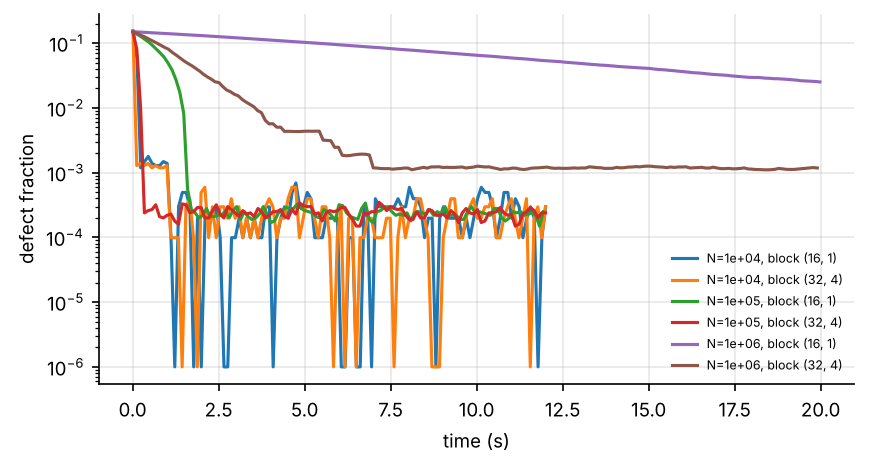
\includegraphics[width=0.8\linewidth]{m23_steady.png}
\caption{Defect fraction sampled just after each image versus time, from a random 85\% loading (3:1 computation to reservoir rows) at 4~\textmu m pitch, slow steps, $\tau=3000$~s, $\epsilon_\mathrm{img}=10^{-4}$ per image and per move, imaging every 0.1~s, for blocks of 16~$\times$~1 and 32~$\times$~4 engines and $10^4$ to $10^6$ sites (\texttt{scripts/m23\_steady.py}). Values of zero are drawn at $10^{-6}$. With slow steps, $10^6$ sites with the 32~$\times$~4 block settle at the latency-limited $9\times10^{-4}$, and the 16~$\times$~1 block does not reach $10^{-3}$. Fast steps (not shown) restore the loss-limited floor.}
\label{fig:mega-steady}
\end{figure}

Three findings follow. (i) Up to $10^5$ sites the floor is set by the losses, and it is nearly the same for every block and timing (1.7 to $2.7\times10^{-4}$ at image for $\tau=3000$~s, the spread being run-to-run noise). (ii) At $10^6$ sites latency matters: with slow steps a sweep of 252 block positions takes longer than the imaging period, new holes wait several sweeps, and the floor rises about four-fold. Fast steps restore the loss-limited floor. (iii) Each refill is a single move from a nearby reservoir row into the hole, so heating does not accumulate on any atom. In steady state at $10^6$ sites the reservoir is consumed at about 1,300 atoms per second ($\tau=3000$~s). Chiu et al.~\cite{chiu2025} (abstract read) report 30,000 initialized qubits per second from lattice conveyor belts, maintaining more than 3,000 atoms for over 2 hours; that rate would cover our demand with a margin of 20. For comparison with our loss parameters, Manetsch et al.~\cite{manetsch2024} (abstract read) report a 23~min lifetime in a room-temperature apparatus and 99.98952\% imaging survival ($\epsilon_\mathrm{img}=1.05\times10^{-4}$) for a 6,100-atom Cs tweezer array, i.e.\ close to our nominal $\epsilon_\mathrm{img}$ and a lifetime between our 300~s and 3000~s cases.

\subsection{Three defect fractions}\label{sec:megascale-defects}

The values of Table~\ref{tab:mega-assembly} are sampled just after each image. That value counts imaging losses twice. An image removes a fraction $\epsilon_\mathrm{img}$ of the atoms after detecting them, so these holes stay unseen for a full period, and at the next image they are still present when the new losses are added. The simulator therefore also records the value just before each image and the time average. The time average is a trapezoid sum over visit, image and idle intervals; it is exact in expectation for the vacuum losses, which are uniform in time, while each visit's fills are booked at its start, which biases the average low by at most one visit time (1 to 2~ms against $T_\mathrm{img}=100$~ms). The time average is what a computation started at a random moment sees. With fast steps at $10^6$ sites the three values are $2.4\times10^{-4}$ (at image), $1.4\times10^{-4}$ (before image) and $1.8\times10^{-4}$ (time average). The at-image value is close to $2\epsilon_\mathrm{img}+(T_\mathrm{img}+t_\mathrm{img})/\tau=2.4\times10^{-4}$, and the time average is close to $\epsilon_\mathrm{img}+(T_\mathrm{img}+t_\mathrm{img})/(2\tau)=1.2\times10^{-4}$ plus the repair latency. Thus the time average is about 25\% below the at-image figures quoted in Table~\ref{tab:mega-assembly}, and an earlier rule $\rho\approx(1.5\text{ to }1.8)(\epsilon_\mathrm{img}+T_\mathrm{img}/\tau)$, fitted to at-image values over a narrower range, is replaced by the fits of Sec.~\ref{sec:megascale-imaging}.

\subsection{Remedies at \texorpdfstring{$10^6$}{10\textasciicircum 6} sites}\label{sec:megascale-remedies}

At $10^6$ sites the choice is between a larger block and faster, hotter steps. We scanned blocks of 128 to 256 engines and three step timings with heating per move of 10~\textmu K (fast), 2~\textmu K (intermediate) and 0.3~\textmu K (slow), at 85\% loading, $\tau=3000$~s, $\epsilon_\mathrm{img}=10^{-4}$, $T_\mathrm{img}=100$~ms and rows 4~\textmu m apart (\texttt{results/\allowbreak m23\_remedy.json}, one seed per case). The intermediate timing (100~\textmu s ramps, 200~\textmu s lane steps) transports cleanly on the 3~$\times$~4~\textmu m lattice at 1 to 3~\textmu K per move with no bystander lost or displaced (\texttt{results/\allowbreak m18\_midlane.json}, 3,000 atoms per case; Sec.~\ref{sec:transport}); we use 2~\textmu K per move. Table~\ref{tab:mega-remedy} gives the results.

\begin{table}[htbp]\centering\small
\caption{Remedies at $10^6$ sites (simulated, \texttt{results/\allowbreak m23\_remedy.json}; 85\% loading, $\tau=3000$~s, $\epsilon_\mathrm{img}=10^{-4}$, $T_\mathrm{img}=100$~ms, rows 4~\textmu m apart). Each cell: defect fraction at image / time average over the last 3~s of a 20~s run, in units of $10^{-4}$; then the time from the first image to $10^{-3}$ at image. Heating per move 10 / 2 / 0.3~\textmu K; loss per move $4\times10^{-3}$ for fast steps (from the 3D transport model with 50~\textmu s ramps) and $10^{-4}$ otherwise.}
\label{tab:mega-remedy}
\begin{tabular}{llccc}
\toprule
block (engines) & pitch along rows & fast & intermediate & slow \\
\midrule
32$\times$4 (128) & 4~\textmu m & 2.5 / 2.0; 1.01~s & 4.6 / 4.1; 1.25~s & 9.1 / 8.6; 3.56~s \\
32$\times$8 (256) & 4~\textmu m & 2.4 / 1.8; 0.68~s & 3.4 / 2.9; 0.92~s & 6.4 / 5.9; 1.39~s \\
48$\times$4 (192) & 4~\textmu m & 2.5 / 1.9; 0.68~s & 3.6 / 3.1; 0.92~s & 6.7 / 6.2; 1.40~s \\
64$\times$4 (256) & 4~\textmu m & 2.4 / 1.8; 0.45~s & 3.2 / 2.7; 0.69~s & 5.5 / 4.9; 1.05~s \\
32$\times$4 (128) & 3~\textmu m & 2.4 / 1.9; 0.79~s & 4.1 / 3.6; 1.14~s & 7.9 / 7.4; 2.31~s \\
32$\times$8 (256) & 3~\textmu m & 2.4 / 1.8; 0.56~s & 3.0 / 2.5; 0.80~s & 5.0 / 4.5; 1.17~s \\
48$\times$4 (192) & 3~\textmu m & 2.4 / 1.8; 0.56~s & 3.5 / 2.9; 0.80~s & 5.9 / 5.3; 1.17~s \\
64$\times$4 (256) & 3~\textmu m & 2.4 / 1.8; 0.46~s & 2.9 / 2.4; 0.58~s & 4.9 / 4.4; 0.94~s \\
\bottomrule
\end{tabular}
\end{table}

Four results follow. First, fast steps reach the loss floor with any block from 128 engines; more engines only shorten assembly (1.01 to 0.45~s at 4~\textmu m). The 3~$\times$~4~\textmu m lattice holds $2.4\times10^{-4}$ at image with the 32~$\times$~4 block, as 4~$\times$~4~\textmu m does. An earlier value of $8.1\times10^{-4}$ for this case was an artefact of the block placement: the last row of block positions ended short of the array edge, so the holes in the rows below it had no reservoir row in any block that reached them (563 of 716 remaining holes sat there); the last block now sits flush with the edge. Second, intermediate steps come within a factor of 1.3 to 1.6 of the floor with 256 engines (time average $2.4$ to $2.9\times10^{-4}$), and within a factor of 2 to 2.3 with 128. Third, slow steps reach $10^{-3}$ within 1 to 3.6~s with every block, but hold $4.4$ to $8.6\times10^{-4}$, a factor of 2.4 to 4.8 above the floor. Fourth, the 3~\textmu m rows do slightly better than 4~\textmu m rows with the slower timings. We attribute this to fewer block positions per sweep (a 180~\textmu m segment holds 61 sites at 3~\textmu m against 46 at 4~\textmu m, so the 32~$\times$~4 block needs 222 positions instead of 252), but we did not isolate this cause.

The heating cost is set per refilled atom, not per atom in the array. Every atom moves at most once, because refills come straight from a reservoir row; with the 32~$\times$~4 block at $10^6$ sites 17\% of the atoms are moved, and the heating is 0.05~\textmu K mean and 0.3~\textmu K maximum with slow steps, against 1.7 and 10~\textmu K with fast steps (\texttt{results/\allowbreak m23\_mixed.json}). An adaptive schedule (fast until $10^{-2}$, then slow) brings back the latency-limited floor of $9\times10^{-4}$ at image: the refill load at $10^6$ sites is too high for slow steps in steady state. Up to $10^5$ sites, slow and cold steps reach the loss-limited floor.

The block shape is a hardware choice. A 32-row block is two 16-chip stacks; 48 or 64 rows need three or four stacks and a combining method beyond polarisation, which Sec.~\ref{sec:combine} provides (a slotted comb mirror, with a polarising beam splitter for 64 rows). A 32~$\times$~8 block needs eight engines per chip edge, i.e.\ a 24~mm edge at the 3.0~mm engine pitch; at 2.6~mm (21~mm edge) the accepted ghost rises to $1.6\times10^{-6}$, just above the $10^{-6}$ criterion. The 64~$\times$~4 block has the same 256 engines on 12~mm chip edges and does slightly better with intermediate steps (time average $2.7\times10^{-4}$ on 4~$\times$~4 and $2.4\times10^{-4}$ on 3~$\times$~4~\textmu m), and Sec.~\ref{sec:combine} shows that it can be built. At the same time, Sec.~\ref{sec:combine} finds that the refractive collimator serves only half of each 180~\textmu m segment, which doubles the number of engines per row at fixed coverage; the block counts above assume full segments.

\subsection{Imaging cadence and the hole lifetime}\label{sec:megascale-imaging}

Since the floor follows the losses, we scanned the imaging parameters at $10^5$ sites (4~$\times$~4~\textmu m, 85\% loading, 32~$\times$~4 block, intermediate steps, $t_\mathrm{img}=10$~ms, runs of 8~s or longer averaged over the second half, one seed per case; \texttt{results/\allowbreak m25\_imaging.json}): $T_\mathrm{img}=0.03$, 0.1, 0.3 and 1~s, $\epsilon_\mathrm{img}=10^{-5}$, $10^{-4}$ and $10^{-3}$, and $\tau=300$, 3000 and 30000~s, with $t_\mathrm{img}=3$ and 20~ms added, and three points per timing at $10^6$ sites. The at-image values fit
\begin{equation}
\rho_\mathrm{image}=2.24\,\epsilon_\mathrm{img}+0.98\,\frac{T_\mathrm{img}+t_\mathrm{img}}{\tau}
\end{equation}
with a median error of 10\% (worst 40\%), close to the $2\epsilon_\mathrm{img}+(T_\mathrm{img}+t_\mathrm{img})/\tau$ expected from the double counting (Fig.~\ref{fig:mega-imaging}). Table~\ref{tab:mega-imaging} gives selected time averages.

\begin{table}[htbp]\centering\small
\caption{Time-averaged defect fraction at $10^5$ sites versus imaging period (simulated, \texttt{results/\allowbreak m25\_imaging.json}; 4~$\times$~4~\textmu m, 85\% loading, 32~$\times$~4 block, intermediate steps, $t_\mathrm{img}=10$~ms).}
\label{tab:mega-imaging}
\begin{tabular}{lcccc}
\toprule
$\epsilon_\mathrm{img}$, $\tau$ & $T_\mathrm{img}=0.03$~s & 0.1~s & 0.3~s & 1~s \\
\midrule
$10^{-5}$, 3000~s & $2.2\times10^{-5}$ & $3.2\times10^{-5}$ & $7.0\times10^{-5}$ & $1.9\times10^{-4}$ \\
$10^{-4}$, 300~s & $2.9\times10^{-4}$ & $4.0\times10^{-4}$ & $7.6\times10^{-4}$ & $2.0\times10^{-3}$ \\
$10^{-4}$, 3000~s & $1.5\times10^{-4}$ & $1.4\times10^{-4}$ & $1.8\times10^{-4}$ & $2.3\times10^{-4}$ \\
$10^{-4}$, 30000~s & $1.3\times10^{-4}$ & $1.2\times10^{-4}$ & $0.9\times10^{-4}$ & $1.4\times10^{-4}$ \\
$10^{-3}$, 3000~s & $2.4\times10^{-3}$ & $1.4\times10^{-3}$ & $1.2\times10^{-3}$ & $1.2\times10^{-3}$ \\
\bottomrule
\end{tabular}
\end{table}

\begin{figure}[htbp]\centering
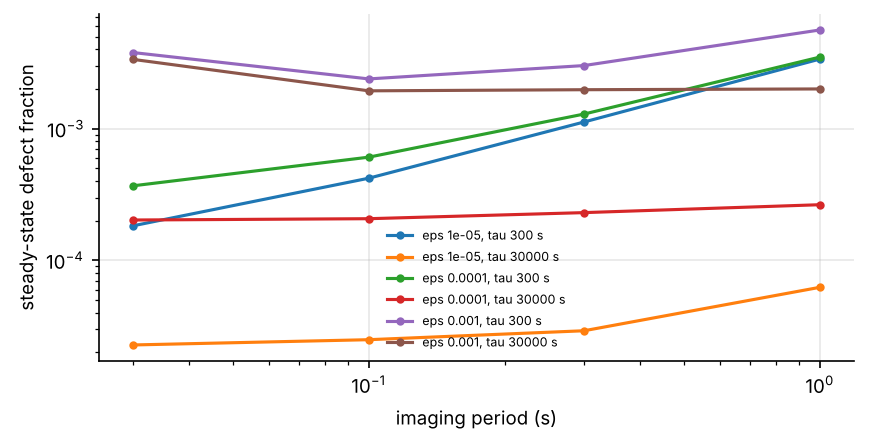
\includegraphics[width=0.8\linewidth]{m25_imaging.png}
\caption{Steady-state defect fraction sampled just after each image versus imaging period, at $10^5$ sites (4~$\times$~4~\textmu m, 85\% loading, 32~$\times$~4 block, intermediate steps, $t_\mathrm{img}=10$~ms, loss $10^{-4}$ per move), for $\epsilon_\mathrm{img}=10^{-5}$, $10^{-4}$, $10^{-3}$ and $\tau=300$ and 30000~s. Each point is one seed, averaged over the second half of a run of $\max(8~\mathrm{s},8T_\mathrm{img})$. The full scan (with $\tau=3000$~s) fits $\rho_\mathrm{image}=2.24\epsilon_\mathrm{img}+0.98(T_\mathrm{img}+t_\mathrm{img})/\tau$; time averages are in Table~\ref{tab:mega-imaging}.}
\label{fig:mega-imaging}
\end{figure}

The time average follows a hole-lifetime model. Let $T=T_\mathrm{img}+t_\mathrm{img}$. An imaging loss is unseen for one period $T$ and is then repaired after a mean delay $d$; a vacuum loss waits $T/2$ on average for the next image, and then $d$. Hence
\begin{equation}
\rho_\mathrm{mean}=\epsilon_\mathrm{img}\,\frac{T+d}{T}+\frac{T/2+d}{\tau}.
\end{equation}
One delay, $d=22$~ms, fits all 40 points at $10^5$ sites with a median error of 9\% ($d=0$ underestimates by a median 16\%). The worst point (41\%) is $\epsilon_\mathrm{img}=10^{-3}$ at $T_\mathrm{img}=30$~ms, where the repair saturates. Minimising $\rho_\mathrm{mean}$ over $T$ gives the optimum imaging period
\begin{equation}
T^*=\sqrt{2\,\epsilon_\mathrm{img}\,d\,\tau}\qquad(d\ll T).
\end{equation}
For $d=22$~ms and $\tau=3000$~s this is 36~ms, 0.11~s and 0.36~s for $\epsilon_\mathrm{img}=10^{-5}$, $10^{-4}$ and $10^{-3}$, in agreement with the minima of the scan (0.03~s, 0.1~s, and a flat minimum between 0.3 and 1~s). At the optimum, $\rho_\mathrm{mean}\approx\epsilon_\mathrm{img}+\sqrt{2\epsilon_\mathrm{img}d/\tau}+d/\tau$; for $\epsilon_\mathrm{img}=10^{-4}$ and $\tau=3000$~s that is $1.5\times10^{-4}$ (simulated $1.4\times10^{-4}$ at $T_\mathrm{img}=0.1$~s). Hence the loss per image dominates the floor once $\tau$ exceeds a few thousand seconds, and lowering $\epsilon_\mathrm{img}$, not imaging more often, is the lever. The imaging time matters only through the dead time at short periods: at $T_\mathrm{img}=30$~ms, $t_\mathrm{img}=3$, 10 and 20~ms give $1.28$, $1.48$ and $1.66\times10^{-4}$.

At $10^6$ sites the delay is not a constant, because the block must sweep its positions to reach a hole (252 for a 32~$\times$~4 block on 4~$\times$~4~\textmu m; a one-pass visit takes 0.9 to 1.0~ms with fast steps and 1.35 to 1.5~ms with intermediate steps). Table~\ref{tab:mega-imaging6} gives the time averages for $\epsilon_\mathrm{img}=10^{-4}$ and $\tau=3000$~s. At $T_\mathrm{img}=30$~ms both timings saturate. The loss rate, $\epsilon_\mathrm{img}/T+1/\tau=2.8\times10^{-3}$ per site per second, needs 2,800 fills per second. At $\rho=2\times10^{-4}$ a block position holds about 0.8 holes, so a sweep of 252 visits (0.25 to 0.4~s) refills only about 200 atoms, while the imaging dead time takes 25\% of the time; the holes pile up until each visit has enough work. By Little's law the mean hole lifetime is $\rho_\mathrm{mean}/(\epsilon_\mathrm{img}/T+1/\tau)$: 0.15~s for fast steps at $T_\mathrm{img}=0.1$~s, and 0.33~s for intermediate steps at both 0.1 and 0.3~s. Intermediate steps at $T_\mathrm{img}=0.3$~s thus reach $2.2\times10^{-4}$, within 15\% of fast steps at 0.1~s, with the 128-engine block and one fifth of the heating per refilled atom (2 against 10~\textmu K). At $10^6$ sites a slower imaging cadence is therefore an alternative to a larger block: the imaging period should match the sweep time of the block rather than be as short as possible.

\begin{table}[htbp]\centering\small
\caption{Time-averaged defect fraction at $10^6$ sites with the 32~$\times$~4 block, $\epsilon_\mathrm{img}=10^{-4}$, $\tau=3000$~s (simulated, \texttt{results/\allowbreak m25\_imaging.json}).}
\label{tab:mega-imaging6}
\begin{tabular}{lccc}
\toprule
timing & $T_\mathrm{img}=0.03$~s & 0.1~s & 0.3~s \\
\midrule
fast (10~\textmu K per move) & $8.7\times10^{-4}$ & $1.9\times10^{-4}$ & $2.0\times10^{-4}$ \\
intermediate (2~\textmu K per move) & $1.5\times10^{-3}$ & $4.1\times10^{-4}$ & $2.2\times10^{-4}$ \\
\bottomrule
\end{tabular}
\end{table}

\subsection{Limits}\label{sec:megascale-limits}

The steady-state model assumes perfect detection apart from the imaging loss, an external reservoir supply, a single objective whose field reaches every site, and one move per refill. It does not schedule the reservoir refresh physically (conveyor timing) and does not include photon scattering. The heating per move is taken from the 1D quantum and 3D classical transport results (Sec.~\ref{sec:transport}), not computed within the steady-state model. The remedy and imaging scans use one seed per case. The tiling result is 1D, with ideal thin lenslets and no surface scatter, and the 24~mm chip edge for a 32~$\times$~8 block is not designed. The static-potential comparison is a first-order budget with an assumed delivery efficiency and cavity buildup. Recommendations follow directly. For $10^4$ sites, one large-field objective or two zones and one 16-chip stack suffice. For $10^5$ sites, a 32~$\times$~4 block, a field of $\pm0.9$~mm or about 13 zones, and about 85\% loading, which cuts the reservoir from two thirds of the sites to a quarter and the static power by 40\%. For $10^6$ sites the transport side is feasible with a block of 128 to 256 engines, but the static potential needs a different source (a cavity lattice or much lower depths), the field needs a lithography-class objective, and the loss rates must improve to reach $10^{-4}$ defects.

\section{Combining stacks and the collimator}\label{sec:combine}

The engine blocks of Sec.~\ref{sec:megascale-remedies} need 32 to 64 rows, i.e.\ two to four 16-chip stacks of the kind described in Sec.~\ref{sec:rows}. A polarising beam splitter combines two stacks; we show here how to combine stacks in space with a slotted mirror at the collimator plane, and then repeat the analysis with the real, traced collimator. The second step changes little for the combiner, but it exposes a limit of the whole stacked relay: a cylindrical collimator at NA 0.9 defocuses the light of tweezers away from the row centre, so a row is usable over only half of its 180~\textmu m segment. We then design an all-reflective collimator that removes this limit. The record is \texttt{docs/\allowbreak megascale.md} (Secs.~11 to 13), \texttt{docs/\allowbreak collimator.md} (Sec.~10), \texttt{scripts/m26\_stack\_combine.py} and \texttt{scripts/m27\_reflective\_collimator.py}.

\subsection{A slotted comb at the collimator plane}\label{sec:combine-comb}

The plane S, formed by the back focal planes of the per-chip collimators, is conjugate to the atoms with magnification $1/D$. Here, $D=125$ for rows 4~\textmu m apart (Sec.~\ref{sec:rows}). At S, each chip's beam is a stripe of $\pm f_\mathrm{FAC}\mathrm{NA}_\mathrm{FAC}=\pm158$~\textmu m on the 0.5~mm chip pitch, so neighbouring beams leave gaps of 184~\textmu m. A mirror with slots, tilted at 45$^\circ$ (a ``comb''), placed in these gaps interleaves two stacks built at twice the chip pitch. Stack A passes through the slots; stack B, turned by 90$^\circ$, is reflected by the teeth. Each beam then sees a window of half-width $a\leq250$~\textmu m. The comb uses no polarisation, and the downstream relay is the same as for a single stack of all the rows. In addition, it doubles the chip pitch to 1.0~mm, which leaves room for the fibre and electrical access that the stacked relay left open (383 fast actuators per engine, 1,532 lines per four-engine chip).

Our choice of a 45$^\circ$ comb is a compromise between two considerations. First, it keeps the optical path of every row of stack B equal to that of stack A: with B's facets in the plane $y=-z_c$, the path to any plane $z=Z$ is $Z$ for all rows. However, the comb then spans the combined stack height along $z$, so the rows at the far end meet it farther from S, where the beams have spread. The question is therefore how far from S a window of half-width $a$ can sit.

\subsection{What sets the comb distance}\label{sec:combine-edge}

We propagate the field of one chip in $y$ from the collimator exit (aperture $f_\mathrm{FAC}$ before S, sine-condition lens, pupil fill $\beta=0.7$~\textmu m, $\mathrm{NA}_\mathrm{FAC}=0.9$) to the comb at a distance $z$ from S, apply the window, propagate back to S, and continue to the atoms through the pupil (\texttt{picsim/opa/stack.RelayY}, \texttt{results/\allowbreak m26\_edge.json}). Without a comb this reproduces the earlier stacked-relay values (transmission 0.973, crosstalk at 4~\textmu m $1.09\times10^{-4}$ against $1.06\times10^{-4}$). Table~\ref{tab:combine-edge} and Fig.~\ref{fig:combine-edge} give the penalty for a single tweezer.

\begin{table}[htbp]\centering\small
\caption{Comb penalty versus distance $z$ from S, single tweezer, 1D in $y$, ideal thin collimator with a hard edge, slot window of half-width $a$ (simulated, \texttt{results/\allowbreak m26\_edge.json}). Loss is the power clipped by the comb (\%); peak is relative to no comb; crosstalk (xt) to the neighbouring row at 4 and 3~\textmu m, in units of $10^{-4}$.}
\label{tab:combine-edge}
\begin{tabular}{lccccccc}
\toprule
 & \multicolumn{4}{c}{$a=250$~\textmu m} & \multicolumn{3}{c}{$a=225$~\textmu m} \\
$z$ from S & loss & peak & xt 4~\textmu m & xt 3~\textmu m & loss & peak & xt 4~\textmu m \\
\midrule
no comb & 0 & 1 & 1.1 & 2.9 & 0 & 1 & 1.1 \\
10~mm & $<0.1\%$ & 0.998 & 1.0 & 2.8 & 0.06\% & 0.992 & 1.1 \\
20~mm & 0.25\% & 0.992 & 1.5 & 4.0 & 0.72\% & 0.985 & 1.8 \\
30~mm & 0.85\% & 0.987 & 2.7 & 7.1 & 1.6\% & 0.981 & 3.1 \\
45~mm & 1.9\% & 0.973 & 6.0 & 17 & 3.4\% & 0.956 & 7.9 \\
60~mm & 3.6\% & 0.953 & 13 & 29 & 5.3\% & 0.931 & 16 \\
\bottomrule
\end{tabular}
\end{table}

\begin{figure}[htbp]\centering
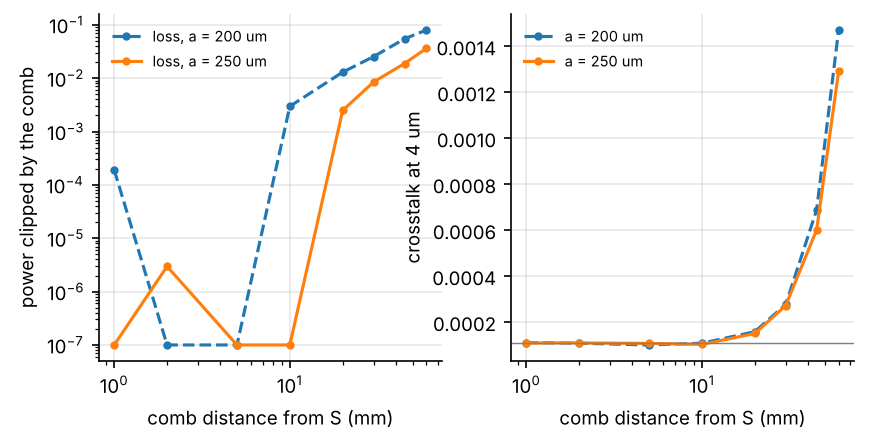
\includegraphics[width=0.8\linewidth]{m26_edge.png}
\caption{Comb penalty versus distance of the comb from S, single tweezer, 1D wave optics in $y$ (ideal thin sine-condition collimator, $\beta=0.7$~\textmu m, $\mathrm{NA}_\mathrm{FAC}=0.9$, hard edge, NA 0.5 pupil), for slot windows of half-width $a=200$~\textmu m (dashed) and 250~\textmu m (solid). Left: power clipped by the comb (values below $10^{-7}$ drawn at $10^{-7}$). Right: crosstalk to the neighbouring row at 4~\textmu m; grey line, without comb. The rise sets in near $z_\mathrm{max}=(a-f_\mathrm{FAC}\mathrm{NA}_\mathrm{FAC})D/\mathrm{NA}$.}
\label{fig:combine-edge}
\end{figure}

The hard edge of the collimator is not the problem. Its Fresnel tail spreads into the gap, but it consists of directions steeper than the pupil accepts, and clipping it costs nothing. A Fresnel-tail estimate that ignores the pupil predicts 0.36\% loss at 10~mm; the simulated loss there is below 0.1\%. A graded collimator edge (raised cosine from 0.8 to 0.9 of the aperture) therefore does not help: it raises the baseline crosstalk to $1.5\times10^{-4}$ and gains no distance. What matters is the light inside the pupil acceptance, which leaves S at half-angle $\mathrm{NA}/D=4$~mrad. It reaches the window edge at
\begin{equation}
z_\mathrm{max}=\frac{(a-f_\mathrm{FAC}\mathrm{NA}_\mathrm{FAC})\,D}{\mathrm{NA}},
\label{eq:zmax}
\end{equation}
which is 23~mm for $a=250$~\textmu m and 17~mm for $a=225$~\textmu m. This agrees with the scan: at $z=20$~mm and $a=250$~\textmu m the worst row loses 0.25\% and the crosstalk at 4~\textmu m rises from $1.1\times10^{-4}$ to $1.5\times10^{-4}$, while at 30~mm it reaches $2.7\times10^{-4}$. A single edge, as used for block combining (rows 0 to 15 from one stack and 16 to 31 from the other), behaves similarly. It also shifts the boundary row by 1.7~nm at $z=20$~mm ($a=250$~\textmu m) and by 12~nm at $a=200$~\textmu m, a static offset to calibrate. The rows are mutually incoherent (\texttt{docs/\allowbreak row\_coherence.md}), so this crosstalk adds in intensity.

\subsection{Layouts for 32 to 64 rows}\label{sec:combine-layouts}

Table~\ref{tab:combine-layout} lists the layouts (\texttt{results/\allowbreak m26\_layout.json}). We place the first comb point at $z_c=7.0$~mm, 0.5~mm (a choice) beyond the $x$ slit plane of the traced $x$ lens and collimator (Sec.~\ref{sec:combine-lens}), and the worst row is the one at the far end of the comb. Two 16-chip stacks at 1.0~mm pitch need a comb from 7 to 23~mm, which ends at $z_\mathrm{max}$; their worst row loses 0.45\% of its power, with peak 0.991 and crosstalk $1.8\times10^{-4}$ at 4~\textmu m. Two such pairs, combined by a polarising beam splitter (PBS), give 64 rows at the same penalty. Combining only by comb with longer stacks puts the far rows beyond $z_\mathrm{max}$ (7 to 31~mm for 24-chip stacks, 7 to 39~mm for 32-chip stacks) and costs up to 1.3\% and $3.9\times10^{-4}$. A second comb level (stacks at 2.0~mm, combined pairwise and then again) would put the second comb beyond $z_\mathrm{max}$, so we do not use it. With $a=225$~\textmu m, which is about what a 50~\textmu m tooth plate ($t/(2\sqrt{2})=18$~\textmu m per edge) and $\pm10$~\textmu m edge placement leave, the worst rows of the two preferred layouts lose 0.86\% and reach $2.0\times10^{-4}$.

\begin{table}[htbp]\centering\small
\caption{Layouts for 32 to 64 rows (simulated and derived, \texttt{results/\allowbreak m26\_layout.json}; first comb point at $z_c=7$~mm). Worst row at $a=250$~\textmu m: power loss, peak and crosstalk at 4~\textmu m (units of $10^{-4}$). The last column states whether the objective must accept both polarisations. Bold: preferred layouts.}
\label{tab:combine-layout}
\setlength{\tabcolsep}{4pt}
\begin{tabular}{lllccccc}
\toprule
 & & chips per & comb & \multicolumn{3}{c}{worst row} & pol.-insensitive \\
rows & layout & stack, pitch & $z$ range & loss & peak & xt 4~\textmu m & objective \\
\midrule
32 & one stack & 32, 0.5~mm & & \multicolumn{3}{c}{(no comb)} & no \\
32 & 2 stacks, PBS & 16, 0.5~mm & & \multicolumn{3}{c}{(no comb)} & yes \\
32 & \textbf{2 stacks, comb} & \textbf{16, 1.0~mm} & \textbf{7--23~mm} & \textbf{0.45\%} & \textbf{0.991} & \textbf{1.8} & \textbf{no} \\
48 & 4 stacks, comb + PBS & 12, 1.0~mm & 7--19~mm & 0.21\% & 0.992 & 1.4 & yes \\
48 & 2 stacks, comb & 24, 1.0~mm & 7--31~mm & 0.93\% & 0.987 & 2.9 & no \\
64 & \textbf{4 stacks, comb + PBS} & \textbf{16, 1.0~mm} & \textbf{7--23~mm} & \textbf{0.45\%} & \textbf{0.991} & \textbf{1.8} & \textbf{yes} \\
64 & 2 stacks, comb & 32, 1.0~mm & 7--39~mm & 1.3\% & 0.984 & 3.9 & no \\
64 & 2 stacks, PBS & 32, 0.5~mm & & \multicolumn{3}{c}{(no comb)} & yes \\
\bottomrule
\end{tabular}
\end{table}

A single taller stack (32 or 64 chips at 0.5~mm) needs no combiner. In first-order optics it only enlarges the $y$-relay field, to $\pm8$ or $\pm16$~mm at the first telescope lens and 3.7 or 7.4~mrad at the pupil. Its costs are mechanical: 16 to 32~mm of facets flush to about 100~\textmu m, and all the input and output lines at 0.5~mm pitch.

\paragraph{2D check.} The 1D model leaves out the circular pupil, which couples $x$ and $y$, and the full rows. We therefore pass the comb-windowed $y$ pupil of both chips through the 2D model of the stacked relay (D1 $x$ response, circular NA 0.5 pupil; \texttt{results/\allowbreak m26\_twod.json}). Chip $m$ forms a full row of 41 tweezers at 3~\textmu m, chip $m+1$ forms 11 tweezers offset by 1.5~\textmu m, and one tweezer of chip $m$ then moves by 0.25~\textmu m. Without a comb this reproduces the earlier 2D values. Table~\ref{tab:combine-2d} shows that 2D does not change the conclusions. At the worst row the full-row crosstalk rises by a factor 1.3, and the effect of a moving tweezer on the next row by a factor 1.55 to 1.65 (to $3.9\times10^{-5}$ in depth at 4~\textmu m, $9.6\times10^{-5}$ at 3~\textmu m). This is still more than an order of magnitude below the in-row figures of D1 (0.11\%, 3.5~nm). Tweezers at $x=0$ and at the row end (60~\textmu m) give the same values to 0.1\%, because the comb acts on $y$ alone and the circular pupil couples the two axes only weakly. The 1D single-tweezer crosstalk ($1.8\times10^{-4}$ at $z=23$~mm) slightly overstated the 2D one ($1.5\times10^{-4}$). The block-combining edge moves the boundary row by 7~nm in 2D (peak position), a static offset to calibrate. With coherent rows the comb would raise the static depth change at 4~\textmu m from 2.6\% to 2.9\%; rows must stay incoherent, as they must without a comb.

\begin{table}[htbp]\centering\small
\caption{2D check of the comb (simulated, \texttt{results/\allowbreak m26\_twod.json}; both chips windowed, rows incoherent). Crosstalk (xt) and the relative change of the neighbour row's trap depth in units of $10^{-4}$; neighbour row at 4~\textmu m, at 3~\textmu m in brackets.}
\label{tab:combine-2d}
\setlength{\tabcolsep}{4pt}
\begin{tabular}{lccccc}
\toprule
 & \multicolumn{2}{c}{single tweezer} & full row & \multicolumn{2}{c}{neighbour depth change} \\
comb & peak & xt 4~\textmu m & xt 4~\textmu m, max over $x$ & static & moving tweezer \\
\midrule
none & 1 & 1.1 & 1.8 & 1.7 (2.0) & 0.24 (0.62) \\
$z$ 15~mm, $a$ 250~\textmu m & 0.995 & 1.1 & 1.8 & 1.8 (2.2) & 0.29 (0.74) \\
$z$ 23~mm, $a$ 250~\textmu m (worst row) & 0.990 & 1.5 & 2.3 & 2.1 (2.6) & 0.39 (0.96) \\
$z$ 23~mm, $a$ 225~\textmu m & 0.982 & 1.6 & 2.4 & 2.2 (2.2) & 0.39 (0.80) \\
$z$ 30~mm, $a$ 250~\textmu m ($>z_\mathrm{max}$) & 0.984 & 2.1 & 2.9 & 2.5 (3.1) & 0.53 (1.2) \\
single edge, $z$ 23~mm, $a$ 250~\textmu m & 0.995 & 1.3 & 2.0 & 1.9 (2.2) & 0.34 (0.84) \\
\bottomrule
\end{tabular}
\end{table}

\paragraph{Tolerances.} The tolerances follow from the conjugations and the decentre results of the stacked relay (derived). A comb tilt $\theta$ about $x$ deflects stack B by $2\theta$ at S. This shifts its facet image in the pupil by $2\theta F_y$, with $F_y=2.17$~m, which gives 1\% peak loss at $\theta=0.16$~mrad and 3\% at 0.28~mrad. The same tilt moves B's rows by $2\theta z/D$: 0.32~nm per \textmu rad at $z=20$~mm, and 50~nm at 0.16~mrad. This static offset alternates between rows, because A and B rows interleave, so it must be calibrated once against the static array; keeping the alternating pitch error below 3~nm then needs a tilt stability of about 10~\textmu rad (drift, not alignment; mount stability not yet checked against a source [REF?]). Moving the comb by $\mathrm{d}z$ along $z$ changes B's path by $\mathrm{d}z$, which tolerates 100~\textmu m (chip piston, peak $\geq0.992$); it also shifts the windows by $\mathrm{d}z$ in $y$, which should stay within about $\pm10$~\textmu m. Light that misses a tooth leaves at 90$^\circ$ to a dump; light from stack A that hits the back of a tooth is reflected towards stack B and needs an absorbing back face.

\paragraph{Comb roll.} A comb edge that is not parallel to $x$ makes the window depend on $x$. Beyond the slit plane the $x$ relay is telecentric, so each tweezer meets the comb at its slit-plane position $X=f_1 s$, and four engines at 3.0~mm pitch span $X=\pm5.6$~mm. One tweezer's footprint at the comb is at most $\pm0.78$~mm (17~mm beyond the slit plane, half-angle $(A/2)/f_1=0.046$). Hence, for a roll of 2~mrad, the edge moves by only 3~\textmu m across one tweezer, against the tens of \textmu m over which the result changes, and we treat each tweezer with its local window $a(X)$. In 2D at $z=23$~mm the peak falls from 0.989 to 0.972 as $a$ goes from 250 to 205~\textmu m (about 0.04\% per \textmu m), while the crosstalk at 4~\textmu m stays at 1.4 to $1.6\times10^{-4}$. A roll therefore mainly makes the depth vary along the row, by about $\pm0.4\%$ for a $\pm10$~\textmu m change of $a$, which a 1.8~mrad roll produces over $\pm5.6$~mm. The engines set each tweezer's power in any case, so this is a calibration, not a limit; the same holds for an edge straightness of $\pm10$~\textmu m over 12~mm.

Thus the blocks of Sec.~\ref{sec:megascale} can be built as follows. (i) For 32 rows, two 16-chip stacks at 1.0~mm pitch and one comb. This needs no polarisation optics, and since alternate rows come from different stacks, the passive orthogonal-polarisation decorrelation of \texttt{docs/\allowbreak row\_coherence.md} comes for free if the objective accepts it. (ii) For 64 rows, two such comb pairs combined by a PBS. Four 16-chip stacks with four engines per chip at 3.0~mm pitch (12~mm edge) then form the 64~$\times$~4 block, with 256 engines and 98,048 fast actuators. With intermediate steps at $10^6$ sites it reaches a time average of $2.9\times10^{-4}$ on 4~$\times$~4~\textmu m and $2.7\times10^{-4}$ on 3~$\times$~4~\textmu m, without the 24~mm chip edge that 32~$\times$~8 needs. The worst rows lose 0.9 to 1.5\% of their peak depth to the comb ($a=250$ / 225~\textmu m), which the per-tweezer power set by the engines recovers. The edge scan is 1D in $y$ and the 2D check uses the same windowed pupil; both take the window of each slot at one distance $z$, whereas the 45$^\circ$ tilt places the two edges of a 0.5~mm slot 0.25~mm before and after that distance, which changes $z$ by at most 4\% at $z_c=7$~mm. Tooth-edge roughness, scatter from the comb and a lens design of the larger $y$-relay field are not included.

\subsection{The comb with the real collimator}\label{sec:combine-lens}

The analysis above used an ideal thin collimator in air. The adopted collimator is a fused-silica Weierstrass block glued to the facet, followed by a 10~\textmu m gap and a 250~\textmu m aplanat of index 1.8 (\texttt{docs/\allowbreak collimator.md}). We repeat the comb study with this traced lens (\texttt{results/\allowbreak m26\_lens.json}). The exit field is built from the traced lens map (exit height, wavefront and amplitude per ray) at a plane 60~\textmu m beyond the last vertex, and S lies at the traced back focal plane, 0.44~mm from the facet. Without a comb this reproduces the wave model of the traced collimator: crosstalk $8.0\times10^{-5}$ at 4~\textmu m against $8.4\times10^{-5}$, and $3.8\times10^{-4}$ against $4.0\times10^{-4}$ at 3~\textmu m. The real geometry also moves the comb. The traced $x$ lens puts the $x$ slit plane 6.76~mm from the facet, the collimator glass adds 0.15~mm in $x$ ($t(1-1/n)$ per section), and we keep 0.5~mm of clearance; the comb therefore starts 7.0~mm from S, and the far row of a 32-row comb sits at 23.0~mm.

\begin{table}[htbp]\centering\small
\caption{Comb penalty with the real (traced) collimator against the ideal thin collimator, slot window $a=250$~\textmu m, 1D (simulated, \texttt{results/\allowbreak m26\_lens.json}). Values for $a=225$~\textmu m are given in the text.}
\label{tab:combine-lens}
\setlength{\tabcolsep}{4pt}
\begin{tabular}{lcccccc}
\toprule
 & \multicolumn{3}{c}{real collimator} & \multicolumn{3}{c}{thin collimator} \\
$z$ from S & loss & peak & xt 4~\textmu m & loss & peak & xt 4~\textmu m \\
\midrule
15~mm & $5\times10^{-4}$ & 0.994 & $7.6\times10^{-5}$ & $5\times10^{-4}$ & 0.994 & $1.2\times10^{-4}$ \\
20~mm & $2.6\times10^{-3}$ & 0.991 & $9.2\times10^{-5}$ & $2.5\times10^{-3}$ & 0.992 & $1.5\times10^{-4}$ \\
23.0~mm (far row) & $5.0\times10^{-3}$ & 0.991 & $1.1\times10^{-4}$ & $4.5\times10^{-3}$ & 0.991 & $1.8\times10^{-4}$ \\
30~mm & $9.0\times10^{-3}$ & 0.988 & $1.9\times10^{-4}$ & $8.5\times10^{-3}$ & 0.987 & $2.7\times10^{-4}$ \\
\bottomrule
\end{tabular}
\end{table}

As can be seen from Table~\ref{tab:combine-lens}, the immersed facet puts more light near the edge of the beam at S, but loss and peak follow the thin-lens values within 12\%, and the crosstalk is lower. With $a=225$~\textmu m the real collimator gives loss / peak / crosstalk at 4~\textmu m of $3.4\times10^{-3}$ / 0.986 / $7.5\times10^{-5}$ at 15~mm, $7.6\times10^{-3}$ / 0.985 / $9.7\times10^{-5}$ at 20~mm, $9.3\times10^{-3}$ / 0.986 / $1.2\times10^{-4}$ at the far row and $1.7\times10^{-2}$ / 0.983 / $2.0\times10^{-4}$ at 30~mm. Equation~\eqref{eq:zmax} therefore still holds. In 2D at the far row ($z=23.0$~mm, $a=250$~\textmu m), the full-row crosstalk at 4~\textmu m is $1.6\times10^{-4}$ ($1.75\times10^{-4}$ without the comb). A moving tweezer changes the next row by $2.8\times10^{-5}$ in depth at 4~\textmu m ($1.2\times10^{-5}$ without the comb) and by $6.9\times10^{-5}$ at 3~\textmu m ($3.6\times10^{-5}$). Hence the comb conclusions hold for the real collimator in the real geometry.

\subsection{Skew rays: light that leaves the chip at an angle along \texorpdfstring{$x$}{x}}\label{sec:combine-skew}

A tweezer at position $x_a$ along the row is formed by light that leaves the emitters with $x$ direction sine $s_x=x_a/x_\mathrm{scale}$. Here, $x_\mathrm{scale}=288$~\textmu m for D1, so $s_x$ reaches 0.31 at the end of a 180~\textmu m segment and 0.355 at the slit edge. The collimator is cylindrical: its surface normals have no $x$ component, so $k_x$ is conserved, and the $y$-$z$ problem is exactly the 2D trace with every index $n$ replaced by the effective index
\begin{equation}
n_\mathrm{eff}=\sqrt{n^2-s_x^2}.
\end{equation}
A unit test checks this against 3D vector refraction. All earlier $y$ models (the stacked relay, the traced collimator, and the comb study above) used $s_x=0$. For $s_x>0$ the effective index ratios of the lens rise, from 1.45 to 1.50 for the block and from 1.80 to 1.89 for the aplanat at $s_x=0.355$, and the lens is no longer aplanatic for the facet (\texttt{results/\allowbreak m26\_skew.json}). Table~\ref{tab:combine-skew} and Fig.~\ref{fig:combine-skew} give the result.

\begin{table}[htbp]\centering\small
\caption{Tweezer at $x_a$ with the adopted collimator, relative to an ideal collimator at the same $s_x$ (simulated, \texttt{results/\allowbreak m26\_skew.json}; effective-index trace, downstream relay ideal, no comb; with the comb at the far row the crosstalk changes by a factor 0.9 to 1.6). Peak in 1D (2D in brackets), equivalent facet focus error, residual wavefront after refocusing the facet for this tweezer, and crosstalk at 4~\textmu m.}
\label{tab:combine-skew}
\begin{tabular}{lcccc}
\toprule
$x_a$ ($s_x$) & peak & equivalent facet defocus & residual after refocusing & xt 4~\textmu m \\
\midrule
0 & 1.000 (1.000) & 0 & 0 & $8.4\times10^{-5}$ \\
15~\textmu m (0.052) & 0.999 (0.997) & $-0.27$~\textmu m & 0.001 waves & $2.2\times10^{-4}$ \\
30~\textmu m (0.104) & 0.971 (0.942) & $-1.10$~\textmu m & 0.005 waves & $3.0\times10^{-3}$ \\
45~\textmu m (0.156) & 0.794 (0.725) & $-2.46$~\textmu m & 0.014 waves & $8.2\times10^{-3}$ \\
60~\textmu m (0.208) & 0.481 (0.440) & $-4.36$~\textmu m & 0.029 waves & $6.9\times10^{-3}$ \\
90~\textmu m (0.312) & 0.231 & $-9.67$~\textmu m & 0.096 waves & $9.0\times10^{-3}$ \\
\bottomrule
\end{tabular}
\end{table}

\begin{figure}[htbp]\centering
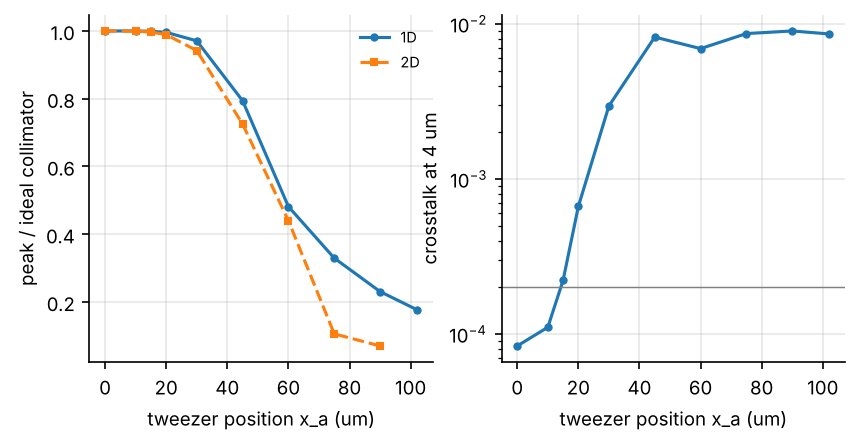
\includegraphics[width=0.8\linewidth]{m26_skew.png}
\caption{Effect of the $x$ direction sine $s_x=x_a/288$~\textmu m on the adopted cylindrical collimator (glued fused-silica Weierstrass block and 250~\textmu m aplanat of index 1.8, NA 0.9), traced with effective indices $\sqrt{n^2-s_x^2}$, with an ideal downstream relay, no comb and no facet focus offset. Left: peak of a tweezer at $x_a$ relative to an ideal collimator at the same $s_x$, 1D (solid) and 2D with the circular NA 0.5 pupil (dashed). Right: crosstalk at 4~\textmu m to the neighbouring row (1D); grey line at $2\times10^{-4}$ for reference.}
\label{fig:combine-skew}
\end{figure}

The error is almost purely a focus shift of the facet,
\begin{equation}
\Delta z\approx-99\,s_x^2~\text{\textmu m}.
\end{equation}
A thin glass lens in air would give $-f(n+1)s_x^2/(2n)=-148\,s_x^2$~\textmu m, the same order. Refocusing the facet for one tweezer restores its peak fully; the residual after refocusing stays below 0.1 waves up to 90~\textmu m. However, all tweezers of a row share the facet and the collimator. The phase error sits at S, which is conjugate to the atoms, so refocusing the atom plane does not help either. In 2D the best atom-plane focus recovers the peak up to $x_a=30$~\textmu m (1.02), but with a 1.5~\textmu m $y$-focus shift, outside the $\pm0.5$~\textmu m axial registration of the transport model (Sec.~\ref{sec:transport}), and not beyond. The 2D model covers $|x_a|\leq60$~\textmu m only: its engine (D1, 128 ports) cannot form a tweezer beyond about 67~\textmu m for any collimator.\footnote{An earlier version read the 2D values at 75 and 90~\textmu m (peak 0.11 at 75~\textmu m) as a break-up of the spot in the circular pupil. They are outside the model; the 1D results, which do not involve the engine, hold to the slit edge.}

\paragraph{What a common focus offset recovers.} A single facet offset for the whole row, i.e.\ the length of the glued block set at fabrication, trades the centre against the ends (\texttt{results/\allowbreak m26\_skew\_offset.json}, first-order focus phase, 1D). With $\Delta z=-1.25$~\textmu m the peak stays at or above 0.96 out to $|x_a|=45$~\textmu m, and the static crosstalk at 4~\textmu m stays at or below $3.6\times10^{-3}$. That is within the criteria of \texttt{docs/\allowbreak row\_coherence.md} (others' depth change below $3\times10^{-3}$ when a tweezer moves), since for incoherent rows the moving-tweezer effect was about 0.13 of the static crosstalk in the earlier stacked-relay model; we did not recompute it for skewed tweezers. Beyond 50~\textmu m no offset helps: the peak is 0.90 at 50~\textmu m and 0.66 at 60~\textmu m, and no offset brings the worst peak over $|x_a|\leq90$~\textmu m above 0.43.

\paragraph{Consequences.} A refractive cylindrical collimator at NA 0.9 serves about half of the 180~\textmu m segment ($|x_a|\leq45$~\textmu m, about 23 sites at 4~\textmu m), not all of it. Every power and crosstalk figure of the stacked relay, of the traced collimator and of the comb study above holds near the row centre and is optimistic for the outer half. For the large arrays of Sec.~\ref{sec:megascale} this doubles the number of engines per row at fixed coverage (90~\textmu m segments instead of 180~\textmu m). The alternative is a collimator that is insensitive to $s_x$. Serving $|x_a|\leq90$~\textmu m within the $\pm0.5$~\textmu m focus tolerance, with the best common offset, needs $|\Delta z/s_x^2|\leq10$~\textmu m, ten times less than now. The all-reflective collimator of Sec.~\ref{sec:combine-reflective} meets this with $\Delta z=0$.

We see four routes. (i) An all-reflective collimator in one medium. The law of reflection and a uniform medium are unchanged by the effective-index map, so the wavefront error vanishes for every $s_x$, and a flat exit face normal to the collimated beam keeps it so (derived). It needs a folded geometry within the 0.5~mm chip pitch; we design it in Sec.~\ref{sec:combine-reflective}. (ii) A cemented refractive design. Glass-glass interfaces are less sensitive than glass-air ones (relative power change $0.41\,s_x^2$ for a 1.45 to 2.0 interface against $0.84\,s_x^2$ for 1.45 to air, derived), but a factor of two is not enough on its own. (iii) A corrector at the $x$ slit plane, where $x$ encodes $s_x$. This fails at large $s_x$: at $x_a=90$~\textmu m the error acts at S like a $y$ lens of 4~mm focal length (2.9 waves at 158~\textmu m), so the beam has passed a focus before it reaches the slit plane, 6.5~mm later. (iv) A larger vertical facet mode, i.e.\ a lower facet NA. This helps by less than a factor of two, because the optimal pupil fill, and with it $f_\mathrm{FAC}$, grows with the mode. Of these, only the reflective route removes the error in principle. The downstream cylindrical lenses of the $y$ relay see $x$ angles below about 0.05 and are not modelled; the skew trace is exact for cylindrical surfaces, but the downstream relay is taken as ideal, and the common-offset result uses a first-order focus phase in 1D.

\subsection{An all-reflective collimator}\label{sec:combine-reflective}

\paragraph{Why two mirrors.} A mirror in one medium keeps the wavefront flat at every $s_x$, as argued above. One mirror (an off-axis parabola) collimates, but maps the far field with a strongly asymmetric distortion for a cone of $\pm38^\circ$ in glass. Two mirrors designed together can meet two conditions, exact collimation and the sine condition in the medium, $y_S-y_c=\pm nf\sin\theta$. Here, $\theta$ is the ray angle in the glass, $y_c$ the centre of the collimated beam and $f=175$~\textmu m. Under the effective-index map such a pair stays aplanatic. Only its focal length changes, to $fn/n_\mathrm{eff}$, i.e.\ by 3.1\% at the slit edge in fused silica (7\% in air). The stripe edge at S does not move, because the rim of the first mirror fixes $\theta$ (derived).

\paragraph{Construction and selection.} We construct the pair as the refractive aplanat of Sec.~\ref{sec:rows-collimator} is constructed (Wassermann-Wolf in 2D), with mirrors. The first mirror M1 is $r(\theta)(\sin\theta,\cos\theta)$ from the facet. The direction after M1 follows in closed form from a constant optical path to a plane, the law of reflection gives $r'=r\cot[(\phi-\theta)/2]$, and the second mirror M2 then sends every ray along $z$ (\texttt{picsim/\allowbreak opa/\allowbreak mirror\_collimator.py}). We scanned 3,780 constructions over the distance of M1, the beam centre, the fold angle and the mapping orientation (\texttt{results/\allowbreak m27\_scan.json}). We kept those with no light behind the facet plane, no obscuration, a radius of curvature of at least 20~\textmu m, and no overlap between the blocks of neighbouring chips at 0.5~mm pitch, with 10~\textmu m clearance around each block's light. 290 layouts pass. A normal displacement $\delta$ of a back-surface mirror in glass changes the path by $2n\cos i\,\delta$. Over the passing layouts this sensitivity is 2.1 to 3.2, rms over the pupil (against 0.45 to 0.8 for a refracting surface of the adopted design), and grazing folds are the least sensitive but the longest. We adopted the least sensitive layout no longer than 0.5~mm, a choice comparable to the 0.40~mm refractive collimator.

\begin{table}[htbp]\centering\small
\caption{Adopted all-reflective collimator (simulated, \texttt{results/\allowbreak m27\_scan.json}, \texttt{m27\_trace.json}, \texttt{m27\_wave.json}, \texttt{m27\_tolerance.json}). Fused silica ($n=1.4496$) glued to the facet; $f=175$~\textmu m, NA~0.9; on-axis wave-model figures at $\beta=0.7$~\textmu m.}
\label{tab:combine-refl}
\begin{tabular}{ll}
\toprule
quantity & value \\
\midrule
M1 distance on axis / beam centre / axial fold & 50~\textmu m / $-390$~\textmu m / $-70^\circ$ \\
block length (facet to exit face) / glass path of the axial ray & 476~\textmu m / 749~\textmu m \\
$y$ extent of the light / largest cross-section & $-547$ to $+17$~\textmu m / 315~\textmu m \\
incidence on M1 / on M2 (critical angle $43.6^\circ$) & $28$ to $77^\circ$ / $44.6$ to $60.0^\circ$ (TIR) \\
smallest radius of curvature, M1 / M2 & 193 / 798~\textmu m \\
wavefront, 3D trace, $s_x\leq0.355$ & $<2\times10^{-12}$ waves p-v \\
peak per guided power / $y$ FWHM / crosstalk at 4~\textmu m ($s_x=0$) & 1.10 / 1.35~\textmu m / $8\times10^{-5}$ \\
mirror-pair reflectance, M1 silver / gold, M2 TIR & 0.996 / 0.982 \\
laser power per 1.2~mK tweezer, M1 silver & 57.7~mW \\
facet decentre / focus for $\leq3\%$ loss & $\pm0.1$ / $\pm1$~\textmu m \\
mirror form error for $\leq2\%$ loss & $\leq10$~nm rms \\
\bottomrule
\end{tabular}
\end{table}

\begin{figure}[htbp]\centering
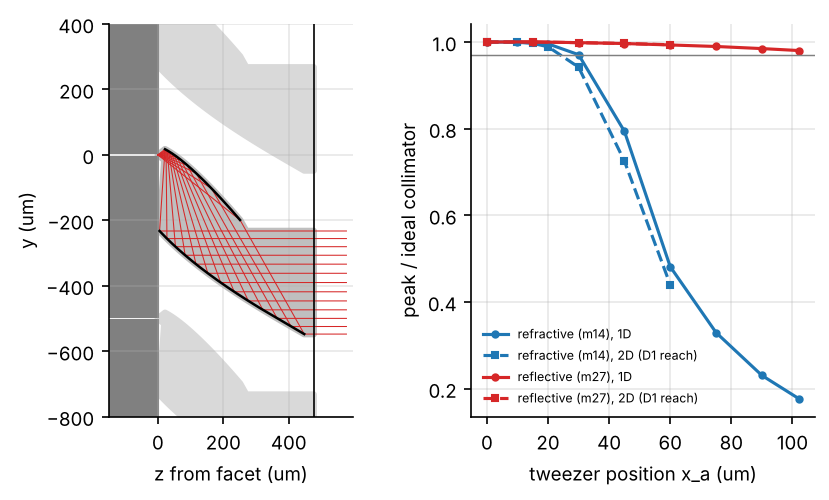
\includegraphics[width=0.95\linewidth]{m27_figure.png}
\caption{Left: $y$-$z$ section of the adopted all-reflective collimator, from the facet (origin) to the flat exit face (vertical line), with rays every $6.4^\circ$ in the glass; mirrors in black. Grey: light regions, with 10~\textmu m margin, of the blocks of the neighbouring chips at $\pm0.5$~mm; dark grey: the chips ($z<0$). Right: peak of a tweezer at $x_a$ relative to an ideal collimator at the same $s_x$ (effective-index trace, verified by a 3D vector trace; downstream relay ideal), for the refractive collimator of Sec.~\ref{sec:combine-skew} (blue) and the reflective one (red); 1D to the slit edge, 2D only within the 67~\textmu m reach of the D1 engine of the 2D model.}
\label{fig:combine-refl}
\end{figure}

\paragraph{Exactness.} We traced the adopted design independently, in 3D, with rays launched with $k_x$ (not with the effective index), the vector law of reflection on spline fits of the two mirror curves, and the optical path as $n$ times the 3D length (\texttt{results/\allowbreak m27\_trace.json}). At $s_x=0$, 0.1, 0.2, 0.312 and 0.355 the phase of the $k_x=k_0s_x$ component is flat to $2\times10^{-12}$ waves, the exit height equals $fs\,n/n_\mathrm{eff}$ to $2\times10^{-10}$, and the 2D effective-index lens map used by the wave model agrees with the 3D trace. The refractive collimator carries 0.30, 1.18, 2.86 and 3.67 waves p-v at the same $s_x$.

\paragraph{Performance.} On axis the reflective collimator equals the refractive one to four digits in the wave model (\texttt{results/\allowbreak m27\_wave.json}). Across the row it holds the peak and the crosstalk (Table~\ref{tab:combine-refl-skew}, Fig.~\ref{fig:combine-refl}; \texttt{results/\allowbreak m27\_skew.json}). The remaining 1.5\% at 90~\textmu m is the 2.4\% longer focal length; relative to its own centre the tweezer keeps 0.990. The $y$ centroid does not move, because the mapping stays antisymmetric. Hence one engine serves its whole 180~\textmu m segment without a common focus offset, and the doubling of engines discussed above is not needed.

\begin{table}[htbp]\centering\small
\caption{Tweezer at $x_a$ with the reflective and the refractive collimator, relative to an ideal collimator at the same $s_x$ (simulated, \texttt{results/\allowbreak m27\_skew.json} and \texttt{m26\_skew.json}). Peak in 1D (2D in brackets, within the reach of the D1 engine), crosstalk at 4~\textmu m, and the loss of the comb at the far row of a 32-row block ($a=250$~\textmu m, 23.5~mm from S for the reflective design).}
\label{tab:combine-refl-skew}
\setlength{\tabcolsep}{4pt}
\begin{tabular}{lccccc}
\toprule
 & \multicolumn{2}{c}{peak} & \multicolumn{2}{c}{xt 4~\textmu m} & comb loss \\
$x_a$ & reflective & refractive & reflective & refractive & reflective \\
\midrule
0 & 1.000 (1.000) & 1.000 (1.000) & $8.4\times10^{-5}$ & $8.4\times10^{-5}$ & $4.8\times10^{-3}$ \\
30~\textmu m & 0.999 (0.999) & 0.971 (0.942) & $8.4\times10^{-5}$ & $3.0\times10^{-3}$ & $4.9\times10^{-3}$ \\
45~\textmu m & 0.997 (0.997) & 0.794 (0.725) & $8.6\times10^{-5}$ & $8.2\times10^{-3}$ & $5.0\times10^{-3}$ \\
60~\textmu m & 0.993 (0.994) & 0.481 (0.440) & $9.0\times10^{-5}$ & $6.9\times10^{-3}$ & $5.1\times10^{-3}$ \\
90~\textmu m & 0.985 & 0.231 & $9.7\times10^{-5}$ & $9.0\times10^{-3}$ & $5.4\times10^{-3}$ \\
102~\textmu m (slit edge) & 0.980 & 0.177 & $1.0\times10^{-4}$ & $8.6\times10^{-3}$ & $5.5\times10^{-3}$ \\
\bottomrule
\end{tabular}
\end{table}

\paragraph{The $x$ axis and the comb.} The folded glass path (749~\textmu m on axis) moves S and the $x$ slit plane (\texttt{results/\allowbreak m27\_xaxis.json}). The comb then starts 7.51~mm from S, and the far row of a 32-row comb sits at 23.5~mm instead of 23.0~mm, with the losses of Table~\ref{tab:combine-refl-skew}. After its defocus is absorbed by placing the $x$ lens, the glass adds 0.47 waves p-v of higher-order phase in $s_x$. Before recalibration this costs D1 tweezers at $\pm60$~\textmu m less than $3\times10^{-4}$ in peak and 1.4~nm in position; after recalibration nothing measurable remains.

\paragraph{Costs.} The design has three costs, in order of weight.

(i) Form tolerance (\texttt{results/\allowbreak m27\_tolerance.json}). In a Monte Carlo of random mirror form errors (24 samples, correlation 20 and 60~\textmu m), 10~nm rms costs 1.2\% in mean peak (10th percentile 1.7 to 1.9\%) and 20~nm rms costs 4.3 to 6.4\%. The refractive collimator loses 1.6\% at 20~nm. The mirrors therefore need about 10~nm rms, half the refractive tolerance. Facet decentre and focus behave as before, and exact traces of a displaced source agree with the first-order model to $10^{-4}$ waves rms.

(ii) Polarisation (\texttt{results/\allowbreak m27\_pol.json}, \texttt{m27\_poltrade.json}). The refractive collimator works below total internal reflection and adds no circular polarisation. Mirrors do: for $s_x\neq0$ the TE field of the chip gains a p component, and the s-p phase of the coating mixes the two. We traced the field in 3D through both mirrors and weighted the pupil by the facet far field. Perfect mirrors give no cross-polarisation. At $x_a=90$~\textmu m, two silvered mirrors (Johnson and Christy constants, retrieved and interpolated to 1064.4~nm) give a circular degree $|V|=0.22$ at the tweezer centre, and every one of the 290 passing layouts gives 0.20 to 0.23, so the layout does not help. $|V|$ grows by about 0.011 per degree of excess s-p retardance of the coatings. Using M2 in total internal reflection, whose retardance is close to a half-wave, largely cancels the ellipticity of a silvered or gilded M1. At 90~\textmu m this gives $|V|\leq0.04$ (0.03 with gold), with the polarisation rotated by about $18^\circ$ (cross-polarised power 0.096), and is the adopted configuration. For alkali ground states the light shift depends on $V$ through the vector shift, proportional to $Vm_F$, and only weakly on the direction of linear polarisation, so the rotation is benign to first order. We have not set a criterion for $V$ for the qubit encoding used in transport; a coating with at most $2^\circ$ excess retardance between $28$ and $77^\circ$ would give $|V|\leq0.023$.

(iii) Fabrication. A 0.48~mm fused-silica block with two freeform mirrors at 10~nm rms, glued to the facet at $\pm0.1$~\textmu m, has no demonstrated route in this work [REF?].

The model is 1D with 2D checks to 60~\textmu m. Coatings enter through their Fresnel coefficients only, without a designed thin-film stack. The comb teeth, a further reflection at $45^\circ$ for half of the stacks, are not included in the polarisation model.


\section{Discussion and conclusions}\label{sec:discussion}

\subsection{What was shown}\label{sec:discussion-shown}

Within the models used, the study establishes six points. (i) The passive SiN elements meet the proposal's
targets on the 400~nm film, and two targets need restating: the steering update rate should be $\geq 200$~kHz
for moves at 1.2~mK, and position noise must be specified as a spectral density at the trap frequency rather
than as an rms value (\cref{sec:platform}). (ii) Independent motion of about 20 tweezers along a row, the
integrated equivalent of the acousto-optic deflector, is possible with a sliding-window focal-plane OPA. In
its optimised form (design D1: 128 ports, 192 arms and emitters at 1.5~\textmu m pitch), a 1.2~mK tweezer needs
about 57~mW once the facet loss and the glued collimator are included (\cref{sec:engine,sec:rows}). (iii) Rows of
such engines can be stacked and relayed onto a 4~\textmu m lattice. The rows do not need one frequency shifter
per chip: common phase noise on the seed (about 3~rad rms, 1 to 2~GHz) with different fibre delays makes them
mutually incoherent. Its conversion to intensity noise stays 16~dB inside the heating criterion if no filter
narrower than about 100~pm and no pair of reflections with $R_1R_2>1.7\times10^{-3}$ lies in the path
(\cref{sec:rows}). (iv) Transport with handoff in three dimensions delivers 3,000 of 3,000 simulated atoms when
the moves run along lanes between rows, the moving depth is at least three times the hold depth, and the
hold depth is about $20\,k_BT$. With 200~\textmu s ramps and 400~\textmu s lane steps the heating per handoff
falls to 0.12~\textmu K (about 0.3~\textmu K per move including the $x$ move) at a moving depth of only 0.3~mK, and the axial registration of the two foci
must be held to $\pm0.5$~\textmu m (\cref{sec:transport}). (v) At $10^6$ sites, a block of 128 engines with fast
steps holds a time-averaged defect fraction of $1.8\times10^{-4}$ to $2.0\times10^{-4}$, set by vacuum and
imaging losses rather than by the repair. Slower steps reach a similar floor if the imaging period is raised
to match the sweep time of the block (\cref{sec:megascale}). (vi) A refractive cylindrical collimator serves only the
central half of a segment, but two mirrors in a 0.48~mm fused-silica block glued to the facet collimate exactly at
every $x$ angle and obey the sine condition. In 1D the peak stays at or above 0.98 out to the slit edge and the
crosstalk at 4~\textmu m at or below $1.0\times10^{-4}$, so one engine serves its whole 180~\textmu m segment
(\cref{sec:combine-reflective}).

\subsection{What is model-dependent}\label{sec:discussion-model}

Several results rest on models whose limits matter. The x response of the engine comes from a 2D beam
propagation calibrated to an effective index, and the facet transmission from a 2D FDTD. The y axis of the
relay is scalar, with ideal relay lenses downstream of the collimator. The transport model is classical in
three dimensions, checked quantum mechanically in one dimension per axis. The steady-state simulator draws
losses at assumed rates (vacuum lifetime, loss per image and per move) from a single random seed per case.

The most consequential model dependence was found late. Every y-axis result before \cref{sec:combine} assumed
light without an x component. A tweezer at $x_a$ is formed by light with x direction sine $s_x = x_a/x_\mathrm{scale}$.
The refractive cylindrical collimator, which conserves $k_x$, then acts with effective indices $\sqrt{n^2-s_x^2}$
and defocuses the facet by about $-99\,s_x^2$~\textmu m, so a row is usable over $|x_a|\leq 45$~\textmu m only. The
all-reflective collimator removes this dependence exactly. In its place it brings two dependences of its own: the
mirror form, which must be held to about 10~nm rms, and the s-p phase of the coatings, which makes the tweezer
polarisation partly circular away from the row centre ($|V|\leq0.04$ at 90~\textmu m with a silvered or gilded
first mirror and the second in total internal reflection, 0.22 with two silvered mirrors). The 2D checks reach
60~\textmu m, the limit of the D1 engine used in the 2D model.

In addition, a review of the whole project for errors corrected several earlier results, all reflected in this
report: (i) the steady-state simulator skipped block positions after each visit, which had inflated every
assembly time and the slow-step floors at $10^6$ sites; (ii) the phase-noise option for row decorrelation
scaled away the incoherent part of the crosstalk and looked better than fully incoherent rows; (iii) the
$2\times2$ MMI design offset of the switches was treated as random spread; (iv) the field-mean laser power of
the first engine was evaluated in the wrong units; (v) the arm-phase aberration of the first star coupler was
mis-evaluated by phase unwrapping; (vi) the first $x$ relay lens did not cover the slit edge; (vii) the
position error of the 20-port star-coupler engine depends on the relative port phases, which an earlier text
treated as fixed; and (viii) the 2D values beyond 67~\textmu m in the first skew study were read as a break-up of the
spot, but lie outside the reach of the model's engine. Some figures still differ between documents for stated reasons: the heating per slow step is
0.12~\textmu K per handoff and about 0.3~\textmu K per move including the $x$ move (the 3D classical run gives
0.16~\textmu K); the greedy scheduler's pass count depends on the set of random loadings (7.8 or 8.05 passes);
the steering half-range at 128 channels is 67~\textmu m by the usable-range criterion and 68~\textmu m by the
formula $N\lambda/(4\,\mathrm{NA})$; the other tweezers shift by 1.5~nm in the paraxial engine and up to 3.5~nm in
D1; and the time-averaged floor at $10^6$ sites with fast steps is 1.8 to $2.0\times10^{-4}$ across runs with
different seeds. Defect fractions quoted at the image instant count imaging losses twice and exceed the time
average by about 25\% at the nominal point.

\subsection{What is extrapolated}\label{sec:discussion-extrap}

The large-array chapters extrapolate in three respects. (i) The optics for $10^6$ sites assume a corrected field
of about $\pm2.8$~mm at NA 0.5, which we did not design. (ii) The static potential for $10^6$ sites needs of the
order of kilowatts of laser power, from tweezers or from a cavity lattice, which we priced but did not
design. (iii) The comb that combines four 16-chip stacks into a 64-row block exists only as a first-order concept with
wave-optics checks of its key penalties. The reflective collimator is constructed and traced exactly, but its
coatings are not designed, its tolerances are evaluated one at a time, and no fabrication route is
demonstrated.

\subsection{Conclusions}\label{sec:discussion-concl}

We have shown, in simulation, that SiN circuits can steer independent transport tweezers along rows of a
4~\textmu m lattice, that stacked rows can be made independent without per-chip frequency shifters, and that
handoff transport is clean and cold with slow steps and lanes between rows. A refractive cylindrical collimator
serves only the central half of each engine's segment; a two-mirror collimator in glass, designed here, serves the
whole segment. The main limitation is now that collimator's fabrication: two freeform mirrors held to about 10~nm
rms in a 0.48~mm block glued at $\pm0.1$~\textmu m, with coatings of small s-p retardance. The next steps are a
criterion for the circular polarisation of the transport tweezers, a coating design, and measurements on
fabricated D1 engines of the quantities the models assume: phase accuracy and update rate of the actuators,
facet transmission, and the intensity noise of the decorrelated laser chain.


\bibliographystyle{unsrt}
\bibliography{refs}

\appendix
\section{Parameter ledger}\label{app:params}
Inputs of every simulation, with their provenance, as recorded in the \texttt{inputs} of \texttt{results/*.json} and collected in \texttt{docs/parameters.md} by \texttt{scripts/m7\_budget.py}. Rows of type SIM (outputs of one module used as inputs of another) are omitted here (4 rows); they are listed in Volume~II. USER: proposal text; SOURCE: read in session; DERIVED: calculation; CHOICE: stated design or sweep choice; RECALLED: not verified, to be checked before use.

{\footnotesize
\begin{longtable}[]{@{}>{\raggedright\arraybackslash}p{0.211\dimexpr(\linewidth-10\tabcolsep)\relax}>{\raggedright\arraybackslash}p{0.085\dimexpr(\linewidth-10\tabcolsep)\relax}>{\raggedright\arraybackslash}p{0.099\dimexpr(\linewidth-10\tabcolsep)\relax}>{\raggedright\arraybackslash}p{0.336\dimexpr(\linewidth-10\tabcolsep)\relax}>{\raggedright\arraybackslash}p{0.269\dimexpr(\linewidth-10\tabcolsep)\relax}@{}}
\toprule\noalign{}
value & unit & type & pointer & used in \\
\midrule\noalign{}
\endhead
\bottomrule\noalign{}
\endlastfoot
4.0 & um & CHOICE & buried thermal oxide; checked against substrate
leakage in scripts/m1\_platform.py & m5\_heaters \\
2.5 & um & CHOICE & lensed/tapered fibre spot, typical catalogue range
2-3 um & m2\_couplers \\
{[}0.2, 0.3, 0.4{]} & um & CHOICE & thickness sweep agreed with PI; 200
nm covers foundry runs & m1\_width\_sweep \\
5.60228947368421 & V & DERIVED & 2.8 V x 1064.4/532 assuming the same
coil length and stress-optic coefficient; real value depends on mode
overlap & m5\_actuators \\
886.0600542866746 & um & DERIVED & R = N p\_a p\_port / lambda\_s (one
port per resolvable spot) & m9\_E\_window \\
15.0 & mm & DERIVED & focal length taken as the 15 mm working distance
(order of magnitude) & m9\_routes \\
84000.0 & Hz & DERIVED & radial, 1.2 mK, w0 = 1.04 um (m3\_update\_rate)
& m9\_routes \\
5000.0 & m/s & RECALLED & AlN surface-acoustic-wave velocity, order of
magnitude; verify for the AlN/SiN/SiO2 stack & m9\_routes \\
6.2 & um & RECALLED & Corning HI1060 MFD at 1060 nm approx. 6.2 um;
verify datasheet & m2\_couplers \\
2.5e-19 & m\^{}2/W & RECALLED & Kerr index of LPCVD Si3N4, approx.
2.4-2.5e-19 m\^{}2/W (Ikeda 2008); verify & m1\_design\_modes \\
20.0 & W/(m K) & RECALLED & LPCVD SiN film, literature spread
\textasciitilde10-30 W/(m K); verify & m5\_heaters \\
5.3 & um & RECALLED & PM780-HP MFD at 850 nm approx. 5.3 um; verify
datasheet & m2\_couplers \\
20.0 & W/(m K) & RECALLED & TiN/NiCr heater film order of magnitude;
verify & m5\_heaters \\
3.55 & - & RECALLED & crystalline Si near 1.06 um, approx. 3.55 +
0.0001i; verify (Green 2008) & m1\_box\_leakage \\
1628000 & J/(m\^{}3 K) & RECALLED & density 2200 kg/m\^{}3 x c\_p 740
J/(kg K) & m5\_heaters \\
1631000 & J/(m\^{}3 K) & RECALLED & density 2330 kg/m\^{}3 x c\_p 700
J/(kg K) & m5\_heaters \\
1.38 & W/(m K) & RECALLED & fused/thermal silica thermal conductivity;
verify & m5\_heaters \\
148.0 & W/(m K) & RECALLED & silicon thermal conductivity at 300 K;
verify & m5\_heaters \\
(model) & - & SOURCE & Luke et al., Opt. Lett. 40, 4823 (2015),
doi:10.1364/OL.40.004823; Sellmeier via refractiveindex.info Si3N4/Luke
(340 nm LPCVD film), read 2026-10-31 & m1\_width\_sweep \\
(model) & - & SOURCE & Malitson, JOSA 55, 1205 (1965),
doi:10.1364/JOSA.55.001205; via refractiveindex.info SiO2/Malitson, read
2026-10-31 & m1\_width\_sweep \\
400000.0 & Hz & SOURCE & Montifiore et al., arXiv:2601.15695 (abstract,
read 2026-10-31): coil MZM 3-dB bandwidth 0.4 MHz & m3\_update\_rate,
m5\_actuators \\
2.8 & V & SOURCE & Montifiore et al., arXiv:2601.15695 (abstract, read
2026-10-31): coil MZM V\_pi 2.8 V at 532 nm & m5\_actuators \\
2.6e-08 & s & SOURCE & Zhao et al., arXiv:2508.09920 (abstract and Sec.
2, read 2026-10-31): 10-90\% rise 26 +/- 7 ns & m4\_dynamics,
m5\_actuators \\
200.0 & V & SOURCE & Zhao et al., arXiv:2508.09920 (abstract and Sec. 2,
read 2026-10-31): V\_pi 200 V at 1013 nm & m4\_dynamics,
m5\_actuators \\
74.7 & V & SOURCE & Zhao et al., arXiv:2508.09920 (abstract and Sec. 2,
read 2026-10-31): single-ended V\_pi 74.7 +/- 3.7 V at 795 nm &
m4\_dynamics, m5\_actuators \\
2.45e-05 & 1/K & SOURCE & arXiv:2606.05673, introduction (values at 193
THz; \textasciitilde7\% dispersion to visible), read 2026-10-31 &
m1\_design\_modes \\
1e-05 & 1/K & SOURCE & arXiv:2606.05673, introduction (values at 193
THz; \textasciitilde7\% dispersion to visible), read 2026-10-31 &
m1\_design\_modes \\
(model) & - & SOURCE & heating rates: O\textquotesingle Hara et al.,
arXiv:physics/0003049 (PRL 82, 4204 (1999)), Gamma = pi\^{}2 nu\^{}2
S\_I(2 nu), Q\_dot = 4 pi\^{}4 M nu\^{}4 S\_x(nu); read 2026-11-01 &
m7\_budget \\
1160.0 & a.u. & USER & ANRF/ARG/2026/009937 draft v97, Sec. 3 citing Le
Kien et al. EPJD 67, 92 (2013) & m3\_update\_rate, m7\_budget,
m8\_power, m9\_E\_power \\
4.0 & um & USER & ANRF/ARG/2026/009937 draft v97, Sec. 3:
\textquotesingle about five sites at 4 um pitch\textquotesingle{} &
m3\_field\_tradeoff, m3\_multibeam, m7\_budget, m8\_final,
m8\_star\_design \\
1.04 & um & USER & ANRF/ARG/2026/009937 draft v97, Sec. 4 error budget:
1.04 um waist & m3\_spot, m3\_update\_rate, m7\_budget, m8\_power,
m9\_E\_power \\
0.01 & um & USER & ANRF/ARG/2026/009937 draft v97, Sec. 4 error budget:
\textless= 10 nm rms & m3\_noise, m7\_budget \\
0.0012 & K & USER & ANRF/ARG/2026/009937 draft v97, Sec. 4(ii):
transport tweezers \textasciitilde1.2 mK & m3\_update\_rate, m7\_budget,
m8\_power, m9\_E\_power \\
1.4 & W & USER & ANRF/ARG/2026/009937 draft v97, Sec. 4(ii):
\textasciitilde1.4 W on chip for 21 tweezers & m1\_design\_modes,
m6\_power \\
10.0 & dB & USER & ANRF/ARG/2026/009937 draft v97, Sec. 4(ii):
\textasciitilde10 dB of chip and OPA loss & m3\_loss\_budget \\
0.0066 & W & USER & ANRF/ARG/2026/009937 draft v97, Sec. 4(ii):
\textasciitilde6.6 mW per tweezer at the atoms & m3\_loss\_budget,
m7\_budget \\
16 & - & USER & ANRF/ARG/2026/009937 draft v97, Sec. 4: 16 channels on
the 895 nm router & m4\_router \\
1.0 & dB & USER & ANRF/ARG/2026/009937 draft v97, Sec. 4: 5-6 MMI
stages, \textasciitilde1 dB & m2\_mmi \\
{[}1.0, 2.0{]} & dB & USER & ANRF/ARG/2026/009937 draft v97, Sec. 4:
\textasciitilde1-2 dB per facet & m2\_couplers \\
{[}1e-06, 2e-05{]} & W & USER & ANRF/ARG/2026/009937 draft v97, Sec. 4:
\textasciitilde1-20 uW per site at the atoms & m4\_router, m8\_power \\
0.4 & um & USER & ANRF/ARG/2026/009937 draft v97, Sec. 7.4: CoE-CPPICS
stoichiometric LPCVD SiN up to 400 nm & m2\_mmi \\
50.0 & dB & USER & ANRF/ARG/2026/009937 draft v97, Table 1:
\textgreater= 50 dB at 895 nm & m4\_extinction, m4\_polarisation \\
100.0 & um & USER & ANRF/ARG/2026/009937 draft v97, Table 1: Strehl
\textgreater= 0.8 over \textgreater= +/-100 um & m3\_field\_tradeoff \\
0.5 & - & USER & ANRF/ARG/2026/009937 draft v97, Table 1: meta-objective
NA \textgreater= 0.5 & m3\_field\_tradeoff, m3\_multibeam, m3\_noise,
m3\_spot, m7\_budget, m8\_star\_design, m9\_E\_window \\
1.064435 & um & USER & ANRF/ARG/2026/009937 draft v97, Table 2: side-B
tweezers at 1064.4350 nm (45S1/2 double magic) & m1\_width\_sweep,
m3\_field\_tradeoff \\
0.8946 & um & USER & ANRF/ARG/2026/009937 draft v97: 895 nm Raman
addressing (Cs D1 line, 894.6 nm) & m1\_width\_sweep, m7\_budget \\
\end{longtable}
}

\section{Reproduction map}\label{app:repro}
Each module, its script and its main outputs (from \texttt{README.md}). Every script writes \texttt{results/<name>.json} with its inputs (with provenance), outputs and the git revision; \texttt{make test} runs the test suite.

{\footnotesize
\begin{longtable}[]{@{}>{\raggedright\arraybackslash}p{0.221\dimexpr(\linewidth-6\tabcolsep)\relax}>{\raggedright\arraybackslash}p{0.442\dimexpr(\linewidth-6\tabcolsep)\relax}>{\raggedright\arraybackslash}p{0.338\dimexpr(\linewidth-6\tabcolsep)\relax}@{}}
\toprule\noalign{}
Module & Script & Main outputs \\
\midrule\noalign{}
\endhead
\bottomrule\noalign{}
\endlastfoot
1 Platform & \texttt{scripts/m1\_\allowbreak{}platform.py} & design widths, n\_\allowbreak{}eff,
n\_\allowbreak{}g, dn/dT, bend loss, substrate leakage, coupling length \\
2 Couplers, MMI & \texttt{scripts/m2\_\allowbreak{}couplers\_\allowbreak{}mmi.py} & taper overlap
and tolerance; MMI loss, bandwidth, split-ratio statistics \\
3 OPA & \texttt{scripts/m3\_\allowbreak{}opa.py},
\texttt{scripts/m3\_\allowbreak{}grating\_\allowbreak{}fdtd.py} & range vs channels, pitch,
gratings (FDTD), multi-tweezer synthesis, noise, update rate, loss \\
4 Switches, router & \texttt{scripts/m4\_\allowbreak{}switches.py} & extinction Monte
Carlo, polarisation, actuator dynamics, 16-channel router \\
5 Heaters & \texttt{scripts/m5\_\allowbreak{}heaters.py} & P\_\allowbreak{}pi, rise time, thermal
crosstalk; actuator comparison \\
6 Power & \texttt{scripts/m6\_\allowbreak{}power.py} & self-heating, facet intensity,
Kerr phase \\
7 Budget & \texttt{scripts/m7\_\allowbreak{}budget.py} & error-budget links,
\texttt{docs/parameters.md} \\
8 Twenty tweezers & \texttt{scripts/m8\_\allowbreak{}twenty.py} & star-coupler OPA
with 20 switched ports vs phase synthesis;
\texttt{docs/twenty\_\allowbreak{}tweezers.md} \\
9 Independent steering & \texttt{scripts/m9\_\allowbreak{}independent.py} &
sliding-window focal-plane OPA vs AOD-emulation routes;
\texttt{docs/independent\_\allowbreak{}steering.md} \\
10 Star-coupler BPM & \texttt{scripts/m10\_\allowbreak{}fpr.py},
\texttt{scripts/m10\_\allowbreak{}fpr\_\allowbreak{}meep.py} & calibrated effective index,
wide-angle BPM of the dense-port coupler, FDTD check, least-squares
synthesis; \texttt{docs/fpr\_\allowbreak{}design.md} \\
11 Geometry optimisation & \texttt{scripts/m11\_\allowbreak{}optimise.py} &
oversampling, emitter facet, slab widths, window width \\
12 Scaling & \texttt{scripts/m12\_\allowbreak{}scaling.py} & tweezers per row
(packing), aberration vs size, scaling table;
\texttt{docs/scaling.md} \\
13 Stacked relay & \texttt{scripts/m13\_\allowbreak{}stack.py} & stacked-chip
anamorphic relay: facet far field, y fill, 2D row crosstalk (coherent /
incoherent), collimator tolerances, layout;
\texttt{docs/stacked\_\allowbreak{}relay.md} \\
14 Collimator & \texttt{scripts/m14\_\allowbreak{}collimator.py},
\texttt{scripts/m14\_\allowbreak{}facet\_\allowbreak{}meep.py} & ray-traced fast-axis collimators
(Weierstrass + aplanat adopted), facet FDTD, tolerances, form errors,
first x lens vs calibration, power and frequency plan;
\texttt{docs/collimator.md} \\
15 Row coherence & \texttt{scripts/m15\_\allowbreak{}coherence.py} & independent rows
without per-chip AOMs: common phase-noise modulation with fibre delays,
alternating polarisation (vector focusing), passive apodiser;
\texttt{docs/row\_\allowbreak{}coherence.md} \\
16 PM-to-AM & \texttt{scripts/m16\_\allowbreak{}pm\_\allowbreak{}am.py} & intensity noise from
filtering the phase-noise-modulated light (gain tilt, band-pass,
multipath, PM fibre, dispersion, chain); \texttt{docs/pm\_\allowbreak{}am.md} \\
17 Scaling II & \texttt{scripts/m17\_\allowbreak{}scale.py} & transport depth vs move
time (classical Monte Carlo), row select, configuration table;
\texttt{docs/scaling\_\allowbreak{}beyond.md} \\
18 3D transport & \texttt{scripts/m18\_\allowbreak{}transport3d.py} & 3D classical
transport with handoff between the static array and the moving tweezer
(realistic 3D field), lanes, depth ratios, temperature, bystanders,
tolerances; \texttt{docs/transport3d.md} \\
19 Quantum check & \texttt{scripts/m19\_\allowbreak{}quantum.py} & 1D split-step
propagation of handoff and move from the ground state, Wigner-classical
comparison; \texttt{docs/rearrangement.md} \\
20 Rearrangement & \texttt{picsim/rearrange.py},
\texttt{scripts/m20\_\allowbreak{}rearrange.py} & greedy pass scheduler for a stack
with row select and lanes: passes, cycle time, moves per atom, defects;
\texttt{docs/rearrangement.md} \\
21 Repair & \texttt{scripts/m21\_\allowbreak{}repair.py} & stochastic losses,
image-and-repair rounds, scheduler pass-selection modes;
\texttt{docs/repair.md} \\
22 Megascale budget & \texttt{scripts/m22\_\allowbreak{}megascale.py} & 1e4-1e6 sites
at 3-4 um: field, zones, static power, engine blocks, x-tiling optics,
loss rates; \texttt{docs/megascale.md} \\
23 Steady state & \texttt{picsim/megasort.py},
\texttt{scripts/m23\_\allowbreak{}steady.py} & assembly and steady-state refilling of
1e4-1e6 sites with engine blocks, reservoir bands and losses;
\texttt{docs/megascale.md} \\
24 Tiling wave optics & \texttt{scripts/m24\_\allowbreak{}tiling\_\allowbreak{}wave.py} & ghost
light from one engine in its neighbour\textquotesingle s slit zone
(shared slit plane): wave propagation through the lenslet with pupil
acceptance, ray trace through neighbouring lenslets, engine-pitch scan;
\texttt{docs/megascale.md} \\
25 Imaging cadence & \texttt{scripts/m25\_\allowbreak{}imaging.py} & steady-state
defect fraction (at image, before image, time average) against imaging
period, loss per image, imaging time and vacuum lifetime at 1e5 and 1e6
sites; \texttt{docs/megascale.md} \\
26 Stack combining & \texttt{scripts/m26\_\allowbreak{}stack\_\allowbreak{}combine.py} &
interleaving chip stacks with a slotted 45 deg comb mirror at the
collimator plane: 1D wave optics of the window vs distance, layouts for
32-64 rows with PBS, tilt and path tolerances, 2D check; the real
(traced) collimator, and its detuning for tweezers away from the row
centre (skew rays, effective indices); \texttt{docs/megascale.md} \\
27 Reflective collimator &
\texttt{scripts/m27\_\allowbreak{}reflective\_\allowbreak{}collimator.py} & two-mirror collimator
in a glued glass block, exact at every x angle (sine condition built
in): layout scan within the chip pitch, 3D vector trace, wave model,
skew and comb, form and alignment tolerances, polarisation of metal and
TIR mirrors, x-axis effects; \texttt{docs/collimator.md} Sec. 10,
\texttt{docs/megascale.md} Sec. 13 \\
path & content & \\
-\/-\/- & -\/-\/- & \\
\texttt{picsim/params.py} & every physical input, with provenance (USER,
SOURCE, DERIVED, SIM, CHOICE, RECALLED) & \\
\texttt{picsim/materials.py} & Sellmeier models: LPCVD Si3N4 (Luke
2015), SiO2 (Malitson 1965), AlN & \\
\texttt{picsim/modes.py} & vector FEM mode solver wrapper (femwell):
straight, bent, coupled and leaky guides & \\
\texttt{picsim/slab.py} & analytic and finite-difference slab modes & \\
\texttt{picsim/couplers.py} & inverse-taper edge couplers (mode overlap
with Gaussian fibre modes) & \\
\texttt{picsim/mmi.py} & MMI couplers by effective index + eigenmode
expansion & \\
\texttt{picsim/circuits.py} & MZI transfer matrices, Monte Carlo
extinction, actuator dynamics, routing tree & \\
\texttt{picsim/heaters.py} & 2D thermal FEM of heaters: P\_\allowbreak{}pi, rise
time, crosstalk & \\
\texttt{picsim/opa/} & OPA near field, Fourier-plane slit, pupil relay,
multi-tweezer synthesis, phase noise, star coupler, refractive and
reflective collimators & \\
\texttt{picsim/transport.py} & motional excitation of a moved atom
(harmonic trap, staircase trajectories) & \\
\texttt{picsim/budget.py} & error-budget links from optical specs to
atom metrics & \\
\texttt{picsim/bpm.py} & 2D wide-angle FD-BPM and the calibrated lateral
effective-index model & \\
\texttt{scripts/m*\_\allowbreak{}*.py} & one script per module; each writes
\texttt{results/\textless{}name\textgreater{}.json} (+ \texttt{.png})
& \\
\texttt{tests/} & unit tests against analytic limits & \\
\end{longtable}
}

\section{Open placeholders and recalled values}\label{app:ledger}
Values marked [VALUE?] or [REF?] and values recalled but not verified, collected from the verification notes of each document. The full provenance ledgers (every quoted value with its type and pointer) are at the end of each chapter of Volume~II.

\textbf{\texttt{docs/collimator.md}}

\begin{itemize}
\tightlist
\item
  Open placeholders: {[}REF?{]} UV-adhesive shrinkage and creep at the
  0.1 um level; {[}REF?{]} placement accuracy of two-photon-printed
  micro-optics on chip facets; {[}VALUE?{]} CW power handling of
  acousto-optic shifters at 3 W, 1064 nm; {[}VALUE?{]} available
  single-frequency 1064 nm power at 40 to 55 W; {[}REF?{]} reflectance
  of deposited silver on fused silica at 1064 nm; {[}REF?{]} fabrication
  of freeform glass micro-mirrors at \textless= 10 nm rms; {[}VALUE?{]}
  tolerable circular polarisation of the transport tweezers.
\item
  RECALLED: CTE Si 2.6e-6/K, fused silica 0.55e-6/K (Sec. 7); verify
\end{itemize}

\textbf{\texttt{docs/findings.md}}

\begin{itemize}
\tightlist
\item
  \textbf{Recalled, not verified (check before use).} Weighted
  Gerchberg-Saxton: R. Di Leonardo et al., Opt. Express 15, 1913 (2007)
  (publisher page blocked); fibre MFDs (HI1060 6.2 um, PM780 5.3 um); Si
  index 3.55; Kerr index 2.5e-19 m\^{}2/W; thermal conductivities and
  heat capacities; Cs mass.
\item
  \textbf{Open placeholders.} {[}VALUE?{]} CW facet-damage threshold of
  SiN/SiO2 at 1 um; {[}VALUE?{]} PZT hysteresis magnitude; {[}VALUE?{]}
  AlN actuator f0 and Q at 894.6 nm; {[}VALUE?{]} measured V\_\allowbreak{}pi at
  894.6 nm; {[}REF?{]} verified citation for weighted Gerchberg-Saxton.
\end{itemize}

\textbf{\texttt{docs/independent\_\allowbreak{}steering.md}}

\begin{itemize}
\tightlist
\item
  Open placeholders: {[}REF?{]} AOD multi-tone independence and
  intermodulation; {[}VALUE?{]} PZT hysteresis and long-term drift after
  closed-loop calibration; {[}VALUE?{]} dense-port FPR excess loss from
  EME/BPM.
\item
  RECALLED: v\_\allowbreak{}SAW \textasciitilde5 km/s (Sec. 3); verify for an
  AlN/SiN/SiO2 stack
\end{itemize}

\textbf{\texttt{docs/megascale.md}}

\begin{itemize}
\tightlist
\item
  RECALLED: refractive NA 0.5 objective fields (Sec. 2); verify
\end{itemize}

\textbf{\texttt{docs/parameters.md}}

\begin{itemize}
\tightlist
\item
  RECALLED: 5000.0 (m/s); AlN surface-acoustic-wave velocity, order of
  magnitude; verify for the AlN/SiN/SiO2 stack
\item
  RECALLED: 6.2 (um); Corning HI1060 MFD at 1060 nm approx. 6.2 um;
  verify datasheet
\item
  RECALLED: 2.5e-19 (m\^{}2/W); Kerr index of LPCVD Si3N4, approx.
  2.4-2.5e-19 m\^{}2/W (Ikeda 2008); verify
\item
  RECALLED: 20.0 (W/(m K)); LPCVD SiN film, literature spread
  \textasciitilde10-30 W/(m K); verify
\item
  RECALLED: 5.3 (um); PM780-HP MFD at 850 nm approx. 5.3 um; verify
  datasheet
\item
  RECALLED: 20.0 (W/(m K)); TiN/NiCr heater film order of magnitude;
  verify
\item
  RECALLED: 3.55 (-); crystalline Si near 1.06 um, approx. 3.55 +
  0.0001i; verify (Green 2008)
\item
  RECALLED: 1628000 (J/(m\^{}3 K)); density 2200 kg/m\^{}3 x c\_\allowbreak{}p 740
  J/(kg K)
\item
  RECALLED: 1631000 (J/(m\^{}3 K)); density 2330 kg/m\^{}3 x c\_\allowbreak{}p 700
  J/(kg K)
\item
  RECALLED: 1.38 (W/(m K)); fused/thermal silica thermal conductivity;
  verify
\item
  RECALLED: 148.0 (W/(m K)); silicon thermal conductivity at 300 K;
  verify
\end{itemize}

\textbf{\texttt{docs/pm\_\allowbreak{}am.md}}

\begin{itemize}
\tightlist
\item
  RECALLED: PM-fibre DGD 1.2 ps/m, beta2 20 ps\^{}2/km (Sec. 2); verify
  for the chosen fibre
\end{itemize}

\textbf{\texttt{docs/row\_\allowbreak{}coherence.md}}

\begin{itemize}
\tightlist
\item
  Open placeholders: {[}REF?{]} SBS suppression by phase modulation in
  high-power 1064 nm fibre amplifiers; {[}VALUE?{]} AOM insertion loss
  at 3 W; {[}VALUE?{]} second-order differential light shift of the
  double-magic condition over a 5 pm spectrum; vector polarisability of
  Cs at 1064 nm from a primary source.
\item
  RECALLED: vector-to-scalar ratio 0.09 g\_\allowbreak{}F m\_\allowbreak{}F (Sec. 4); far-detuned
  formula (Grimm et al., arXiv:physics/9902072), not read this session;
  counter-rotating terms neglected
\end{itemize}

\textbf{\texttt{docs/scaling\_\allowbreak{}beyond.md}}

\begin{itemize}
\tightlist
\item
  RECALLED: galvanometer repeatability, objective fields (Sec. 4, 5);
  verify
\end{itemize}

\textbf{\texttt{docs/stacked\_\allowbreak{}relay.md}}

\begin{itemize}
\tightlist
\item
  Open placeholders: {[}REF?{]} achievable wavefront error of NA 0.9
  micro-collimators (commercial acylinders, two-photon-printed lenses);
  {[}REF?{]} alignment accuracy and long-term stability of actively
  aligned, bonded collimators; {[}VALUE?{]} power handling of
  fibre-coupled or free-space frequency shifters at 2 to 3 W, 1064 nm.
\item
  RECALLED: Si CTE 2.6e-6/K (Sec. 6); verify
\end{itemize}

\textbf{\texttt{docs/twenty\_\allowbreak{}tweezers.md}}

\begin{itemize}
\tightlist
\item
  Open placeholders: {[}VALUE?{]} PZT shifter footprint and hysteresis
  for 128 arms; {[}VALUE?{]} AlN resonance and Q at 894.6 nm;
  {[}VALUE?{]} measured arm phase errors after fabrication (calibration
  range).
\end{itemize}


\end{document}
